% makeindex next2.idx
% License: GNU Free Documentation License 1.2.
\documentclass{jbook}
\usepackage{html}
\usepackage{makeidx}
\usepackage{ascmac}
\usepackage[dvips]{graphicx}
\textwidth = 15cm
\textheight = 23cm

\topmargin = 0.7cm
\evensidemargin = 0cm
\oddsidemargin = 1cm

\def\comment#1{ #1 }
%\def\comment#1{  }
\newenvironment{FRAME}{\begin{trivlist}\item[]
  \hrule
  \hbox to \linewidth\bgroup
  \advance\linewidth by -30pt
  \hsize=\linewidth
  \vrule\hfill
  \vbox\bgroup
    \vskip15pt
    \def\thempfootnote{\arabic{mpfootnote}}
    \begin{minipage}{\linewidth}}{%
    \end{minipage}\vskip15pt
  \egroup\hfill\vrule
 \egroup\hrule
\end{trivlist}}

\newcommand{\yenn}{{\ooalign{Y\crcr\hss=\hss}}}
\def\blskip{\vskip\baselineskip}

%%%%%%%%%%%%%%%%%  macro definitions %%%%%%%%%%%%%%%%%%%%%
\def\QQQ{\fbox{{\bf 質問}}}
\def\AAA{{\fbox{\bf 答え}}}
\def\HHH{{\fbox{\bf 発展学習}}}
\newtheorem{problem}{\fbox{問題}}[chapter]
\newtheorem{answer}{答え}[chapter]
\newtheorem{program}{プログラム}[chapter]
\newtheorem{experiment}{実験}[chapter]
\newtheorem{example}{\fbox{例}}[chapter]
\newtheorem{exampleOutput}{出力例}[chapter]
\newtheorem{exampleInput}{入力例}[chapter]
\newtheorem{exampleInputOutput}{入出力例}[chapter]
\newtheorem{question}{疑問}[chapter]
\newtheorem{theorem}{定理}[chapter]
\newtheorem{remark}{注意}[chapter]
\newtheorem{algorithm}{アルゴリズム}[chapter]
\def\Begin{
  \rm
}
\def\END{
  \par \bigbreak
} 
\def\command#1{
 \fbox{\tt ALT}{\tt +}\fbox{\tt #1}
}
\def\alt#1{
 \fbox{\tt ALT}{\tt +}\fbox{\tt #1}
}
\def\shift#1{
 \fbox{\tt SHIFT}{\tt +}\fbox{\tt #1}
}
\def\command#1{
 \fbox{\tt COMMAND}{\tt +}\fbox{\tt #1}
}
\def\ctrl#1{
 \fbox{\tt CTRL}{\tt +}\fbox{\tt #1}
}
\def\esc#1{
 \fbox{\tt esc} \fbox{\tt #1}
}
\def\return{
 \fbox{\tt RETURN}
}
\def\expr{
 {\it expr}
}
\def\poly{
 {\it poly}
}
\def\f{
 {\it f}
}
\def\range{
 {\it \{ x, xmin, xmax \}}
}
\def\power{
\verb+^+}
\def\file{
 ファイル名
}


\title{ {\bf $BD6F~Lg(B Cfep/asir (MacOS X)} }
\author{  $B9b;3?.5#(B }
\date{ 2006$BG/(B($BJ?@.(B18$BG/(B), 3$B7n(B12$BF|HG(B(cfep 1.1). 2008-09-26, 2009-09-19, 2012-08-28 $B=$@5(B \\ $B%3%a%s%H$O(B takayama@math.kobe-u.ac.jp $B$^$G(B}
\makeindex

\begin{document}
\maketitle
\tableofcontents

\chapter{ $BEEBn$H$7$F$NMxMQ(B }  \label{chapter:next}
%en \chapter{A Tour of Asir} \label{chapter:next}

$B?@8MBg3X$N650iMQ7W;;5!4D6-$,(B MacOS X $B$KJQ99$5$l$k$N$KH<$$(B,
$BI.<T$,65:`$H$7$FMxMQ$7$F$$$?(B Windows $B$GF0:n$9$k(B10$B?J(BBasic$B$,MxMQ$G$-$J$/$J$C$?(B.
Cfep/asir $B$O$=$NBeMQ$H$7$F(B, 
2006$BG/=iF,$+$i3+H/$r?J$a$F$$$k%7%9%F%`$G$"$k(B.
10$B?J(BBasic$B$NM%$l$F$$$kE@$N0l$D$O(B, $BCzG+$JF~Lg2r@b$,IUB0$7$F$$$k$3$H$G$"$k(B.
``Cfep/asir$BD6F~Lg(B'' $B$O$3$N2r@b$K$9$3$7$G$b6aIU$3$&$HEXNO$7$F$_$?(B.
Asir$B$NF~Lg%F%-%9%H$K(B ``Asir$B%I%j%k(B'' $B$,$"$k$,(B, $B$3$ND6F~Lg$G$O(B ``Asir$B%I%j%k(B''
$B$N0l>O$*$h$S$=$N@h$NF~LgE*FbMF$rCzG+$K(B($B>/!9$/$I$/(B)$B@bL@$7$?(B.

\bigbreak

$B$3$N@a$G$O(B MacOS X $B$G$N(B cfep/asir $B$N5/F0K!(B, $BEEBnIw(B, Basic$BIw$N;H$$J}$r@bL@$9$k(B.
$B%U%!%$%k$NJ]B8Ey(B MacOS X $B$N6&DL$NA`:nJ}K!$K$O$[$H$s$I$U$l$F$$$J$$$,(B,
cfep/asir $B$O(B MacOS X $BI8=`$N%U%!%$%k$NJ]B8Ey$rMQ$$$F$$$k$N$G(B,
$B$3$N$h$&$JItJ,$G$OB>$N%=%U%H%&%(%"$HMxMQJ}K!$OF10l$G$"$k(B.
$B=i?4<T$N?M$OE,Ev$JK\$d%,%$%I$r;2>H$5$l$?$$(B.


\section{$B%-!<A`:n$HMQ8l$NI|=,(B}

\noindent
$B%-!<%\!<%I(B, $B%^%&%9$NA`:n$NMQ8l(B.
\begin{enumerate}
%
\item
 \fbox{\tt Command} $B%-!<$d(B
 \fbox{\tt ALT } $B%-!<$d(B \fbox{\tt SHIFT} $B%-!<$d(B
 \fbox{\tt CTRL } $B%-!<$OB>$N%-!<$H0l=o$K2!$9$3$H$G;O$a$F5!G=$9$k(B
 $B%-!<$G$"$k(B.$B$3$l$i$@$1$rC1FH$K2!$7$F$b$J$K$b$*$-$J$$(B.
 $B0J8e(B \fbox{\tt SHIFT} $B%-!<$r$*$7$J$,$iB>$N%-!<$r2!$9A`:n$r(B
 \shift{$B$-!<(B} $B$H=q$/$3$H$K$9$k(B. command $B%-!<(B, alt $B%-!<(B,  ctrl $B%-!<$K$D$$$F$b(B 
 $BF1MM$G$"$k(B.
%
\item
 \shift{a} $B$H$9$k$HBgJ8;z$N(B A $B$rF~NO$G$-$k(B.
%
\item
 \fbox{\tt BS} $B$H$+(B \fbox{\tt DEL} $B$H=q$$$F$"$k%-!<2!$9$H0lJ8;zA0$r>C5n$G$-$k(B.
%
\item $BF|K\8l%-!<%\!<%I$N>l9g(B \fbox{{\tt $\backslash$}}
($B%P%C%/%9%i%C%7%e(B) $B$O(B \alt{\yen} $B$GF~NO$G$-$k(B.
%
\item
 \fbox{\tt SPACE} $B%-!<$O6uGr$rF~NO$9$k%-!<$G$"$k(B.
  $B7W;;5!$NFbIt$G$OJ8;z$O?t;z$KJQ49$5$l$F3JG<$*$h$S=hM}$5$l$k(B.
  $BJ8;z$KBP1~$9$k?t;z$rJ8;z%3!<%I$H8F$V(B. $BJ8;z%3!<%I$K$O$$$m$$$m$J<oN`$N$b$N$,$"$k$,(B,
  $B0lHV4pACE*$J$N$O%"%9%-!<%3!<%I7O$G$"$j(B, $B%"%k%U%!%Y%C%H$d?t;z(B, $B%-!<%\!<%I$K8=$l$k(B
  $B5-9f$J$I$r%+%P!<$7$F$$$k(B. $B4A;z$O%"%9%-!<%3!<%I7O$G$OI=8=$G$-$J$$(B.
  \fbox{A} $B$N%"%9%-!<%3!<%I$O(B 65$BHV$G$"$k(B. $B0J2<(B \fbox{B} $B$,(B 66, \fbox{C} $B$,(B 67,
  $B$HB3$/(B. 
  $B6uGr$N%"%9%-!<%3!<%I$O(B32$BHV$G$"$k(B.
 $BF|K\8lF~NO$N>uBV$GF~NO$5$l$k6uGr$O(B ``$BA43Q6uGr(B'' $B$H8F$P$l$F$*$j(B,
 $B%"%9%-!<%3!<%I(B32$BHV$N6uGr(B ($BH>3Q6uGr(B) $B$H$OJL$NJ8;z$G$"$k(B.
 $BA43Q6uGr$,%W%m%0%i%`$K:.$8$C$F$$$k$H%(%i!<$r5/$3$9(B.
 asir $B$G$O%a%C%;!<%8$d%3%a%s%HEy$KF|K\8l$,MxMQ2DG=$G$"$k$,(B, 
 $B47$l$k$^$G$O1Q;z%b!<%I$N$_$rMxMQ$9$k$3$H$r$*4+$a$9$k(B.
 $B1&>e$N8@8lI=<($,(B 
\begin{center}
  \scalebox{0.1}{
\includegraphics{Figs/language.ps}} 
\end{center}
 $B$H$J$C$F$$$k>uBV$G(B cfep/asir $B$KF~NO$7$h$&(B.
% 
\item
 \fbox{  ' } ($B%7%s%0%k%/%*!<%H(B) $B$H(B \fbox{ `  }  ($B%P%C%/%/%*!<%H(B)
$B$OJL$NJ8;z$G$"$k(B.
 $B%W%m%0%i%`$rFI$`;~$KCm0U(B.
 $B$^$?(B, $B%W%m%0%i%`$rFI$`;~$O(B {\tt 0} ($B%<%m!K$H(B {\tt o} $B!J$*!<!K(B
 $B$N0c$$$K$bCm0U(B.
%
%
\item
 $B%^%&%9$NA`:n$K$O<!$N;0<oN`$,$"$k(B.
% 
%
\begin{enumerate}
\item $B%/%j%C%/(B: $BA*Br$9$k$H$-(B, 
       $BJ8;z$rF~NO$9$k0LCV!J%-%c%l%C%H$N0LCV!K$N0\F0$KMQ$$$k(B.
      $B%^%&%9$N%\%?%s$r$A$g$s$H$*$9(B.  \index{$B$/$j$C$/(B@$B%/%j%C%/(B}
\item $B%I%i%C%0(B: $B0\F0(B, $B%5%$%:$NJQ99(B, $BHO0O$N;XDj(B, $B%3%T!<$N(B
      $B$H$-$J$I$KMQ$$$k(B.
      $B%^%&%9$N%\%?%s$r2!$7$J$,$iF0$+$9(B.
\item $B%@%V%k%/%j%C%/!'%W%m%0%i%`$N<B9T(B, open($B%U%!%$%k$r3+$/(B)$B$r$9$k$?$a$K(B
      $BMQ$$$k(B.  \index{$B$@$V$k$/$j$C$/(B@$B%@%V%k%/%j%C%/(B}
       $B%^%&%9$N%\%?%s$r#22s$D$:$1$F$A$g$s$A$g$s$H$*$9(B.
      $B%@%V%k%/%j%C%/$r$7$?%"%$%3%s$OGr$/$J$C$?$j7A>u$,$+$o$k$3$H$,(B
      $B$*$*$$(B.
      $B%@%V%k%/%j%C%/$7$?$i$7$P$i$/BT$D(B.
      $B7W;;5!$,K;$7$$$H$-$O5/F0$K;~4V$,$+$+$k$3$H$b$"$j(B.
      $B$`$d$_$K%@%V%k%/%j%C%/$r7+$jJV$9$H$=$N2s?t$@$15/F0$5$l$F$J$*CY$/$J$k(B.
\end{enumerate}
%
\end{enumerate}


\section{ Cfep/Asir $B$N5/F0K!$HEEBnE*$J;H$$J}(B }
%en \section{Using Risa/Asir as a Calculator}
%C

cfep $B$N%"%$%3%s(B($B$$$N$V$?7/(B)
%en
%en In case of Windows, open the folder (directory) in which Risa/Asir is
%en installed and double click the icon of {\tt asirgui}
%<C
\begin{center}
\scalebox{0.1}{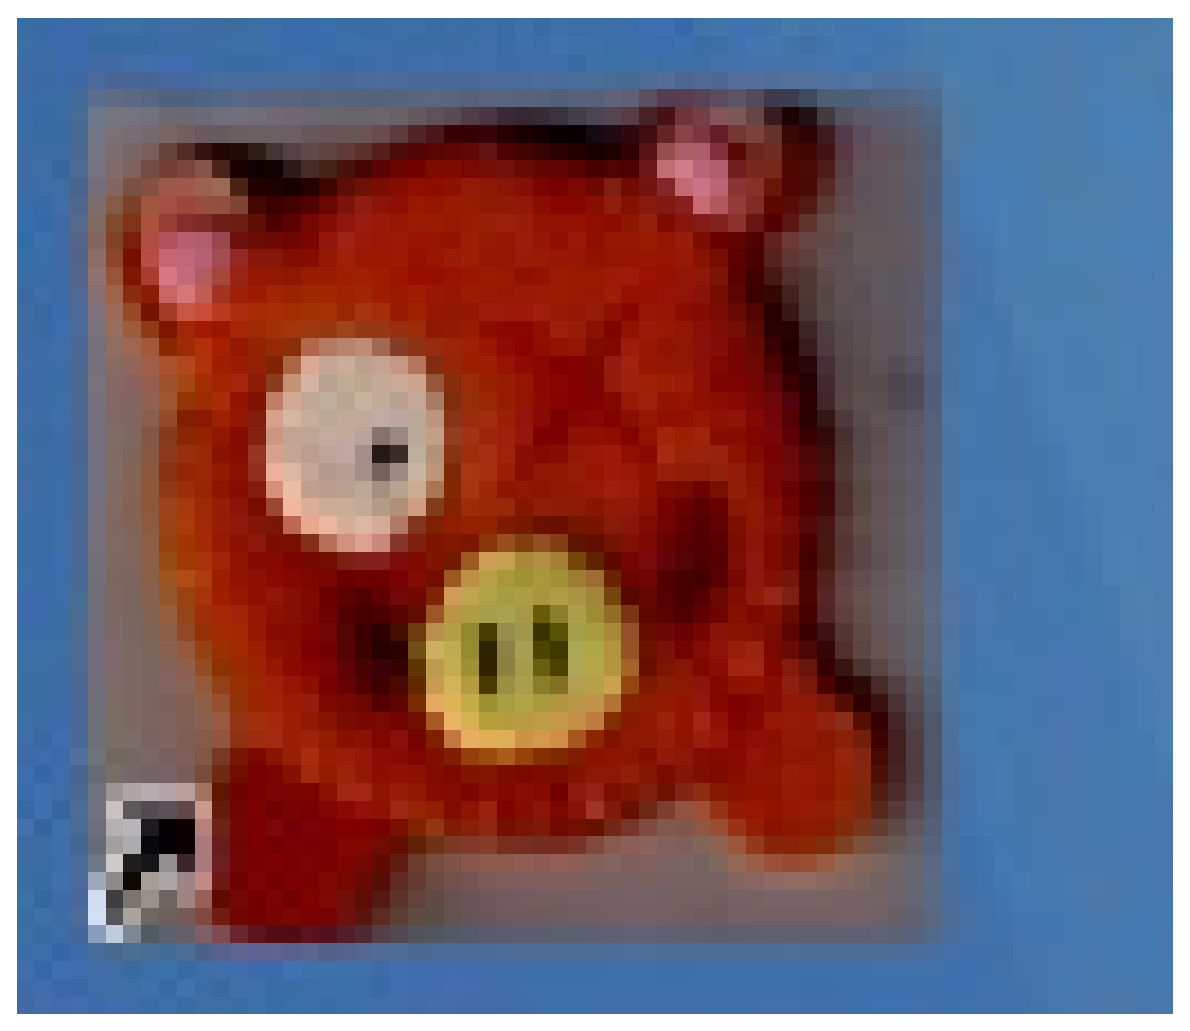
\includegraphics{Figs/inobuta.ps}}
\end{center}
%>C
$B$r%@%V%k%/%j%C%/$9$k$H?^(B\ref{fig:cfepStart}$B$N$h$&$K(B cfep/asir $B$,5/F0$9$k(B.
$B0J2<(B cfep/asir $B$rC1$K(B asir $B$H$h$V(B.

%<C
\begin{figure}[tb]
\scalebox{0.5}{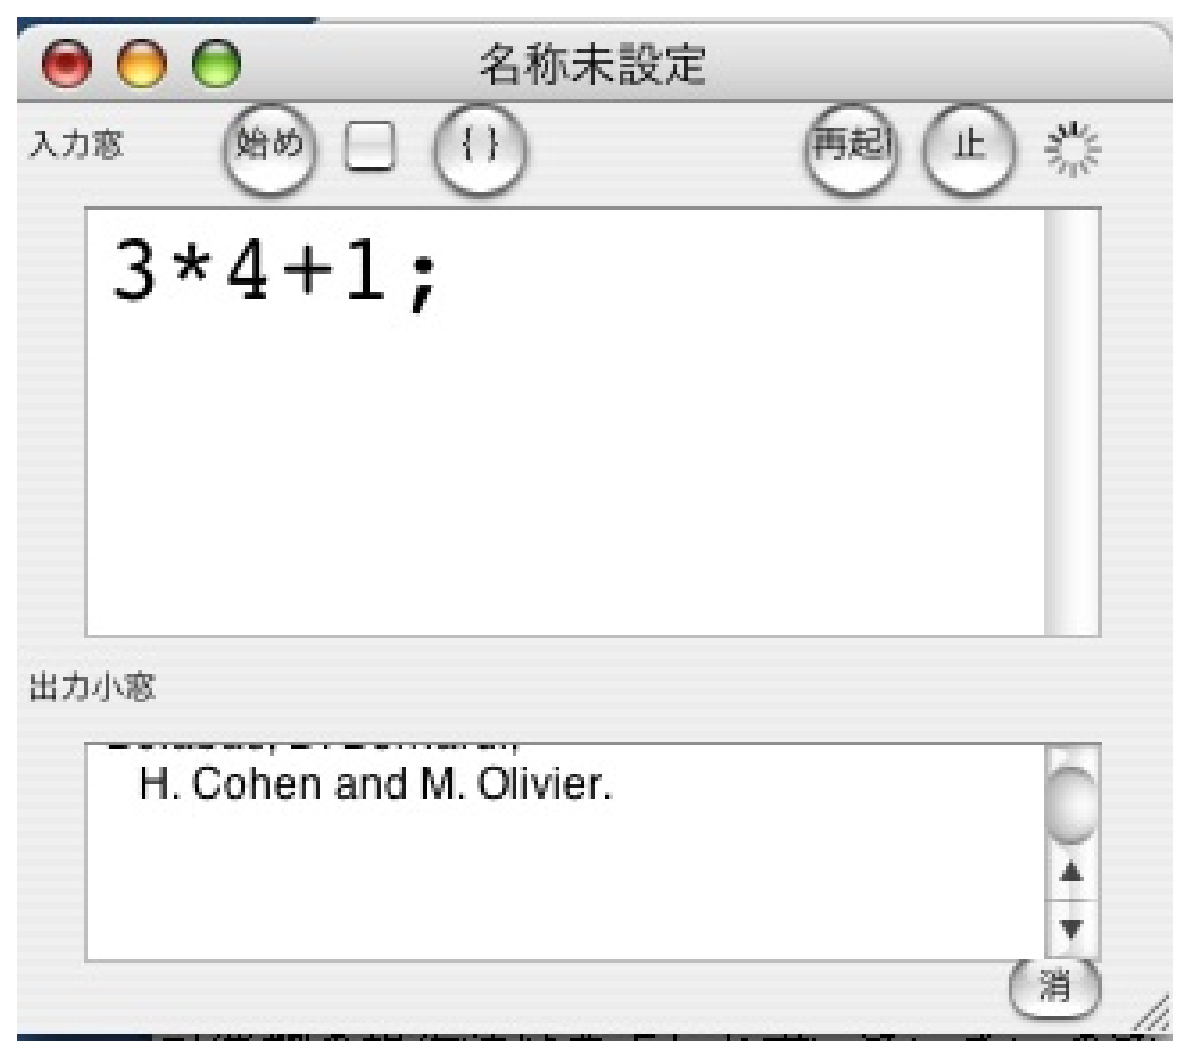
\includegraphics{Figs/cfepStart.ps}}
\caption{ cfep/asir $B$N5/F02hLL(B} \label{fig:cfepStart}
\end{figure}
%>C

$B?^(B\ref{fig:cfepStart} $B$NF~NOAk$K7W;;$7$?$$<0$d%W%m%0%i%`$rF~NO$7$F(B
``$B;O$a(B''$B%\%?%s(B
%<C
\begin{center}
\scalebox{0.1}{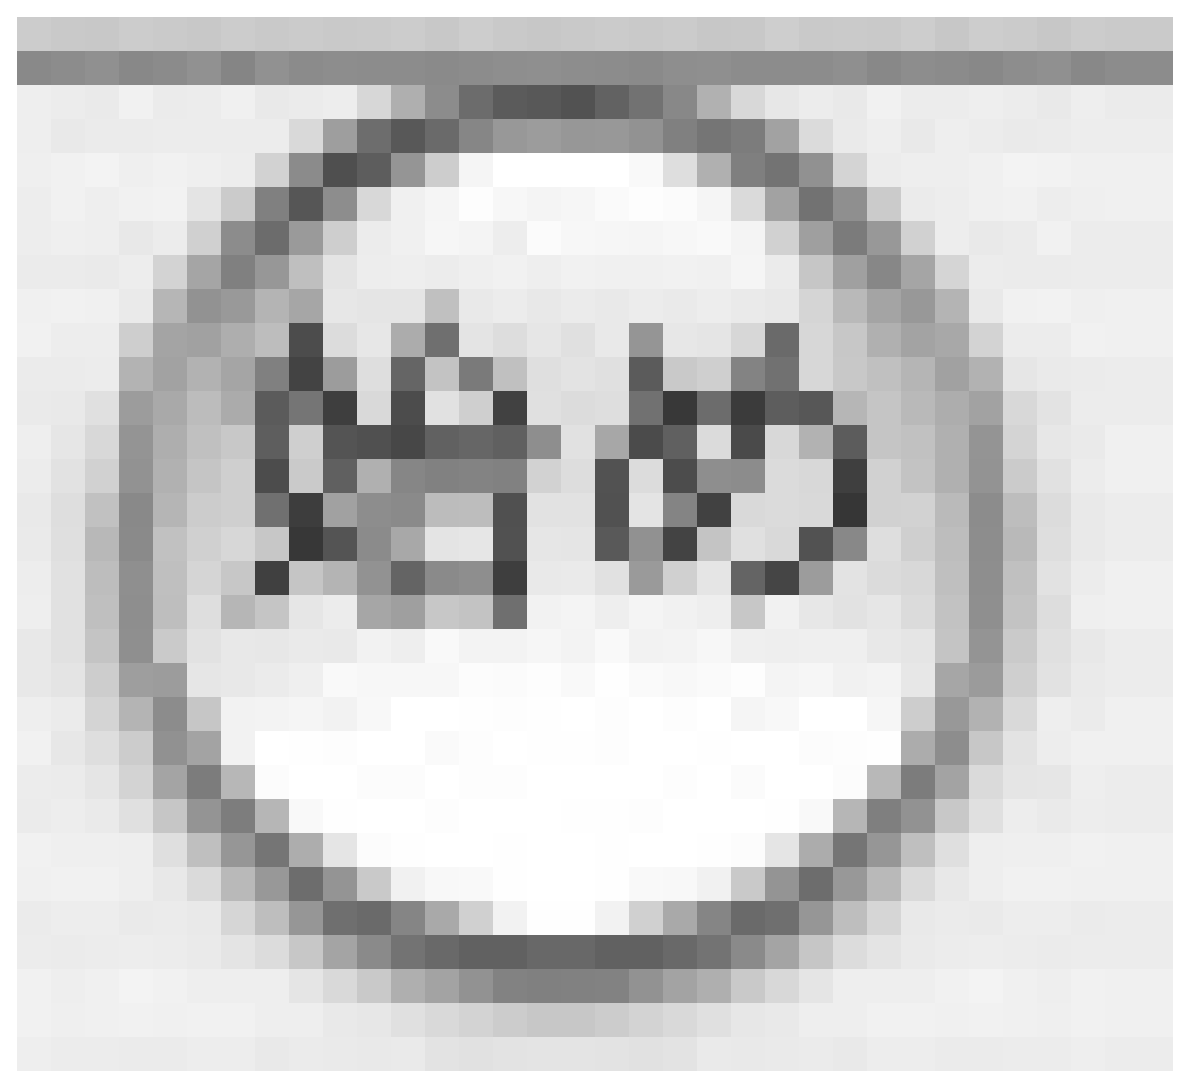
\includegraphics{Figs/buttonStart.ps}}
\end{center}
%>C
$B$r$*$9$H<B9T$r3+;O$9$k(B.
$B<0$N7W;;$d%W%m%0%i%`$N<B9T$,=*N;$9$k$H(B,
$B?7$7$$%&%$%s%I%&(B OutputView $B$,3+$-7k2L$,$=$N%&%$%s%I%&$KI=<($5$l$k(B.
\index{$B$K$e$&$j$g$/$^$I(B@$BF~NOAk(B}
\index{OutputView}
``$B;O$a(B''$B%\%?%s$r$*$7$F<B9T$r3+;O$9$k$3$H$r7W;;5!MQ8l$G$O(B 
``$BF~NO$NI>2A$r;O$a$k(B'' $B$H$$$&(B.
\index{;}  \index{$B$R$g$&$+(B@$BI>2A(B}

$B=PNO>.Ak$K$O%7%9%F%`$+$i$N$$$m$$$m$J>pJs$,=PNO$5$l$k$,(B,
$BFbMF$OCf>e5i<T8~$1$N$b$N$,B?$$(B.
\index{$B$7$e$D$j$g$/$3$^$I(B@$B=PNO>.Ak(B}

$B%U%!%$%k%a%K%e!<(B
%<C
\begin{center}
\scalebox{0.3}{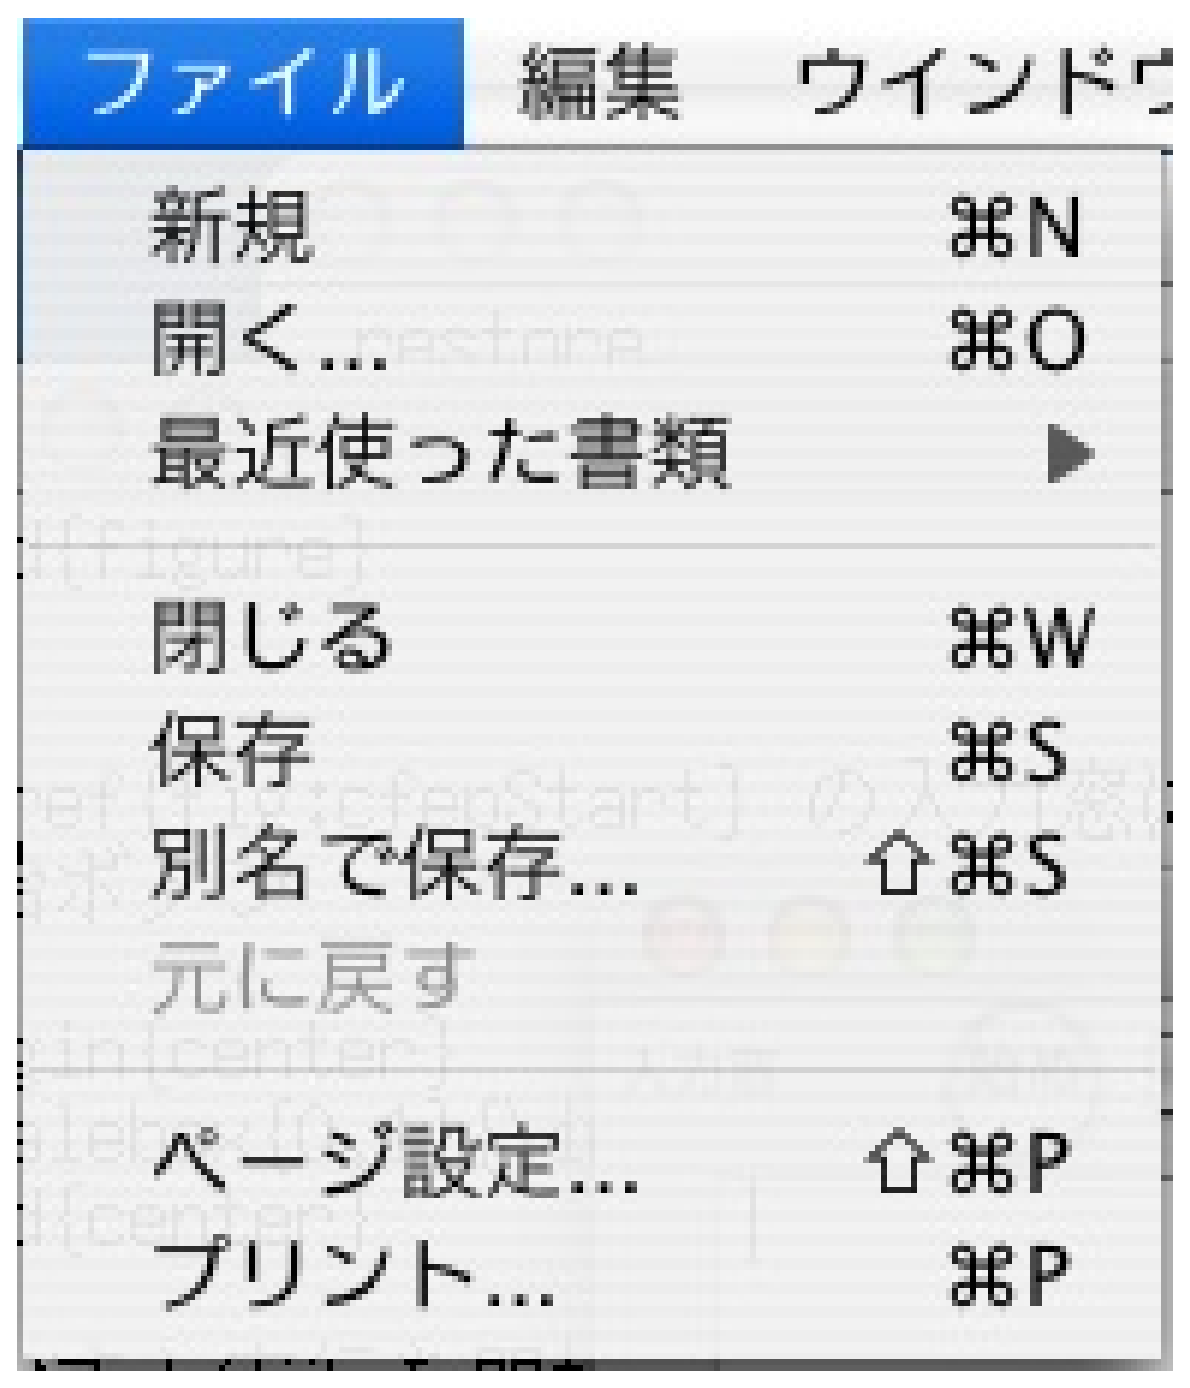
\includegraphics{Figs/menuFile.eps}}
\end{center}
%>C
$B$+$i(B''$BJ]B8(B''$B$d(B''$BJLL>$GJ]B8(B''$B$r<B9T$9$k$HF~NOAk$NFbMF$r%U%!%$%k$H$7$FJ]B8$G$-$k(B.
$B=PNO>.Ak$NFbMF$d(B OutputView $B$NFbMF$OJ]B8$5$l$J$$$N$GCm0U$7$F$[$7$$(B.

cfep/asir $B$r40A4$K=*N;$9$k$K$O(B cfep $B%a%K%e!<(B
%<C
\begin{center}
\scalebox{0.3}{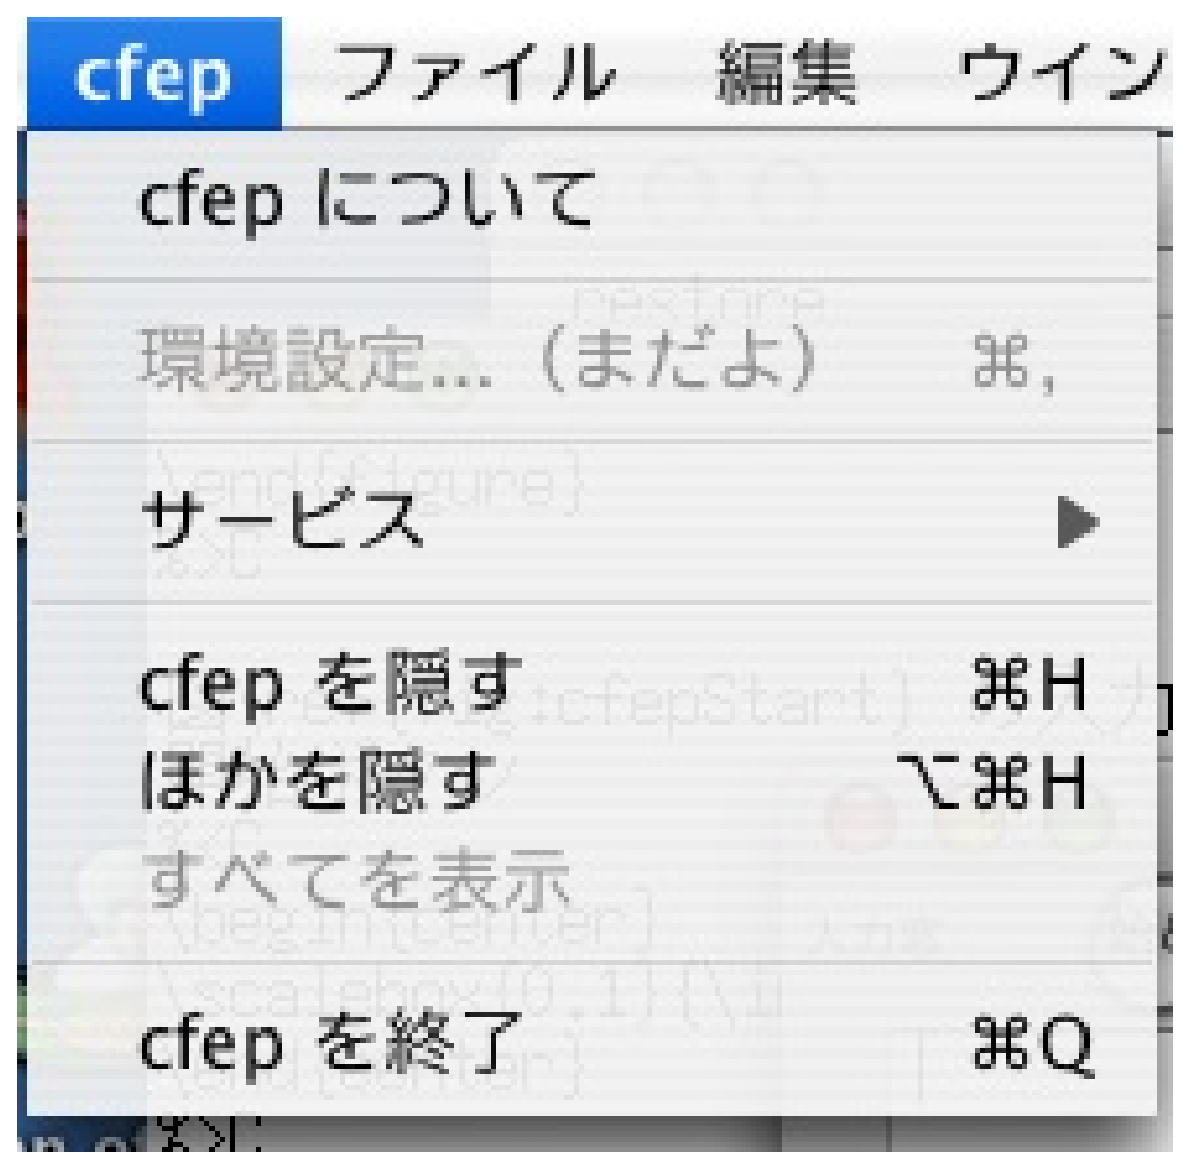
\includegraphics{Figs/menuCfep.eps}}
\end{center}
%>C
$B$N(B ``cfep $B$r=*N;(B'' $B$r<B9T$9$k(B.
%en Input \verb@ quit; @ to terminate the Risa/Asir.
%
%

%<C
\bigbreak
\bigbreak

%>C


$B$5$F?^(B\ref{fig:cfepStart}$B$G$O(B
$ 3 \times 4 + 1 $ $B$N7W;;$r$7$F$$$k(B.
\begin{screen}
Asir $B$K$*$1$k7W;;<0$OIaDL$N?t<0$H;w$F$$$F(B,
$BB-$7;;$O(B {\tt $+$},
$B0z$-;;$O(B {\tt $-$}
$B$H=q$/(B.
$B$+$1;;$H3d;;$O(B $\times$ $B$d(B $B!`(B $B$,%-!<%\!<%I$K$J$$$H$$$&Nr;KE*M}M3$b$"$j(B,
$B$=$l$>$l(B {\tt *} $B$H(B {\tt /} $B$GI=8=$9$k(B.
$BN_>h(B $P^N$ $B$O(B \verb@P^N@ $B$N$h$&$K(B \verb@^@ $B5-9f$rMQ$$$FI=$9(B.
\end{screen}

\begin{screen}
$B<0$N=*$j$r=hM}7O(B(asir)$B$K65$($k(B($B<($9(B)$B$N$K(B {\tt ;} ($B%;%_%3%m%s(B)
$B$r=q$+$J$$$H$$$1$J$$(B.
$BJ8Kv$N(B ``$B!#(B'' $B$N$h$&$JLr3d$r2L$?$9(B.
$B$^$?$+$1;;$N5-9f(B {\tt *} $B$N>JN,$O$G$-$J$$(B. 
\end{screen}

\begin{example} \rm
$B0J2<$N:8$N7W;;<0$r(B asir $B$G$O1&$N$h$&$K$"$i$o$9(B.
\begin{center}
\begin{tabular}{|l|l|} \hline
$2 \times (3+5^4)$  &    \verb@2*(3+5^4);@  \\ \hline
$\left\{\left(2+\frac{2}{3}\right)\times 4+\frac{1}{3}\right\}\times 2 +5  $
                         & \verb@ ((2+2/3)*4+1/3)*2+5; @ \\ \hline
$AX+B$  & \verb@A*X+B;@ \\ \hline
$AX^2+BX+C$ & \verb@A*X^2+B*X+C;@ \\ \hline
$\frac{1}{X-1}$ & \verb@1/(X-1);@ \\ \hline
\end{tabular}
\end{center}
\end{example}

$B7W;;$N=g=x$O3g8L$b4^$a$FIaDL$N?t<0$N7W;;$HF1$8$G$"$k(B. 
$B$?$@$7(B
$B?t3X$G$O$+$C$3$H$7$F(B, {\tt [,]},{\tt \{,\}}$B$J$I$,$D$+$($k$,(B
asir $B$G$O(B {\tt (,)} $B$N$_(B.
{\tt [,]} $B$d(B {\tt \{,\}}$B$OJL$N0UL#$r$b$D(B.
$B>e$NNc$N$h$&$K(B {\tt (,)} $B$r2?=E$K$b$D$+$C$F$h$$(B.
%en In mathematics, {\tt (,)}, {\tt [,]} ,{\tt \{,\}} are used 
%en as brackets in expressions,
%en but in Risa/Asir,  only {\tt (,)} can be used as brackets in expressions,
%en and {\tt [,]} and {\tt \{,\}} are used for different purposes (list and
%en grouping in programs).
$B$3$N>l9g3g8L$NBP1~4X78$,$o$+$j$K$/$$(B.
$B3g8L$NBP1~$rD4$Y$?$$HO0O$r%^%&%9$G%I%i%C%0$7$FA*Br$7(B,
\begin{center}
  \scalebox{0.1}{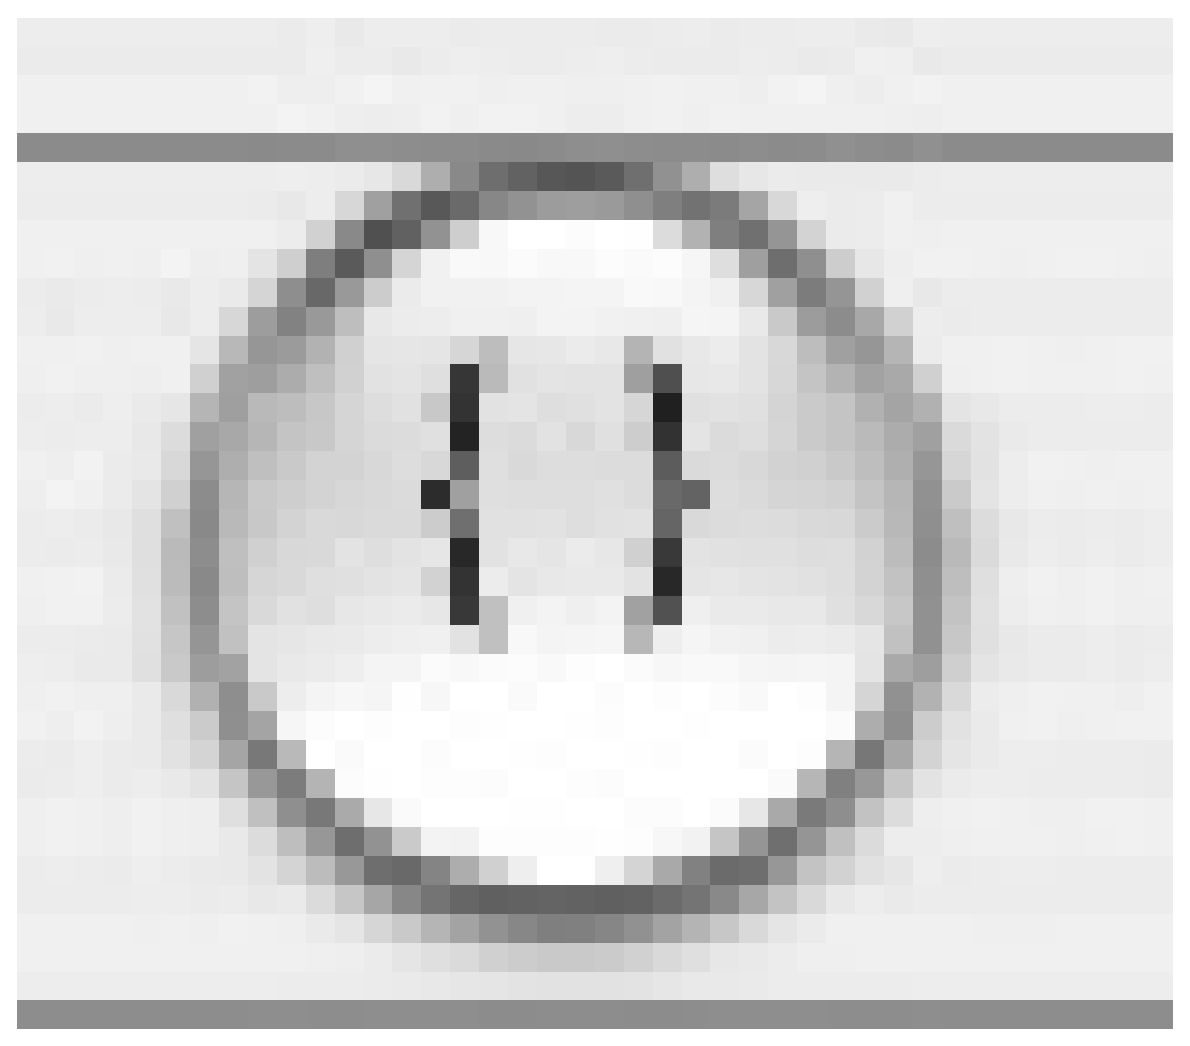
\includegraphics{Figs/buttonBracket.eps}}
\end{center}
$B%\%?%s$r$*$9$3$H$K$h$j3g8L$NBP1~$rD4$Y$k$3$H$,$G$-$k(B.
\begin{figure}[tb]
\begin{center}
  \scalebox{0.5}{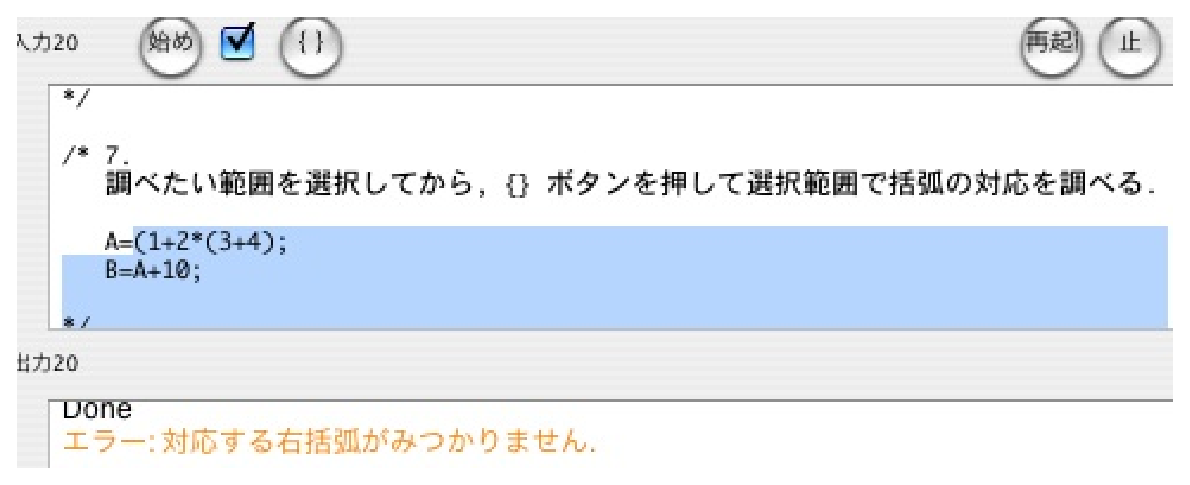
\includegraphics{Figs/menuCheckBracket.eps}}
\end{center}
\caption{$B3g8L$NBP1~(B} \label{fig:menuCheckBracket}
\end{figure}
$B?^(B\ref{fig:menuCheckBracket}$B$NNc$G$O(B \verb@(1+2*(3+4))@ $B$H=q$/$Y$-$H$3$m$r(B
\verb@(1+2*(3+4)@ $B$H=q$$$F$*$j%(%i!<$,I=<($5$l$F$$$k(B. 

\bigbreak

\noindent \QQQ
``Basic$BIw$N;H$$J}$r@bL@$9$k(B'' $B$H=q$$$F$"$j$^$7$?$,(B, Basic $B$C$F2?$G$9$+(B? \\
\noindent \AAA
$B%3%s%T%e!<%?$K;E;v$r$5$;$k$K$O:G=*E*$K$O%W%m%0%i%`8@8l(B
($B7W;;5!$X$N;E;v$N<j=g$r;X<($9$k$?$a$N?M9)8@8l(B)$B$rMQ$$$k(B.
$B%o!<%W%mEy$b%W%m%0%i%`8@8l$G5-=R$5$l$F$$$k(B.
Basic $B$O:G$b8E$$%W%m%0%i%`8@8l$N0l$D$G$"$j(B, $B=i?4<T$K$d$5$7$/(B, $B$+$D(B
$B7W;;5!$N;EAH$_$d%W%m%0%i%`8@8l$NM}2r$K$bM-MQ$G$"$k(B.
Basic $B$O9b9;$N?t3X$N652J=qEy$K$bEP>l$9$k(B.
$BCx<T$O$$$^$^$G(B ``10$B?J(BBASIC'' $B$r=i?4<T8~$165:`$H$7$F3hMQ$7$F$$$?$,(B, 
``10$B?J(BBASIC''$B$,(B MacOS X $B$GF0:n$7$J$$$?$a(B cfep $B$r3+H/$7$?(B.
Asir $B8@8l$b%W%m%0%i%`8@8l$G$"$j(B Basic $B$H$h$/;w$F$$$k$,(B, C $B8@8l$K$b$C$H6a$$(B.


\noindent \QQQ
MacOS X $B$C$F2?$G$9$+(B? \\
\noindent \AAA
-----$B$^$@=q$$$F$J$$(B.



%<C
\bigbreak
\noindent
%>C
Asir $B$O?t$N=hM}$N$_$J$i$:(B, $\sqrt{x}$$B$d;03Q4X?t$N6a;w7W;;(B, $BB?9`<0$N7W;;$b$G$-$k(B.
%en Asir can do calculations not only for numbers, but also for polynomials.
%en Let us see some examples.
%en 
$B:8$N?t3XE*$J<0$O(B asir $B$G$O1&$N$h$&$KI=$9(B.
\begin{center}
\begin{tabular}{|l|l|} \hline
 $\pi$ ($B1_<~N((B) &  {\tt @pi} \\ \hline
 $\cos x$ & {\tt cos(x)} \\ \hline
 $\sin x$ & {\tt sin(x)} \\ \hline
 $\tan x$ & {\tt tan(x)} \\ \hline
 $\sqrt{x}$ & \verb@x^(1/2)@ \\ \hline
\end{tabular}
\end{center}
%en {\tt sin(x), cos(x)} are the trigonometric functions sine and cosine.
%en The symbol {\tt @pi} is the constant $\pi$.
$B;03Q4X?t$N3QEY$K$"$?$kItJ,$N(B $x$ $B$O%i%8%"%s$H$$$&C10L$rMQ$$$FI=$9(B.
$B9b9;Dc3XG/$N?t3X$G$O3QEY$rEY(B(degree)$B$H$$$&C10L$rMQ$$$FI=$9$,(B,
$B?t3X(B3$B0J>e$G$O3QEY$O%i%8%"%s$H$$$&C10L$GI=$9(B.
\begin{screen}
90$BEY(B($BD>3Q(B)$B$,(B $\pi/2$ $B%i%8%"%s(B, 180$BEY$,(B $\pi$ $B%i%8%"%s(B.
$B0lHL$K(B $d$$BEY$O(B $\frac{d}{180} \pi$ $B%i%8%"%s$G$"$k(B.
\end{screen}
$BC10L%i%8%"%s$r$b$A$$$k$HHyJ,K!$N8x<0$,4J7i$K$J$k(B.
$B$?$H$($P(B $x$ $B$,%i%8%"%s$G$"$k$H(B $\sin x$ $B$NHyJ,$O(B $\cos x$ $B$G$"$k(B.
\index{$B$i$8$"$s(B@$B%i%8%"%s(B}

$\sin(x)$ $B$d(B $\cos(x)$ $B$N6a;wCM$r5a$a$k$K$O$?$H$($P(B
%en \item  In order to get approximate values of $\sin(x)$  $\cos(x)$, input as
%<C
\begin{center}
\verb@  deval(sin(3.14));  @ 
\end{center}
%>C
$B$HF~NO$9$k(B.   
$B$3$l$O(B $\sin (3.14)$ $B$N6a;wCM$r7W;;$9$k(B.
$\sin \pi = 0 $ $B$J$N$G(B $0$ $B$K6a$$CM$,=PNO$5$l$k$O$:$G$"$k(B.
$B<B:](B {\tt 0.00159265} $B$r=PNO$9$k(B.  \index{deval}
{\tt deval}  
(\underline{eval}uate and get a result in {\underline d}ouble number precision $B$NN,(B)
$B$O(B 64 bit$B$NIbF0>.?tE@?t$K$h$j6a;wCM7W;;$9$k(B. 
64 bit$B$NIbF0>.?tE@?t$H$O2?$+$N@bL@$OD6F~Lg$NHO0O30$G$"$k$,(B,
$B7W;;5!$OM-8B$N5-21NN0h(B($B%a%b%j(B)$B$7$+;}$?$J$$$N$G(B, $B>.?t$bM-8B7e$7$+07$($J$$(B
$B$H3P$($F$*$3$&(B. 64bit $B$O07$($k7e?t$rI=$7$F$$$k(B.
$B>\$7$/$O(B ``asir $B%I%j%k(B'' $B$r;2>H$7$FM_$7$$(B.

%en The function {\tt deval} numerically evaluates the argument in 64 bit floating point arithmetic.
%en As to details, see Chapter \ref{chapter:naibu}.
%en 

\begin{figure}[thb]
\begin{center}
  \scalebox{0.5}{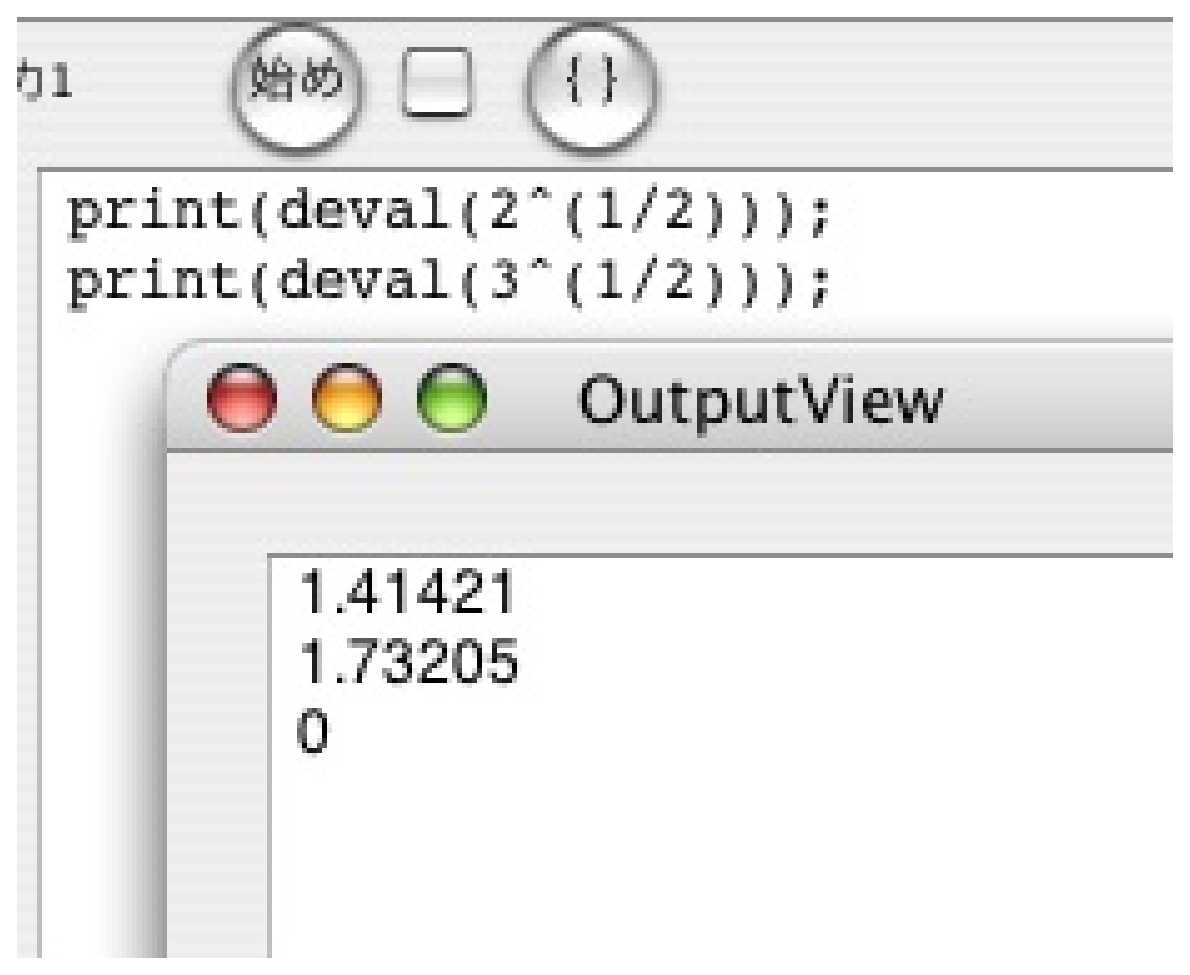
\includegraphics{Figs/sqrt2.eps}} 
\end{center}
\caption{$BJ?J}:,$N7W;;(B}
\label{fig:sqrt2}
\end{figure}

\begin{example} \rm
$\sqrt{2}$, $\sqrt{3}$ $B$N6a;wCM$r7W;;$7$J$5$$(B. \\
$BF~NO(B
\begin{screen}
\begin{verbatim}
  print(deval(2^(1/2)));
  print(deval(3^(1/2)));
\end{verbatim}
\end{screen}
$B=PNO$O(B
$B?^(B\ref{fig:sqrt2}$B$r$_$h(B.
\end{example}


$B>e$NNc$N$h$&$K(B,
$B%;%_%3%m%s(B {\tt ;} $B$G6h@Z$i$l$?0lO"$NL?Na$N$"$D$^$j$O$b$C$H$b(B
$BC1=c$J(B asir $B%W%m%0%i%`$NNc$G$"$k(B.  \index{$B$W$m$0$i$`(B@$B%W%m%0%i%`(B}
$B0lO"$NL?Na$O;O$a$+$i=gHV$K<B9T$5$l$k(B.
{\tt print($B<0Ey(B);} $B$O(B ``$B<0Ey(B'' $B$NCM$r7W;;$7$FCM$r2hLL$KI=<($9$k(B.

$B$5$F=PNO$N(B {\tt 1.41421} ($B$R$H$h(B $B$R$H$h$K(B $B$R$H$_$4$m(B) $B$O(B $\sqrt{2}$ $B$N6a;wCM$J$N$G(B,
\verb@print(deval(2^(1/2)));@
$B$N<B9T7k2L$G$"$k(B. 
$B$5$F=PNO$N(B {\tt 1.73205} ($B$R$H$J$_$K(B $B$*$4$l$d(B) $B$O(B $\sqrt{3}$ $B$N6a;wCM$J$N$G(B,
\verb@print(deval(3^(1/2)));@
$B$N<B9T7k2L$G$"$k(B. 
$B:G8e$N(B {\tt 0} $B$O$J$s$J$N$G$"$m$&$+(B?
$B<B$O$3$l$O:G8e$N(B {\tt print} $BJ8$NLa$7$F$$$kCM$G$"$k(B.
$B$`$D$+$7$$(B? $BJL$NNc$G@bL@$7$h$&(B.

\noindent
\fbox{$BF~NO(B}
\begin{screen}
\begin{verbatim}
1+2;
2+3;
3+4;
\end{verbatim}
\end{screen}
$B$3$N;~=PNO$O(B(OutputView$B$X$NI=<($O(B)
\begin{screen}
{\tt 7}
\end{screen}
$B$H$J$k(B.
cfep/asir $B$G$O$H$/$K(B {\tt print} $BJ8$r$+$+$J$$8B$j(B
$B:G8e$NJ8$N7W;;7k2L(B($BI>2A7k2L(B)$B$7$+=PNO$7$J$$(B.
$B$$$^$N>l9g$O(B $3+4$  $B$N7k2L(B $7$ $B$r=PNO$7$F$$$k(B.
\index{$B$7$e$D$j$g$/$1$C$+(B@$B=PNO7k2L(B}

\begin{problem} \rm
\begin{enumerate}  \index{2$B$N$k$$$8$g$&(B@$2$$B$NN_>h(B}
\item $2^8$, $2^9$, $2^{10}$, 
$B$NCM$r7W;;$7$FEz$($rI=<($9$k%W%m%0%i%`$r=q$-$J$5$$(B.
\item $2$ $B$NN_>h$O%Q%=%3%s$N@-G=@bL@$K$h$/EP>l$9$k(B.
$B$?$H$($P8!:w%7%9%F%`(B google $B$K%-!<%o!<%I(B ``512 $B%a%b%j(B $BEk:\(B'' $B$rF~NO$7$?$H$3$m(B
``$B%S%G%*%a%b%j$r(B 256M $B$+$i(B 512M $B$KG\A}$5$;(B'' $B$J$I(B, $B?tB?$/$N5-;v$,%R%C%H$9$k(B.
$B$3$N$h$&$J5-;v$r(B($B0UL#$,$o$+$i$J$/$F$b(B)10$B7o$"$D$a$F$_$h$&(B.
$512$ $B0J30$N(B $2$ $B$NN_>h$G$bF1$8$3$H$r;n$7$F$_$h$&(B.
\item ($BCf5i(B) $2$ $B$NN_>h$,%Q%=%3%s$N@-G=@bL@$K$h$/EP>l$9$kM}M3$rO@$8$J$5$$(B.
\end{enumerate}
\end{problem}

\bigbreak

\begin{figure}[thb]
\begin{center}
  \scalebox{0.4}{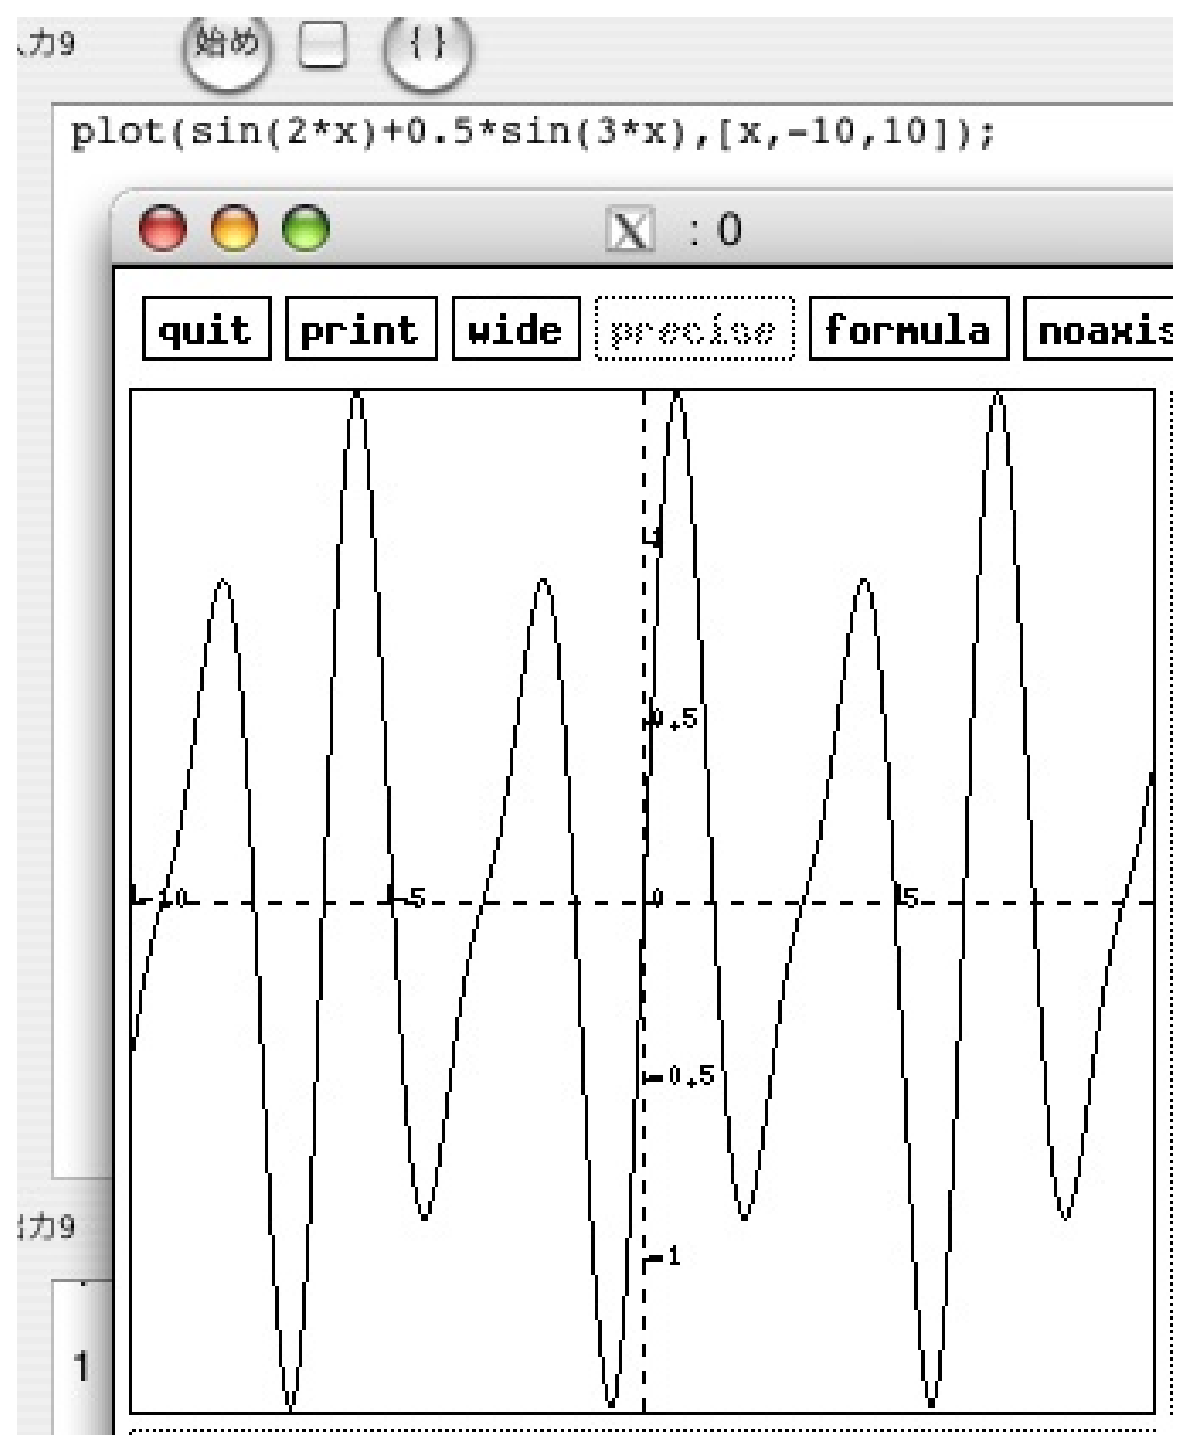
\includegraphics{Figs/plot1.eps}} 
\end{center}
\caption{$B4X?t$N%0%i%U(B}
\end{figure}

\noindent
\HHH
\index{plot}  \index{X11}
%en \begin{example} \rm
%en \index{plot}
\underline{X11 $B4D6-$,F0$$$F$$$l$P(B},
{\tt plot(f);}   $BL?Na$G(B
$x$$B$N4X?t(B $f$ $B$N%0%i%U$rIA$1$k(B.
%en The command {\tt plot(f);}   
%en draws the graph of the function $f$ in the variable $x$.
{\tt x} $B$NHO0O$r;XDj$7$?$$$H$-$O$?$H$($P(B  \\
{\tt plot(f,[x,0,10])}
$B$HF~NO$9$k$H(B, {\tt x} $B$O(B 0 $B$+$i(B 10 $B$^$GJQ2=$9$k(B.
%en When you need to specify the range of variables {\tt x}, 
%en input, for example  \\
%en {\tt plot(f,[x,0,10])}
%en Then, the variable {\tt x} runs over $[0, 10]$.

\noindent \fbox{$BF~NONc(B}
%<C
\begin{screen}
\begin{verbatim}
    plot(sin(x));  
    plot(sin(2*x)+0.5*sin(3*x),[x,-10,10]);  
\end{verbatim}
\end{screen}
%>C
\begin{problem} \rm
$B$$$m$$$m$J4X?t$N%0%i%U$rIA$$$F$"$=$s$G$_$h$&(B.
$B?t3X$NCN<1$rAmF00w$7$F7W;;5!$NIA$/7A$,$I$&$7$F$=$&$J$N$+(B
$B@bL@$r;n$_$F$_$h$&(B.
\end{problem}


\section{$B%(%i!<%a%C%;!<%8(B}

$BF~NO$K%(%i!<$,$"$k$H(B, $B%(%i!<%a%C%;!<%8$,I=<($5$l$k(B.
\index{$B$($i!<(B@$B%(%i!<(B}
\index{$B$($i!<$a$C$;!<$8(B@$B%(%i!<%a%C%;!<%8(B}

\begin{figure}[htb]
\begin{center}
  \scalebox{0.5}{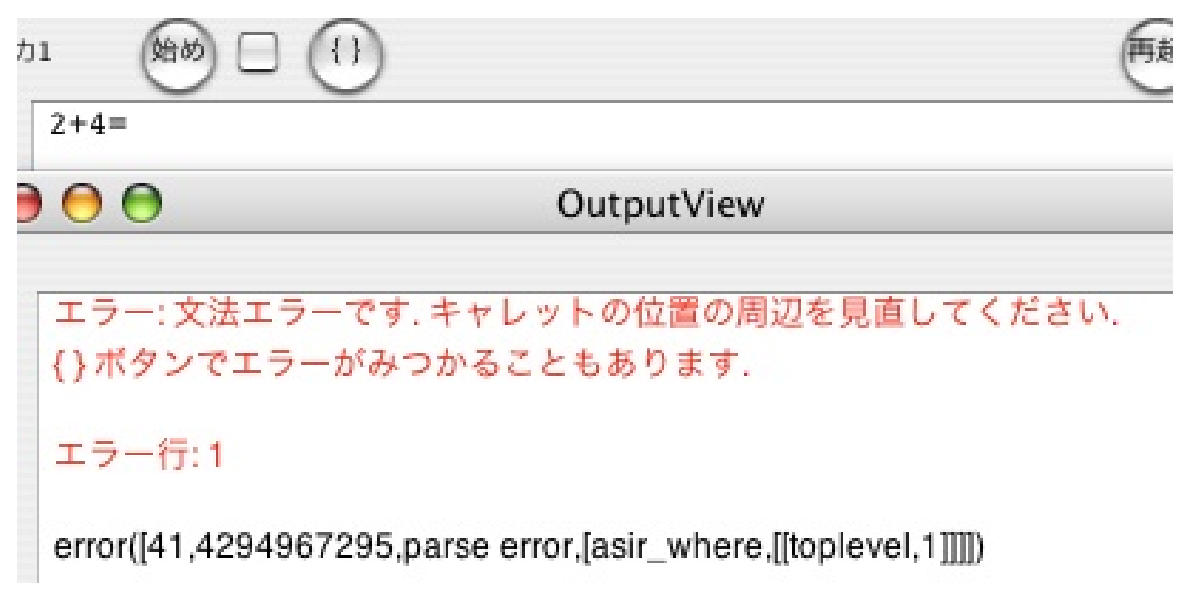
\includegraphics{Figs/errorParseEq}}
\end{center}
\caption{$BJ8K!%(%i!<(B} \label{fig:errorParseEq}
\end{figure}
$B?^(B\ref{fig:errorParseEq} $B$G$O(B
\verb@ 2+4= @
$B$HF~NO$7$F$$$k(B. $B:G8e$K(B \verb@=@ $B$r=q$/I=8=$O(B asir $B$NJ8K!$G$O(B
$B5v$5$l$F$$$J$$$N$G(B,  ``$BJ8K!%(%i!<(B'' $B$H;XE&$5$l$F$$$k(B.  \index{$B$V$s$]$&$($i!<(B@$BJ8K!%(%i!<(B}
\begin{screen}
$BBgBN$3$l$G$o$+$C$F$/$l$F$$$$$8$c$J$$(B,
$B$H$3$A$i$,$*$b$C$F$$$F$b%W%m%0%i%`8@8l$O0l@ZM;DL$,$-$+$J$$(B.
\end{screen}
$B$J$*(B
\begin{verbatim}
error([41,4294967295,parse error,[asir_where,[[toplevel,1]]]])
\end{verbatim}
$B$NItJ,$O>e5i<T8~$1$N>pJs$J$N$G$H$j$"$($:L5;k$7$F$b$i$$$?$$(B.


\begin{figure}[htb]
\begin{center}
  \scalebox{0.5}{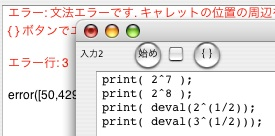
\includegraphics{Figs/errorMultiLine}}
\end{center}
\caption{$B%(%i!<9T(B} \label{fig:errorMultiLine}
\end{figure}
$B?^(B\ref{fig:errorMultiLine} $B$G$O(B
\begin{screen}
\begin{verbatim}
  print( 2^7 );
  print( 2^8 );
  print( deval(2^(1/2));
  print( deval(3^(1/2)));
\end{verbatim}
\end{screen}
$B$HF~NO$7$F$$$k(B. 
3$B9TL\$O1&3g8L$,$R$H$DB-$j$J$/$F(B
\verb@print( deval(2^(1/2)));@
$B$,@5$7$$F~NO$G$"$k(B.
$B%(%i!<9T$N(B3$B9TL\$K%-%c%l%C%H$,<+F0E*$K0\F0$7$F$$$k$O$:$G$"$k(B.
$B$J$*%W%m%0%i%`$NF~NO%&%$%s%I!<Fb$G%^%&%9$r%/%j%C%/$9$k$H(B, $B$;$C$+$/<+F00\F0$7$?(B
$B%-%c%l%C%H$N0LCV$,JQ$C$F$7$^$&(B. 
$B%W%m%0%i%`$NF~NO%&%$%s%I!<$N%?%$%H%k%P!<$G%/%j%C%/$9$k$H$h$$(B.
$B$J$*$3$NNc$G$O(B 
\begin{center}
\scalebox{0.05}{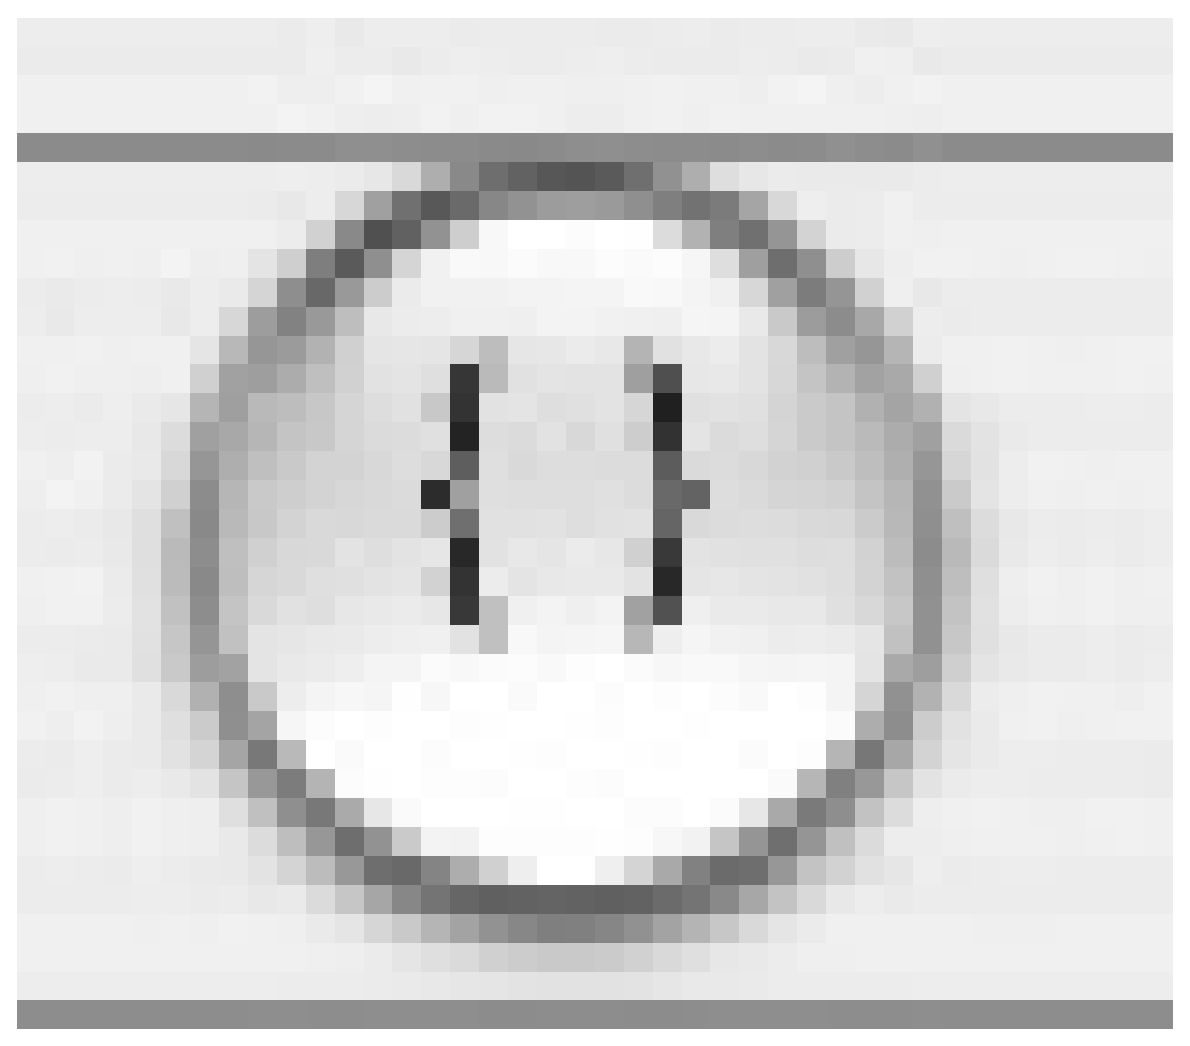
\includegraphics{Figs/buttonBracket.eps}}
\end{center}
$B%\%?%s$r$b$A$$$F$b$9$0%(%i!<$N>l=j$,$o$+$k(B.
\index{$B$+$C$3(B@$B3g8L(B}

\noindent {\bf $BCm0U(B}:
$BI=<($5$l$?9T$O%(%i!<$NH/@80LCV$G$"$k$,(B,
$B%(%i!<$N860x$O$=$NA0$NJ}$N9T$K$"$k$3$H$bB?$$(B.
$B$?$H$($P(B
\begin{screen}
\begin{verbatim}
1+2
2+3;
\end{verbatim}
\end{screen}
$B$HF~NO$9$k$H%(%i!<9T$O(B 2 $B9TL\$G$"$k$,(B, $B860x$O(B1$B9TL\$G(B {\tt ; } $B$r(B 
$B=q$-K:$l$?$3$H$G$"$k(B.

\bigbreak
$B%(%i!<9T$,J#?tI=<($5$l$?>l9g$O$=$l$i$NCf$N$I$3$+$K%(%i!<$,$"$k(B.
$BJ#?t$"$k%(%i!<9T$K=gHV$K%8%c%s%W$7$F$$$/$K$O(B,
\fbox{$B<B9T(B} $B%a%K%e!<$+$i(B \fbox{$B<!$N%(%i!<9T$X(B} $B$rA*Br$9$k(B.
\begin{center}
  \scalebox{0.3}{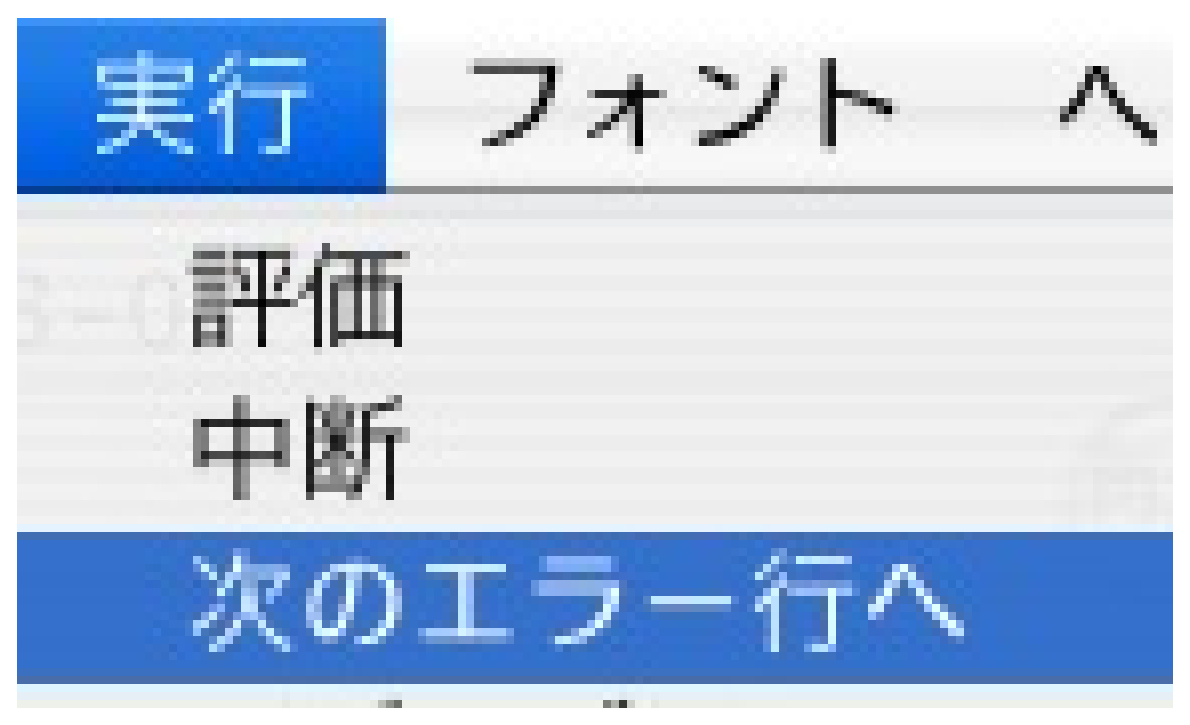
\includegraphics{Figs/menuNextError.eps}}
\end{center}
\index{$B$D$.$N$($i!<$.$g$&$X(B@$B<!$N%(%i!<9T$X(B}

\begin{problem} \rm
$B%(%i!<$r@8$8$k<0$^$?$O%W%m%0%i%`$r(B5$B$D:n$l(B.
\end{problem}


\chapter{ $BJQ?t$H%W%m%0%i%`(B }

\section{$BJQ?t(B}

\noindent  \index{$B$X$s$9$&(B@$BJQ?t(B}
$BJQ?t$K?tCMEy$r5-21$7$F$*$1$k(B.
\underline{$BJQ?tL>$OBgJ8;z$G;O$^$k(B}.  \index{$B$X$s$9$&$a$$(B@$BJQ?tL>(B}
%$B1Q;z$NBgJ8;z(B, $B;RJ8;z$r6hJL$7$F$$$k$N$GCm0U(B.
$B$J$*8e=R$9$k$h$&$K(B asir $B$G$OB?9`<07W;;$,$G$-$k$,>.J8;z$G;O$^$kJ8;zNs$O(B
$BB?9`<0$NJQ?tL>$H$7$FMxMQ$5$l$k(B.   
\index{$B$?$3$&$7$-$N$X$s$9$&$a$$(B@$BB?9`<0$NJQ?tL>(B}
%en \noindent
%en Symbols starting with capital alphabetical characters are 
%en {\it program variables}, which are used to store values.
%en \index{program variable}
%en Names of functions defined in programs start with small alphabetical 
%en characters.
%en Note that variable symbols starting with small alphabetical characters are
%en variables in polynomials in Risa/Asir and they cannot be used to store
%en values.
%en 

\index{2$B$N$k$$$8$g$&(B@$2$$B$NN_>h(B}
$2$$B$NN_>h$rI=<($9$k<!$N%W%m%0%i%`$r9M$($h$&(B.
\begin{screen}
\begin{verbatim}
 print( 2^1 );
 print( 2^2 );
 print( 2^3 );
 print( 2^4 );
 print( 2^5 );
 print( 2^6 );
 print( 2^7 );
 print( 2^8 );
\end{verbatim}
\end{screen}
$B$3$N%W%m%0%i%`$OJQ?t(B {\tt X} $B$rMQ$$$F(B
$B<!$N$h$&$K=q$$$F$*$1$P(B $2$ $B$NN_>h$@$1$J$/(B $3$ $B$NN_>h$rI=<($9$k(B
$B$N$K:FMxMQ$G$-$k(B($B?^(B\ref{fig:powerOf2}).
\begin{screen}
\begin{verbatim}
  X = 2;
  print( X^1 );
  print( X^2 );
  print( X^3 );
  print( X^4 );
  print( X^5 );
  print( X^6 );
  print( X^7 );
  print( X^8 );
\end{verbatim}
\end{screen}
\begin{figure}[thb]
\begin{center}
\scalebox{0.3}{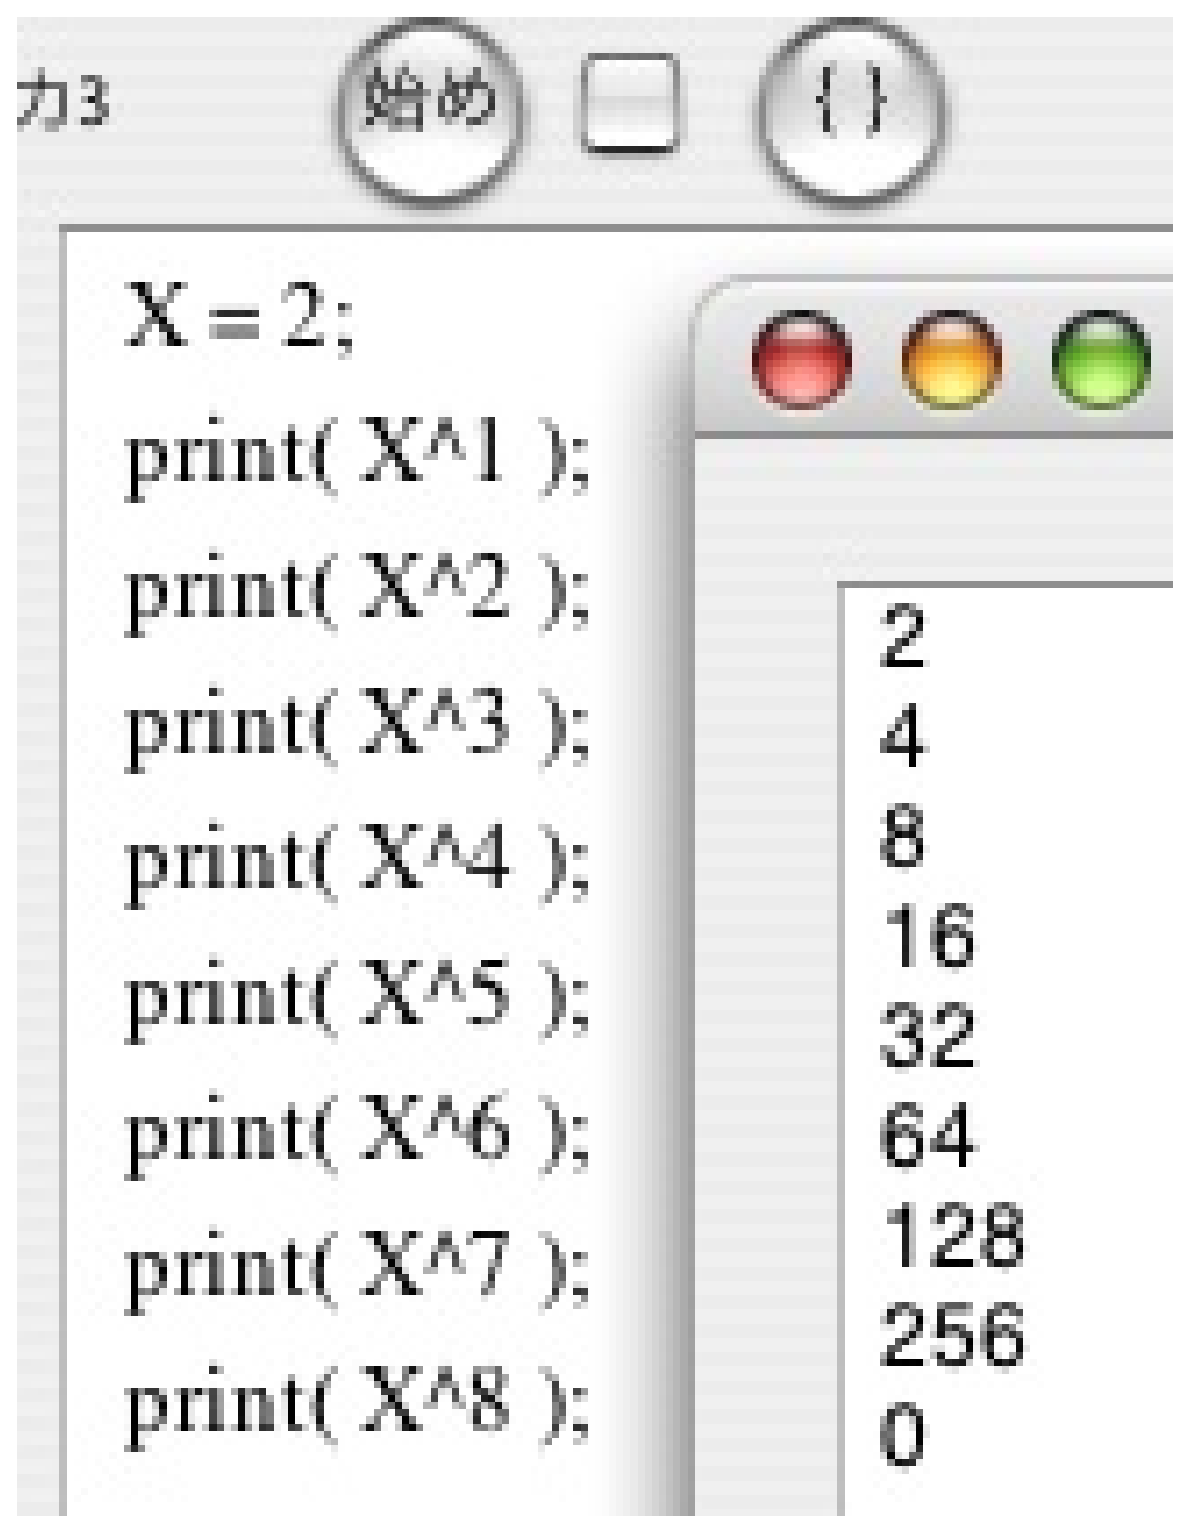
\includegraphics{Figs/powerOf2.eps}}
\end{center}
\caption{$BJQ?t$NMxMQ(B} \label{fig:powerOf2}
\end{figure}
$3$ $B$NN_>h$rI=<($9$k$K$O(B
\verb@X=2@ $B$N9T$r(B \verb@X=3@ $B$KJQ99$9$l$P$$$$$@$1$G$"$k(B.

$B%"%k%U%!%Y%C%H$N(B\underline{$BBgJ8;z(B}$B$G$O$8$^$k1Q?t;z$NNs$,(B asir $B$N(B
$BJQ?t$G$"$k(B.
$B$D$^$j(B, {\tt X}, {\tt Y}, {\tt Z} $B$O$b$A$m$s$N$3$H(B,
{\tt Sum} $B$H$+(B {\tt Kazu} $B$H$+(B {\tt X1} $B$J$I(B2$BJ8;z0J>e$N1Q?t;z$NNs(B
$B$NAH$_9g$o$;$,JQ?tL>$H$7$F5v$5$l$k(B.


$BJQ?t$r4^$s$@<0$r%W%m%0%i%`Cf$G<+M3$K$D$+$&$3$H$b$G$-$k(B.
$B$?$H$($P(B
\begin{verbatim}
  X = 2;
  A = 1;
  print( 2*X^2 -A );
\end{verbatim}
$B$r<B9T$9$k$H(B {\tt 7} $B$,I=<($5$l$k(B.

$B$3$N$h$&$JNc$r$_$k$H(B, $BJQ?t$N5!G=$O(B
$BCf3X?t3X$G$J$i$&J8;z<0$H;w$F$$$k$H;W$&$@$m$&(B.
$BD6F~Lg$H$7$F$O$3$l$G$[$\@5$7$$M}2r$G$"$k$,(B, $B$h$j%9%F%C%W%"%C%W$7$F$$$/$K$O(B,
$B<!$N$3$H$r6/$/5-21$7$F$*$3$&(B.
\begin{screen}
$BJQ?t$H$O7W;;5!$K?tCMEy$rJ]B8$7$F$*$/%a%b%j>e$N>l=j$NL>A0$G$"$k(B.
\end{screen}

$B$5$F(B, $BD6F~Lg(B, $BBh0l$N4XLg$G$"$k(B.
\begin{screen}
{\tt =} $B5-9f$O<!$N$h$&$J7A<0$G$D$+$&(B:
$$  \mbox{{\bf $BJQ?tL>(B}} {\tt = }  \mbox{{\bf $B<0(B}} {\tt  ;} $$
$B$3$l$O$^$:1&JU$N<0$r7W;;$7$=$N$"$H$=$N7W;;7k2L$r:8JU$NJQ?t$KBeF~$;$h$H$$$&0UL#(B. 
\verb@=@ $B5-9f$O1&JU$r7W;;$7$F$=$N7k2L$r:8JU$XBeF~$;$h$H$$$&(B\underline{$BL?Na(B}
$B$@$H;W$C$FM_$7$$(B. \\
$B$?$H$($P(B,
\verb@X=1@ $B$O(B \verb@X@ $B$,(B \verb@1@ $B$KEy$7$$$H$$$&0UL#$G$O$J$/(B,
\verb@1@ $B$r(B $BJQ?t(B \verb@X@ $B$KBeF~$;$h$H$$$&0UL#$G$"$k(B.
\end{screen}
$B$3$3$G$$$$$?$$$3$H$O(B,  \index{$B$@$$$K$e$&(B@$BBeF~(B} \index{=} \index{$B$@$$$K$e$&$-$4$&(B=@$BBeF~5-9f(B=}
\begin{screen}
\verb@=@ $B5-9f$N0UL#$,?t3X$G$N0UL#$H0c$&$h(B!
\end{screen}
$B$H$$$&$3$H$G$"$k(B.
$B$3$l$G:.Mp$9$kF~Lg<T$bB?$$$N$G%W%m%0%i%`8@8l$K$h$C$F$O(B
``$2$ $B$rJQ?t(B {\tt X} $B$KBeF~$;$h(B'' $B$r(B
\verb@X:=2@ 
$B$H=q$/>l9g$b$"$k(B ($B$?$H$($P%W%m%0%i%`8@8l(B Pascal).

$B<!$N%W%m%0%i%`$O(B $2$, $2^2$, $2^4$, $2^8$ $B$r7W;;$7$FI=<($9$k(B.
\begin{screen}
\begin{verbatim}
  X=2;
  print(X);
  X = X*X;
  print(X);
  X = X*X;
  print(X);
  X = X*X;
  print(X);
\end{verbatim}
\end{screen}
\begin{figure}[thb]
\begin{center}
\scalebox{0.3}{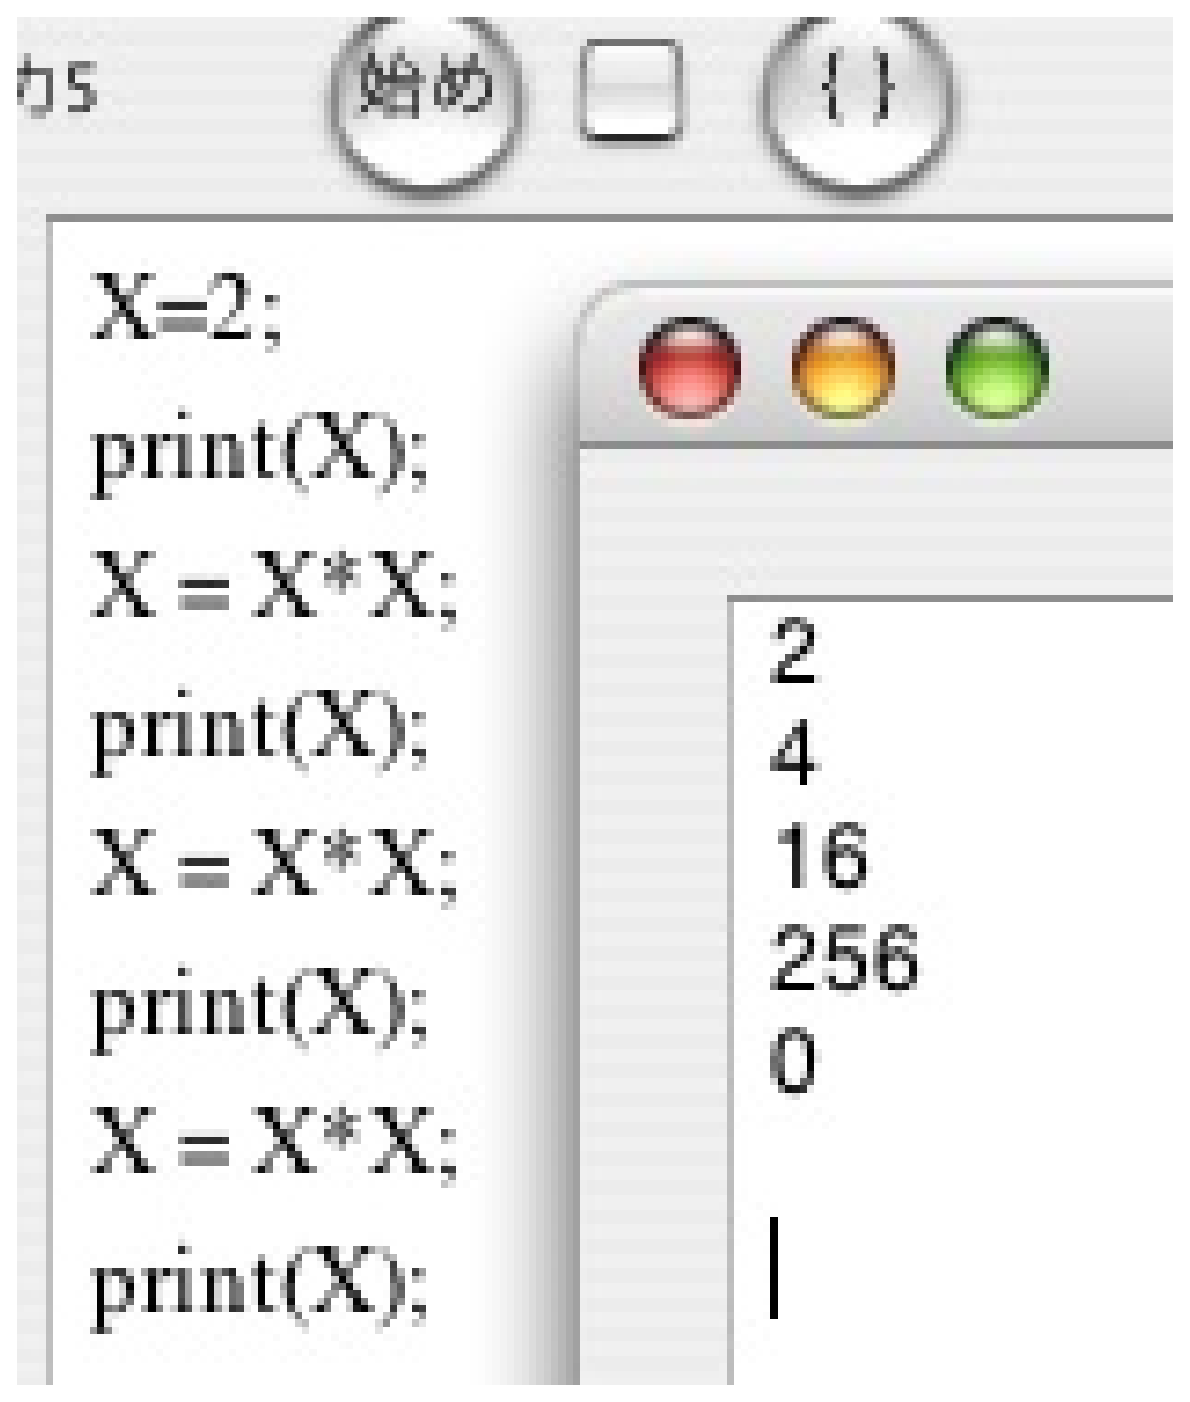
\includegraphics{Figs/powerOf2b.eps}}
\end{center}
\caption{$BJQ?t$NMxMQ(B} \label{fig:powerOf2b}
\end{figure}
$B=PNO$,?^(B\ref{fig:powerOf2b}$B$N$h$&$K$J$kM}M3$r@bL@$7$h$&(B.
$B$^$:(B1$B9TL\$GJQ?t(B{\tt X}$B$K(B2$B$,BeF~$5$l$k(B.
$B<!$K(B3$B9TL\$G$O$^$:1&JU$N<0$r7W;;$9$k(B. $B$3$N>l9g(B {\tt X} $B$NCM$O(B $2$ $B$G$"$k$N$G(B,
$2\times2$ $B$G7k2L$O(B $4$ $B$G$"$k(B.
\underline{$B$3$N7W;;$,=*$C$?8e(B}$B7k2L$N(B $4$ $B$,JQ?t(B {\tt X} $B$KBeF~$5$l$k(B.
5$B9TL\$G$O1&JU$N<0$O(B $4 \times 4$ $B$J$N$G(B, $B$=$N7W;;7k2L$N(B $16$ $B$,(B $B:8JU$NJQ?t(B $X$
$B$KBeF~$5$l$k(B.
\index{$B$X$s$9$&(B@$BJQ?t(B}

\bigbreak
%
%
\noindent
\HHH   \index{$B$?$3$&$7$-(B@$BB?9`<0(B} \index{$B$9$&$7$-$7$g$j(B@$B?t<0=hM}(B}
Asir $B$OB?9`<07W;;$b$G$-$k(B. $B<B$O(B Asir $B$O7W;;5!$G5-9fE*$K?t<0$r=hM}$9$k$?$a$N(B
$B?t<0=hM}%7%9%F%`$G$b$"$k(B.
%en Asir can do calculations for polynomials.
\begin{enumerate}
%en \begin{enumerate}
\item $B>.J8;z$G$O$8$^$k5-9f$OB?9`<0$NJQ?t$G$"$k(B.
$B?t3X$H$A$,$C$FJQ?t$NL>A0$O0lJ8;z$H$O$+$.$i$J$$(B.
$B$?$H$($P(B {\tt rate} $B$H=q$/$H(B,  $rate$ $B$H$$$&L>A0$NB?9`<0$NJQ?t$H$J$k(B.
$B$?$H$($P(B {\tt x2} $B$H=q$/$H(B,  $x2$ $B$H$$$&L>A0$NB?9`<0$NJQ?t$H$J$k(B.
$x$ $B$+$1$k(B $2$ $B$O(B {\tt x*2} $B$H=q$/(B.  \index{$B$?$3$&$7$-$X$s$9$&(B@$BB?9`<0JQ?t(B}
%en \item Symbols starting small alphabetical character are variables of polynomials. For example, {\tt x2} is the variable of the name x2.
%en The expression {\tt x*2} stands for $x$ times $2$.
%
%
\item   \index{$B$$$s$9$&$V$s$+$$(B@$B0x?tJ,2r(B}  \index{fctr}
{\tt fctr(\poly)} $B$O(B \poly $B$rM-M}?t78?t$NHO0O$G0x?tJ,2r$9$k(B.
{\tt fctr} $B$O(B factor $B$NC;=LI=8=$G$"$k(B. 
%en \item   \index{factorization}  \index{fctr}
%en The input {\tt fctr(\poly)} factors \poly in the ring of polynomials
%en with rational number coefficients.
%
% 
\end{enumerate}
%en \end{enumerate}

\begin{figure}[tbh]
\begin{center}
\scalebox{0.3}{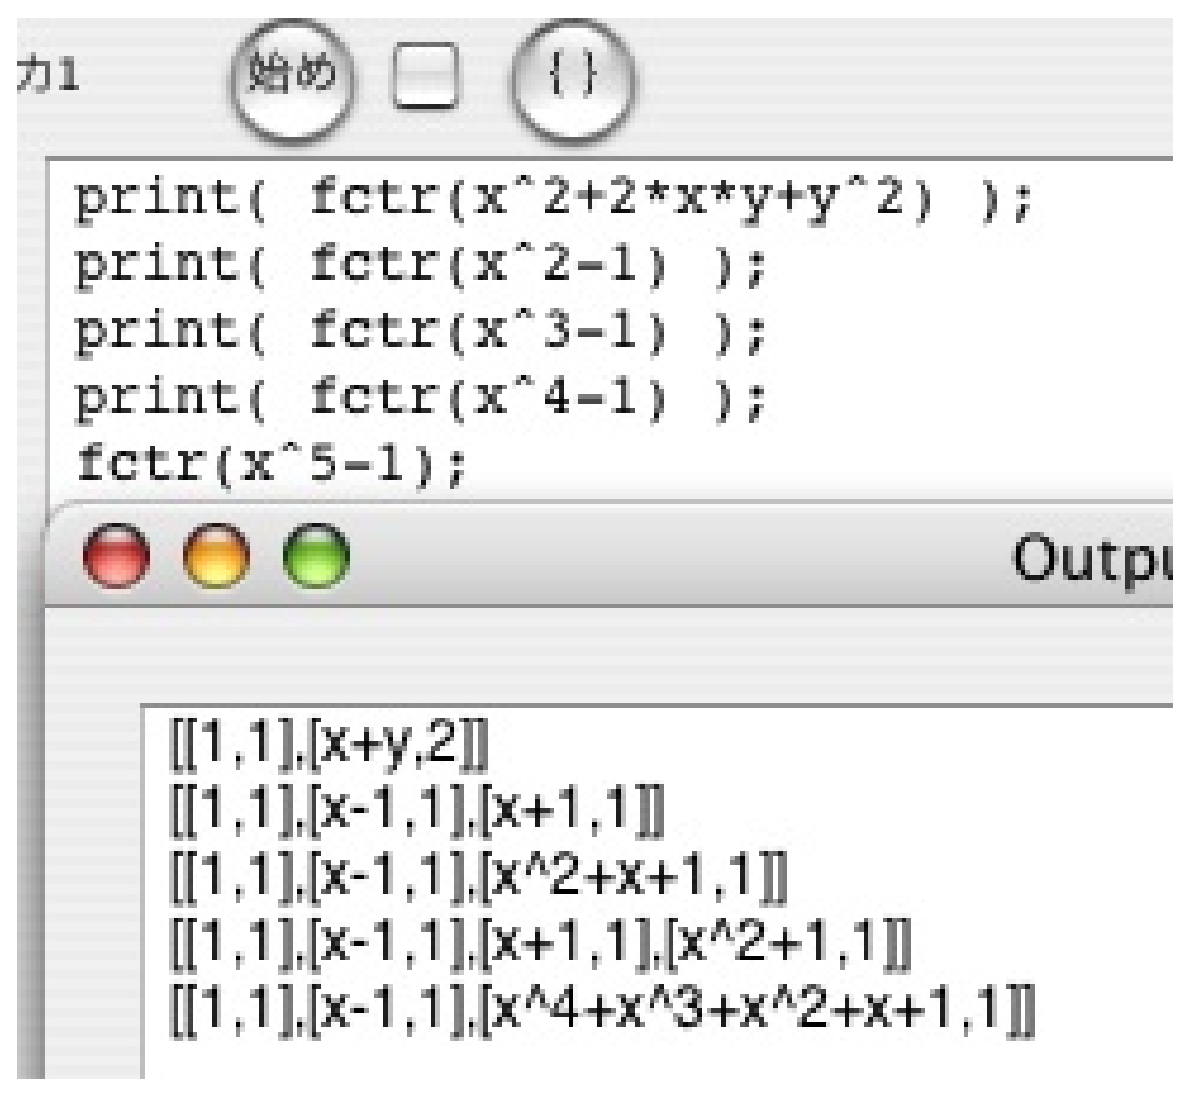
\includegraphics{Figs/fctr1.eps}}
\end{center}
\caption{$B0x?tJ,2r(B} \label{fig:fctr1}
\end{figure}

$B?^(B\ref{fig:fctr1} $B$N(B{\tt fctr} $B$N=PNO$N:G=i$O(B $x^2+2xy+y^2$ $B$,(B 
$ 1^1 \times (x+y)^2 $ 
$B$H0x?tJ,2r$5$l$k$3$H$r0UL#$7$F$$$k(B. 
$B?^(B\ref{fig:fctr1} $B$N(B{\tt fctr} $B$N=PNO$N(B2$BHVL\$O(B $x^2-1$ $B$,(B 
$$ 1^1 \times (x-1)^1 \times (x+1)^1 
$$ 
$B$H0x?tJ,2r$5$l$k$3$H$r0UL#$7$F$$$k(B. 


\section{$B$/$j$+$($7(B}

$B$/$j$+$($7$dH=CG$r$*$3$J$&$?$a$NJ8$,(B asir $B$K$OMQ0U$5$l$F$$$k(B.
$B$3$NJ8$r$b$A$$$k$HJ#;($J$3$H$r<B9T$G$-$k(B.
$B$^$:0lHV$N4pAC$G$"$k$/$j$+$($7$N5!G=$r$?$a$7$F$_$h$&(B.
\index{$B$/$j$+$($7(B} \index{for$B$V$s(B@for$BJ8(B}
%en A programming language is installed in Asir. 
%en Let us try the most basic programming; repeating and printing.
\begin{example} \rm
$B?^(B\ref{fig:powerOf2}$B$N%W%m%0%i%`$O<!$N$h$&$K7+$jJV$75!G=(B --- {\tt for}$BJ8(B ---
$B$rMQ$$$F4J7i$K=q$1$k(B.
\begin{screen}
\begin{verbatim}
  X = 2;
  for (I=1; I<=8; I++) {
     print( X^I );
  }
\end{verbatim}
\end{screen}
$B<B9T7k2L$O?^(B\ref{fig:powerOf2For}$B$r$_$h(B.
\end{example}

\begin{figure}[tbh]
\begin{center}
\scalebox{0.3}{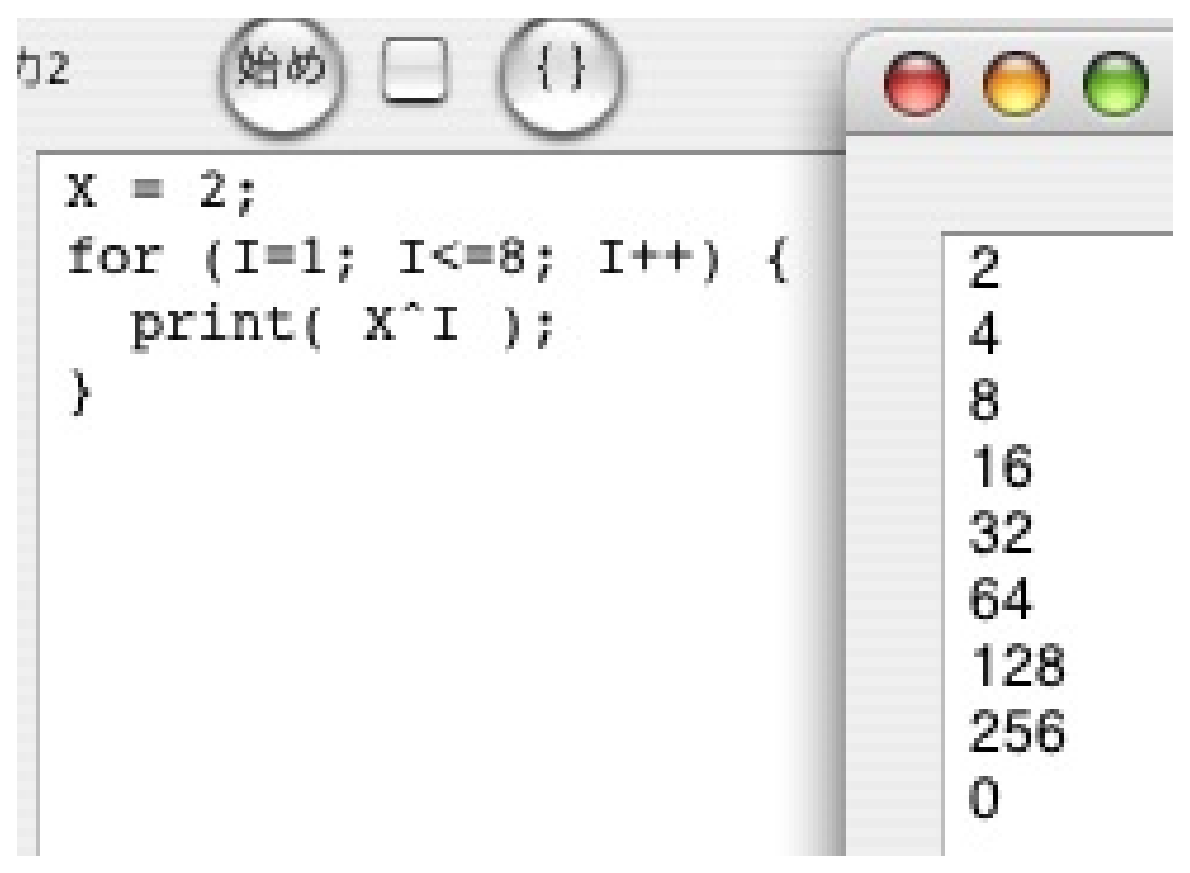
\includegraphics{Figs/powerOf2For.eps}}
\end{center}
\caption{for$BJ8(B} \label{fig:powerOf2For}
\end{figure}


$B7+$jJV$74XO"$NI=8=$N0UL#$r2U>r=q$K$7$F$^$H$a$F$*$3$&(B.
\begin{enumerate}
%en \begin{enumerate}
\item   \index{for} \index{$B$/$j$+$($7(B@$B7+$jJV$7(B} \index{\<@\verb&<=&}
%en \item   \index{for} \index{repeat} \index{\<@\verb&<=&}
\verb@ for (K=$B=i4|CM(B; K<=$B=*$j$NCM(B; K++) {$B%k!<%W$NCf$G<B9T$9$k%3%^%s%I(B}; @
$B$O$"$k$3$H$r2?EY$b7+$jJV$7$?$$;~$KMQ$$$k(B.
for $B%k!<%W$H8F$P$l$k(B.
``{\tt K<=N}'' $B$O(B, ``${\tt K} \leq {\tt N}$$B$+(B'' $B$H$$$&0UL#$G$"$k(B.
$B;w$?I=8=$K(B,
``{\tt K>=N}''$B$,$"$k$,(B, $B$3$l$O(B ``${\tt K} \geq {\tt N}$$B$+(B'' $B$H$$$&0UL#$G$"$k(B.
{\tt =} $B$N$J$$(B
``{\tt K<N}'' $B$O(B, ``${\tt K} < {\tt N}$$B$+(B'' $B$H$$$&0UL#$G$"$k(B.
\item \verb@ ++K @ $B$d(B \verb@ K++ @ $B$O(B {\tt K} $B$r(B 1 $BA}$d$;$H$$$&0UL#$G$"$k(B.
\verb@ K = K+1 @ $B$H=q$$$F$b$h$$(B.
$BF1$8$/(B, \verb@ --K @ $B$d(B \verb@ K-- @ $B$O(B {\tt K} $B$r(B 1 $B8:$i$;$H$$$&0UL#$G$"$k(B.
%en The sentence 
%en {\tt for (K={\it initial value}; K<={\it limit}; K++) \{{\it commands}\}; }
%en is used to repeat commands.
%en It is called the ``for'' loop.
%en ``{\tt K<=N}'' means that ``${\tt K} \leq {\tt N}$ holds''. 
%en A similar expression
%en ``{\tt K>=N}'' implies that ``${\tt K} \geq {\tt N}$ holds''
%en The expression ``{\tt K<N}'' means that ``${\tt K} < {\tt N}$''.
%en \item The expressions \verb@ ++K @ and \verb@ K++ @ mean increasing 
%en {\tt K} by $1$.
%en In this example, it has the same meaning with \verb@ K = K+1 @.
%en Similarly \verb@ --K @ and \verb@ K-- @ mean decreasing {\tt K} by 1.
%
%
\end{enumerate}
%en \end{enumerate}
%en

\begin{figure}[tbh]
\begin{center}
\scalebox{0.3}{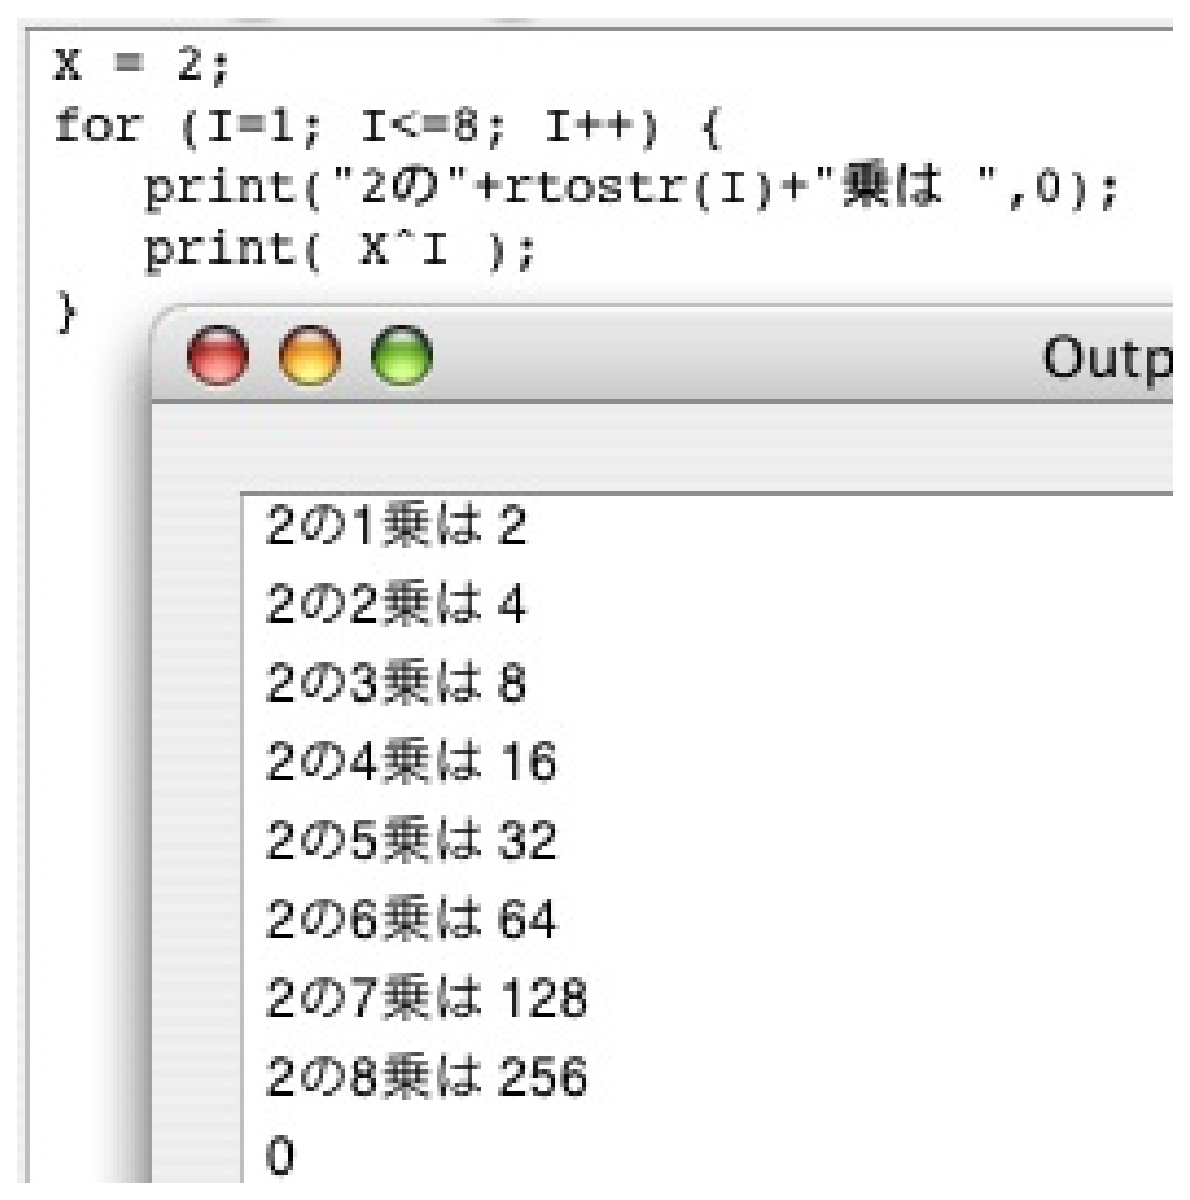
\includegraphics{Figs/powerOf2For2.eps}}
\end{center}
\caption{for$BJ8(B} \label{fig:powerOf2For2}
\end{figure}
for $B$N$"$H$N(B {\tt \{}, {\tt \}} $B$NCf$K$OJ#?t$NJ8(B($BL?Na(B)$B$r=q$1$k(B.
\begin{screen}
\begin{verbatim}
  X = 2;
  for (I=1; I<=8; I++) {
     print("2$B$N(B"+rtostr(I)+"$B>h$O(B ",0);
     print( X^I );
  }
\end{verbatim}
\end{screen}
$B$3$NNc$G$O(B  
$BF|K\8l$r4^$`$N$GA0$N@a$G=R$Y$?$h$&$KF|K\8l6uGr$r%W%m%0%i%`K\BN$K$$$l$J$$$h$&$K$7$F(B,
$BCm0U?<$/%W%m%0%i%`$rF~NO$7$F$b$i$$$?$$(B.  
$B<B9T7k2L$O?^(B\ref{fig:powerOf2For2}$B$r$_$h(B. \index{2$B$N$k$$$8$g$&(B@$2$$B$NN_>h(B}
\verb@print("2$B$N(B"+rtostr(I)+"$B>h$O(B ",0);@ $B$NItJ,$r4JC1$K@bL@$7$F$*$3$&(B.
$B$^$::G8e$N(B {\tt 0} $B$O=PNO$N$"$H2~9T$7$J$$(B, $B$D$^$j<!$N(B {\tt print} $BJ8$N=PNO$r(B
$B$=$N$^$^B3$1$h$H$$$&0UL#(B.   \index{print} \index{rtostr}
\verb@"@ $B$G$+$3$^$l$?ItJ,$OJ8;zNs$H8F$P$l$F$$$k(B.$B$3$l$O$3$N$^$^I=<($5$l$k(B.
\verb@rtostr(I)@ $B$O?t;z(B {\tt I} $B$rJ8;zNsI=8=$KJQ49$7$J$5$$(B, $B$H$$$&0UL#(B
($BD6F~Lg$H$7$F$OFq$7$$(B?).
$B$"$HJ8;zNs$KBP$7$F(B {\tt +} $B$rE,MQ$9$k$HJ8;zNs$,7k9g$5$l$k(B.
\index{$B$b$8$l$D$N$1$D$4$&(B@$BJ8;zNs$N7k9g(B}
\index{$B$b$8$l$D$R$g$&$2$s(B@$BJ8;zNsI=8=(B}


\noindent
\fbox{$B;(CL(B}
($B9>8M;~Be$N?t3X$NK\$K$"$C$?LdBj$N2~Bj(B) \\
$BEBMM(B: $B$3$N$?$S$NF/$-$O$"$C$Q$l$G$"$C$?(B. $BK+H~$O$J$K$,$h$$$+(B? \\
$B2HMh(B: $B:#F|$O0l1_(B, $BL@F|$O(B2$B1_(B, $BL@8eF|$O(B4$B1_$H(B, $BA0F|$N(B2$BG\$E$D(B, $B$3$l$r(B4$B=54VB3$1$F(B
$B$/$@$5$k$@$1$G7k9=$G$4$6$$$^$9(B. \\
$BEBMM(B: $B$J$s$H$b$5$5$d$+$JK+H~$8$c$N$&(B. $B$h$7$h$7(B. \\
$B$5$F(B, $B2HMh$O$$$/$iK+>^6b$r$b$i$($k$@$m$&(B?
$B$3$l$b$^$?(B$2$$B$NN_>h$N7W;;$G$"$k(B. \index{2$B$N$k$$$8$g$&(B@$2$$B$NN_>h(B}
Cfep/asir $B$G7W;;$7$F$_$h$&(B.



\begin{example}\Begin \quad
{\tt for} $B$K$h$k7+$jJV$7$rMQ$$$F(B $\sqrt{x}$ $B$N?tI=$r$D$/$m$&(B.
%en \begin{example}\Begin [02] \quad
%en By using {\tt for} loop, generate a table of  $\sqrt{x}$.
%en \end{example}
%en 
\begin{screen}
\begin{center}
\begin{verbatim}
  for (I=0; I<2; I = I+0.2) {
     print(I,0); print(" : ",0);
     print(deval(I^(1/2)));
  }
\end{verbatim}
\end{center}
\end{screen}
%>C
$B=PNO7k2L(B
%en Output.
%<C
\begin{center}
\begin{tabular}{|l|} \hline \sl
0 : 0 \\
0.2 : 0.447214 \\
0.4 : 0.632456 \\
0.6 : 0.774597 \\
0.8 : 0.894427 \\
1 : 1 \\
1.2 : 1.09545 \\
1.4 : 1.18322 \\
1.6 : 1.26491 \\
1.8 : 1.34164 \\
2 : 1.41421 \\
\hline 
\end{tabular}
\end{center}
%>C
\rm
\index{print}
{\tt print(A)} $B$OJQ?t(B {\tt A} $B$NCM$r2hLL$KI=<($9$k(B.
{\tt print($BJ8;zNs(B)} $B$OJ8;zNs$r2hLL$KI=<($9$k(B.
{\tt print(A,0)} $B$OJQ?t(B {\tt A} $B$NCM$r2hLL$KI=<($9$k$,(B, $BI=<($7$?(B
$B$"$H$N2~9T$r$7$J$$(B.
$B6uGr$bJ8;z$G$"$k(B.$B$7$?$,$C$F(B, $B$?$H$($P(B
{\tt A=10; print(A,0); print(A+1);} 
$B$r<B9T$9$k$H(B,   \index{print}
{\tt 1011} $B$HI=<($5$l$F$7$^$&(B.
{\tt A=10; print(A,0); print(" ",0);print(A+1);} 
$B$r<B9T$9$k$H(B,
{\tt 10 11} $B$HI=<($5$l$k(B.
%en \rm
%en \index{print}
%en The command {\tt print(A)} displays the value of the variable {\tt A}
%en on the screen.
%en The command {\tt print({\it string})} outpus the {\it string} on the screen.
%en The command {\tt print(A,0)} displays the value of the variable {\tt A},
%en but it does not make the newline.
%en Note that the blank is a character. For example, if you input
%en {\tt A=10; print(A,0); print(A+1);} 
%en {\tt 1011} will be displayed.   So, input as 
%en {\tt A=10; print(A,0); print(" ",0);print(A+1);} 
%en Then,
%en {\tt 10 11} will be displayed.
%en 
\end{example}

$B$H$3$m$G(B, $B$3$NNc$G$O>r7o$,(B ${\tt I}<2$ $B$J$N$K(B ${\tt I}=2$ 
$B$N>l9g$,I=<($5$l$F$$$k(B.
$B<B:]$K(B asir $B>e$G<B9T$7$F$_$k$H$3$&$J$k$,(B, $BM}M3$rCN$k$K$O!"(B
$BIbF0>.?t$N7W;;5!>e$G$NI=8=$K$D$$$F$NCN<1$,I,MW$G$"$k(B
(``asir$B%I%j%k(B''$B$r;2>H(B).
$B$H$j$"$($:(B, 
%en In this example, the termination condition is ${\tt I}<2$, but
%en the case of ${\tt I}=2$ is executed. In order to understand the reason,
%en we need to study the format of floating point numbers.
%en (See \ref{chapter:naibu} for details).
%en For now, please keep the following in our mind.
\begin{FRAME}
$B@0?t$dJ,?t$N7W;;$O(B Asir $B>e$G@53N$K<B9T$5$l$k$,(B,
$B>.?t$K$D$$$F$O$=$&$G$J$$(B. 
\end{FRAME}
$B$H3P$($F$*$3$&(B.
%en \begin{FRAME}
%en Arithmetics for integers and rational numbers are exact in Risa/Asir,
%en but arithmetics for dicimal numbers are not.
%en \end{FRAME}
%en 

\begin{problem}
  $B$"$?$($i$l$?(B 10 $B?J?t$r(B 2$B?J?t$XJQ49$9$k%W%m%0%i%`$r:n$l(B.
 $B%R%s%H(B: {\tt A}$B!`(B{\tt B} $B$NM>$j$O(B \verb@A%B@ $B$G7W;;$G$-$k(B.
  \index{$B$"$^$j(B@$BM>$j(B}
\end{problem}

\section{$B<B9T$NCf;_(B}
%
%
\index{$B$A$e$&$7(B@$BCf;_(B}  \index{interrupt}
$B<B9TCf$N7W;;$d%W%m%0%i%`$N<B9T$rCf;_$7$?$$;~$OCf;_%\%?%s(B
\begin{center}
\scalebox{0.1}{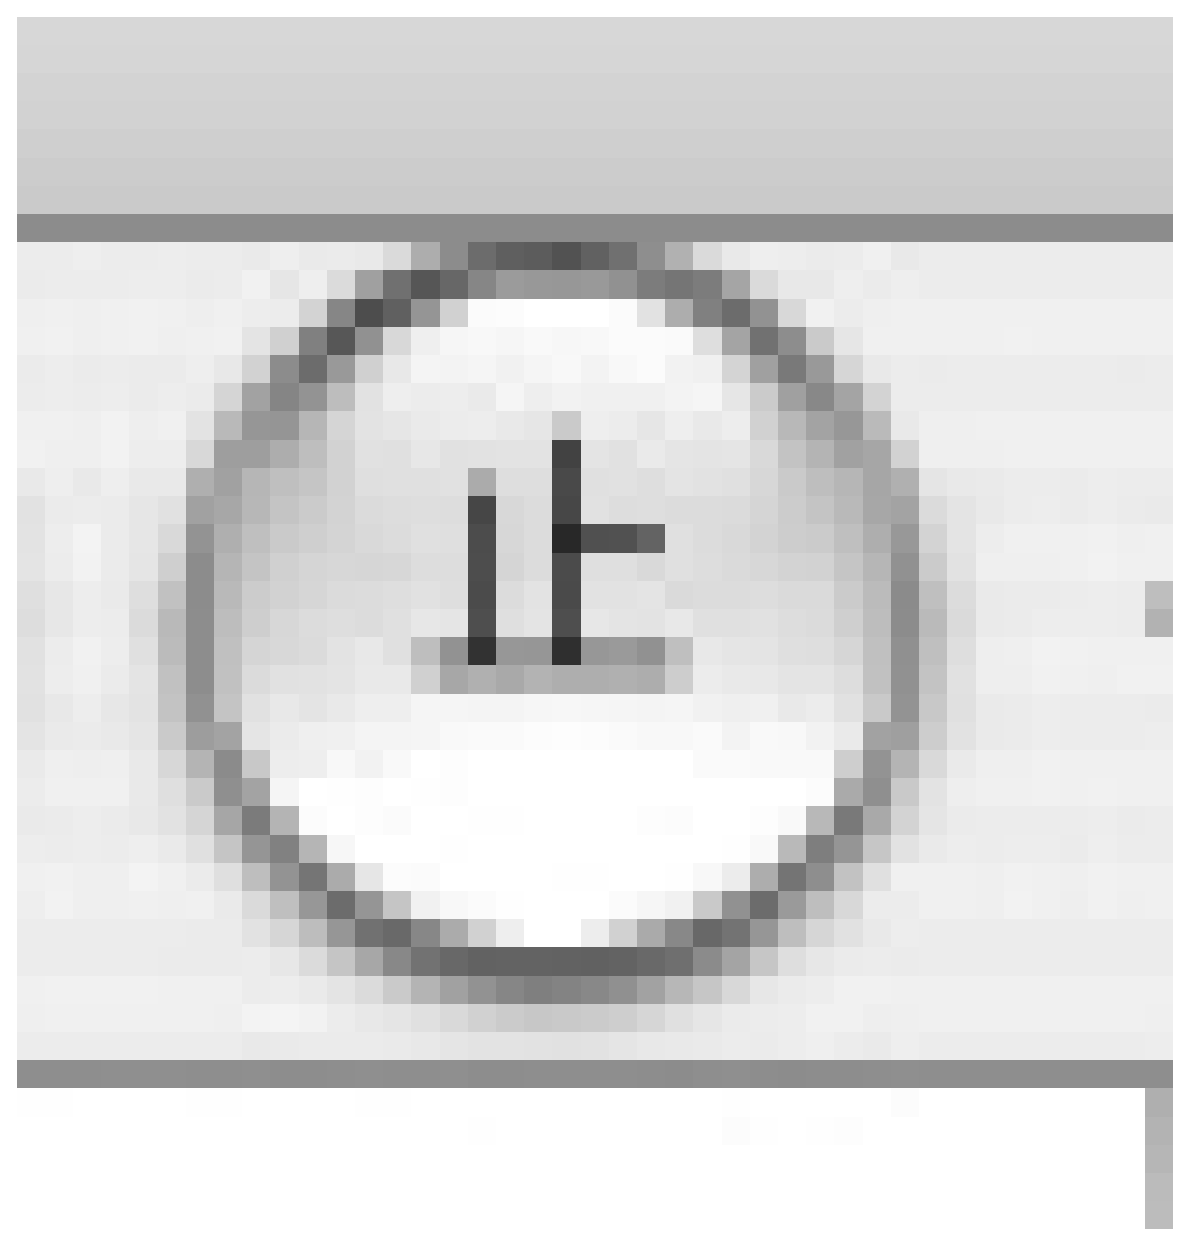
\includegraphics{Figs/buttonStop.eps}}
\end{center}
$B$r%/%j%C%/$9$k(B.

\begin{figure}[tbh]
\begin{center}
\scalebox{0.5}{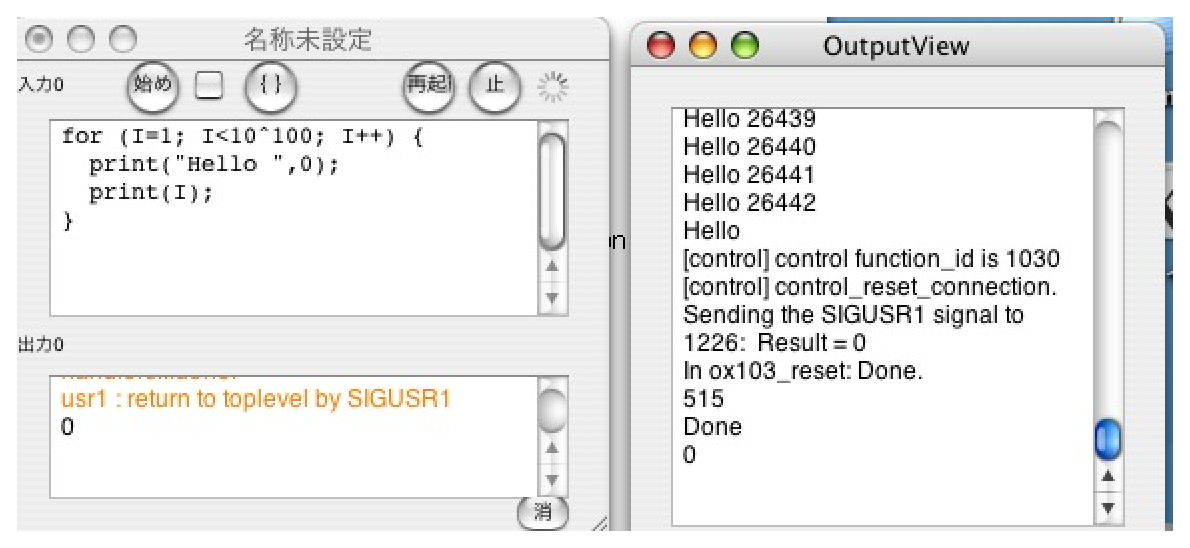
\includegraphics{Figs/interrupt.eps}}
\end{center}
\caption{$B<B9T$NCf;_(B} \label{fig:interrupt}
\end{figure}

$B?^(B\ref{fig:interrupt}$B$G$O(B
$10^{100}$ $B2s$N(B {\tt Hello } $B$N=PNO$N7+$jJV$7$rCf;_$7$F$$$k(B.

cfep $B$O3+H/ES>e$N%7%9%F%`$N$?$a(B
\begin{verbatim}
[control] control function_id is 1030
[control] control_reset_connection.
Sending the SIGUSR1 signal to 1226:  Result = 0
In ox103_reset: Done.
515
Done
\end{verbatim}
$B$3$N$h$&$J3+H/<T@lMQ$N%a%C%;!<%8$b=PNO$5$l$k$,(B,
$B$H$j$"$($:$3$N$h$&$J%a%C%;!<%8$,$G$?$iCf;_$,@.8y$7$?$H$$$&$3$H$G$"$k(B.


\section{$B%(%s%8%s:F5/F0(B}

\index{$B$5$$$-$I$&(B@$B:F5/F0(B}  \index{$B$1$$$5$s$($s$8$s(B@$B7W;;%(%s%8%s(B}
\index{$B$1$$$5$s$5!<$P(B@$B7W;;%5!<%P(B}
Cfep/asir $B$G$O<!$N$h$&$K(B3$B$D$N%W%m%;%9$,8_$$$KDL?.$7$J$,$iF0:n$7$F$$$k(B.
\begin{center}
\fbox{cfep} $\Leftrightarrow$ \fbox{$B%3%s%H%m!<%i(B(ox\_texmacs)}
$\Leftrightarrow$ \fbox{$B7W;;%(%s%8%s(B(ox\_asir)}
\end{center}
$B7W;;%(%s%8%s(B($B7W;;%5!<%P(B)$B$r:F5/F0$7$?$jJL$N$b$N$K$H$j$+$($?$j$G$-$k(B.
\index{$B$1$$$5$s$($s$8$s(B@$B7W;;%(%s%8%s(B}
\index{$B$1$$$5$s$5!<$P(B@$B7W;;%5!<%P(B}
\index{$B$($s$8$s(B@$B%(%s%8%s(B}

\index{$B$5$$$-$I$&(B@$B:F5/F0(B}  \index{restart}
$B%(%s%8%s:F5/F0%\%?%s(B
\begin{center}
\scalebox{0.05}{
\includegraphics{Figs/buttonRestart}}
\end{center}
$B$r%/%j%C%/$9$k$H(B,
$B8=:_MxMQ$7$F$$$k7W;;%(%s%8%s$rDd;_$7(B,
$B?7$7$$7W;;%(%s%8%s$r%9%?!<%H$9$k(B.
$BA*BrHO0O$N$_$r<B9T$9$k%b!<%I$G$J$$$+$.$jMxMQ>e$GCf;_$H$N0c$$$O(B
$B$"$^$j$J$$$,(B, $B:F5/F0$N$H$-$N%a%C%;!<%8(B
\begin{center}
\scalebox{0.4}{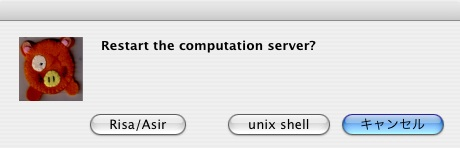
\includegraphics{Figs/restartDialog}}
\end{center}
$B$K$b$"$k$h$&$K(B, $BJL$N7W;;%(%s%8%s$r5/F0$9$k$3$H$b2DG=$G$"$k(B.
$B$3$NNc$G$O(B unix shell $B$b5/F0$G$-$k(B.

$B$^$?(B, ``$B<B9T(B'' $B%a%K%e!<$+$i(B ``$B%(%s%8%s$r<+F0%9%?!<%H$7$J$$(B'' $B%b!<%I$rA*$s$G$k(B
$B>l9g$K7W;;%(%s%8%s$r<jF0$G%9%?!<%H$9$k$K$O(B, $B$3$N%\%?%s$rMQ$$$k(B.

\bigbreak

\noindent
\HHH
cfep $B$O(B  \index{cfep}
Cocoa FrontEnd view Process 
$B$NN,$G$"$k(B.
cfep $B$O(B Objective C $B$H$$$&8@8l$*$h$S(B xcode 2 $B$H$$$&3+H/4D6-$rMQ$$$F(B
Cocoa $B$H$$$&%U%l!<%`%o!<%/$N$b$H$G3+H/$5$l$F$$$k(B.
cfep $B$N(B Objective C $B$N%W%m%0%i%`$N0lIt$r$_$F$_$h$&(B.
\begin{screen}
\begin{verbatim}
  for (i=0; i<oglCommSize; i++) {
    gc = [oglComm objectAtIndex: i];
    [self execute: gc];
  }
\end{verbatim}
\end{screen}
asir $B$HF1$8$h$&$J(B {\tt for} $BJ8$,$"$k$M(B.

\section{$B%X%k%W$NMxMQ(B}

\index{$B$+$s$9$&(B@$B4X?t(B}
Cfep/asir $B$G$N(B ``$B4X?t(B'' $B$H$O?t3X$N4X?t$N$h$&$K0z?t$rM?$($k$H7W;;$7$FCM$r$b$I$7(B,
$B$+$D$"$k;E;v(B($BI=<(Ey(B)$B$r$9$k<jB3$-$N=8$^$j$G$"$k(B.
$BNc$($P(B {\tt print}, {\tt deval}, {\tt sin}, {\tt fctr} $BEy$O4X?t$G$"$k(B.
$B4X?t$r<+J,$GDj5A$9$k$3$H$b2DG=$G$"$k(B. $B$3$l$K$D$$$F$O8e$N@bL@$*$h$S(B
``asir$B%I%j%k(B''$B$r;2>H(B.

$B$"$i$+$8$aDj5A$:$_$N4X?t$r(B ``$BAH$_9~$_4X?t(B'' $B$H$h$V(B.
\index{help}  
\index{$B$X$k$W(B@$B%X%k%W(B}  \index{$B$/$_$3$_$+$s$9$&(B@$BAH$_9~$_4X?t(B}
$BAH$_9~$_4X?t$N>\$7$$@bL@$rD4$Y$k$K$O(B
``cfep $B$N%X%k%W(B'' $B$+$i(B
\begin{center}
\scalebox{0.3}{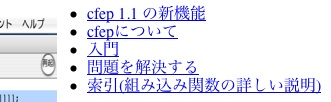
\includegraphics{Figs/helpTop}}
\end{center}
$B$N(B ``$B:w0z(B'' $B$rA*$S(B, $B:w0z(B
\begin{center}
\scalebox{0.45}{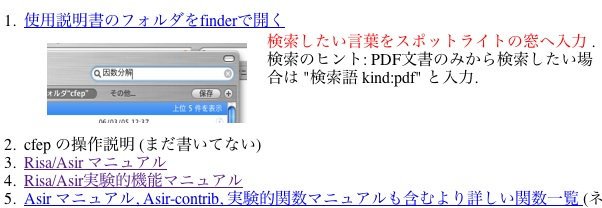
\includegraphics{Figs/helpIndex}}
\end{center}
$B$N(B ``Risa/Asir $B%^%K%e%"%k(B'' $B$rA*$S(B,
``Risa/Asir $B%^%K%e%"%k(B'' $B$N:G=i$N%Z!<%8$N4X?t0lMw$+$i(B
$BD4$Y$?$$4X?t$rC5$9(B.
$B$?$H$($P(B {\tt fctr} ($B0x?tJ,2rMQ$N4X?t(B) $B$O$3$N0lMw$NCf$K$"$k(B.
\begin{center}
\scalebox{0.35}{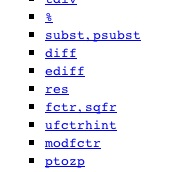
\includegraphics{Figs/helpFctr}}
\end{center}
\index{fctr}


\index{spotlight}
$B8!:w$K$O(B spotlight $B$N3hMQ$bM-1W$G$"$m$&(B. $B:w0z(B
\begin{center}
\scalebox{0.45}{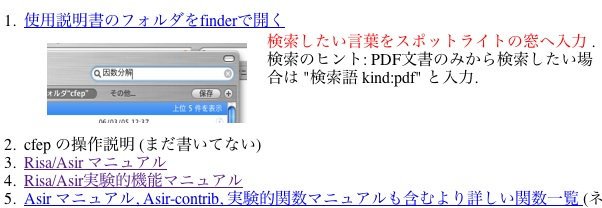
\includegraphics{Figs/helpIndex}}
\end{center}
$B$N(B ``$B;HMQ@bL@=q$N%U%)%k%@$r(Bfinder$B$G3+$/(B''
$B$rA*$V$H;HMQ@bL@=q$N%U%)%k%@$,3+$/$N$G(B, $B$3$3$r(B spotlight $B$G8!:w$9$k$H(B
$B$$$m$$$m$JH/8+$,$"$k$G$"$m$&(B.
$B$A$J$_$K(B, $B$3$ND6F~Lg$d(B asir$B%I%j%k$O$3$N%U%)%k%@$N(B pdf $B%U%)%k%@$NCf$K$"$k(B.
($B$J$*$3$3$+$i$N(B spotlight $B8!:w$O2?8N$+CY$$$N$G(B, $B%a%K%e!<%P!<$N(B 
 splotlight $B$+$i$N8!:w$NJ}$,$$$$$+$b$7$l$J$$(B.
)
%% mdfind, mdimport?


\chapter{$B%0%i%U%#%C%/(B}

\section{$B%i%$%V%i%j$NFI$_9~$_(B}  \index{$B$i$$$V$i$j(B@$B%i%$%V%i%j(B}

\begin{figure}
\begin{center}
\scalebox{0.5}{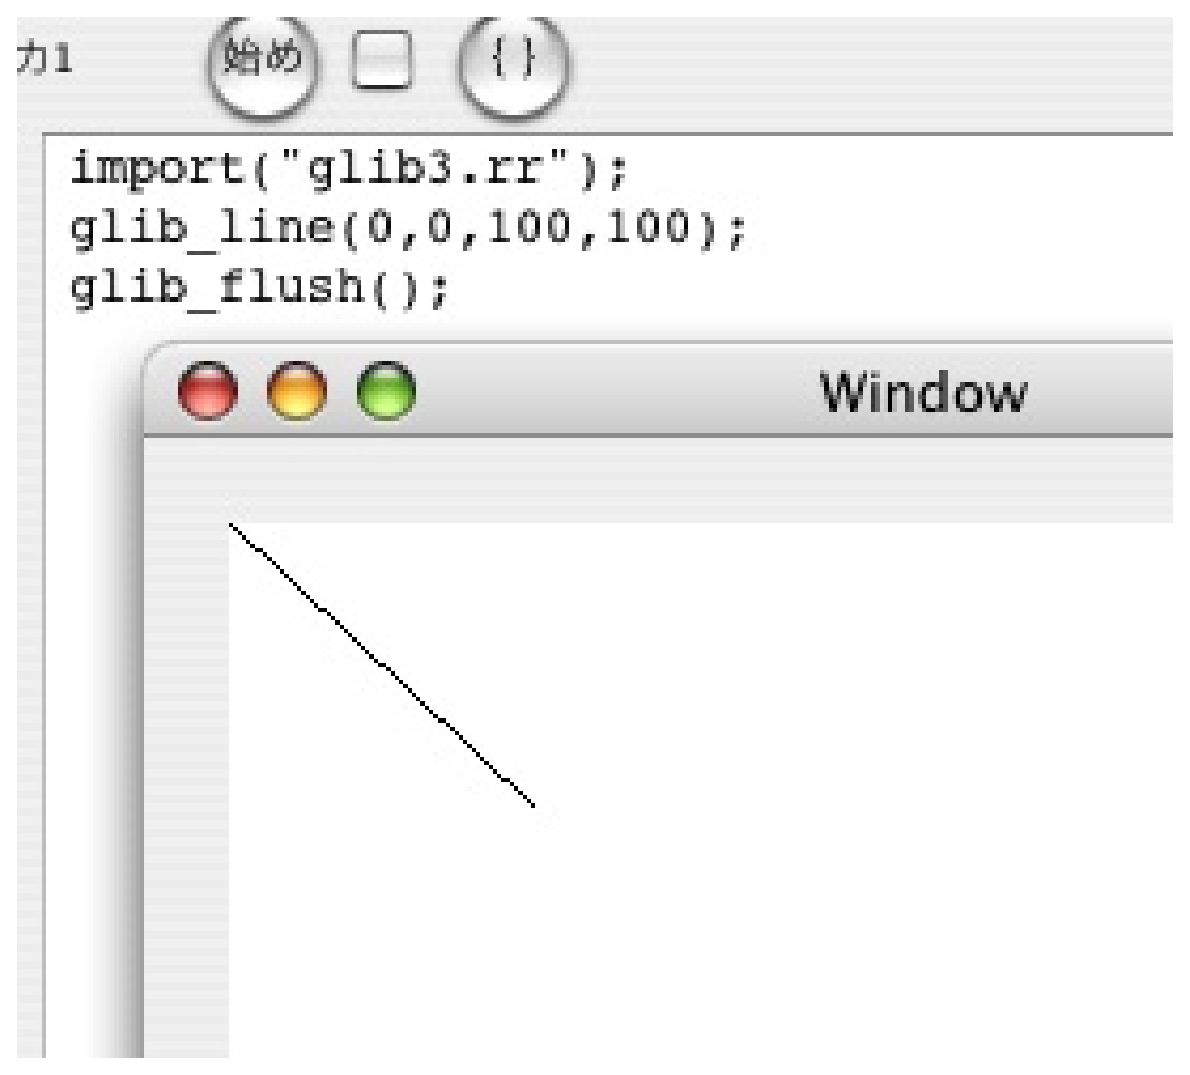
\includegraphics{Figs/glib_lineImport.eps}}
\end{center}
\caption{$B%i%$%V%i%j$N%m!<%I(B} \label{fig:glib_lineImport}
\end{figure}

Asir $B8@8l$G=q$+$l$F$$$k4X?tDj5A$N=89g$,%i%$%V%i%j$G$"$k(B.
$B%i%$%V%i%j$rFI$_9~$`$K$O(B {\tt import} $B%3%^%s%I$^$?$O(B
{\tt load} $B%3%^%s%I$rMQ$$$k(B.   \index{import}  \index{load}
$B%^%K%e%"%k$K5-=R$5$l$F$$$k4X?t$G%i%$%V%i%j$NFI$_9~$_$,A0Ds$H$J$C$F$k$b$N$b(B
$BB?$$(B.
$B$?$H$($P(B, $B@~$r0z$/%3%^%s%I(B {\tt glib\_line(0,0,100,100);} 
$B$r<B9T$7$F$b(B, ``glib\_line $B$,Dj5A$5$l$F$$$^$;$s(B''
$B$H$$$&%(%i!<$,I=<($5$l$k(B.
$B%0%i%U%#%C%/%3%^%s%I$N%i%$%V%i%jFI$_9~$`%3%^%s%I(B
\begin{verbatim}
  import("glib3.rr");
\end{verbatim}
$B$r<B9T$7$F$*$/$H?^(B\ref{fig:glib_lineImport}$B$N$h$&$K(B
$B@~$rIA2h$9$k(B.


Asir-contrib $B%W%m%8%'%/%H$K$h$j=8@Q$5$l$?%i%$%V%i%j$N=89gBN$,(B
asir-contrib $B$G$"$k(B.  \index{asir-contrib}
Asir-contrib $B$rFI$_9~$s$G$7$^$&$H(B,
$B$[$H$s$I$N4X?t$K$D$$$F(B import $B$,I,MW$+$I$&$+5$$K$9$kI,MW$O$J$/$J$k$,(B,
$BBgNL$N%i%$%V%i%j$rFI$_9~$`$?$a$K;~4V$,$+$+$k$N$,7gE@$G$"$k(B.
asir-contrib $B$O(B \fbox{$B<B9T(B} $B%a%K%e!<$+$iFI$_9~$a$k(B.
\begin{center}
\scalebox{0.3}{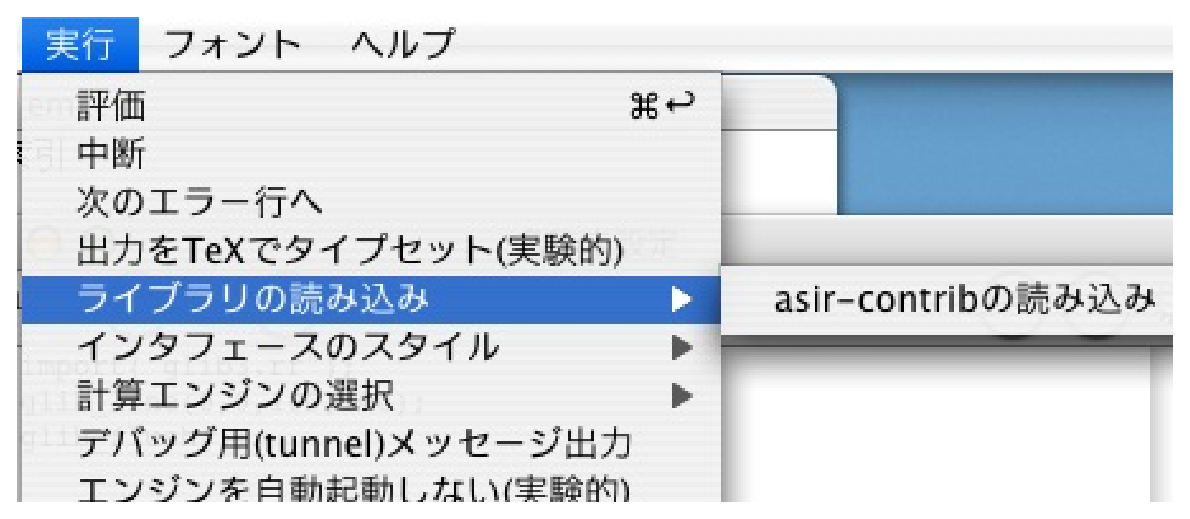
\includegraphics{Figs/importContrib}}
\end{center}

\section{$B@~$r0z$/4X?t(B}

\begin{example} \rm
\begin{screen}
\begin{verbatim}
   import("glib3.rr");
   glib_line(0,0, 100,100);
   glib_flush();
\end{verbatim}
\end{screen}
$B?^(B\ref{fig:glib_lineImport} $B$,IA2h7k2L$G$"$k(B.
$y$$B:BI8$O2hLL$,2<$X$$$/$[$IBg$-$/$J$k(B.
$B?^(B\ref{figure:cond:coord} $B$r;2>H(B.
$B:8>e$N:BI8$O(B $(0,0)$, $B1&2<$N:BI8$,(B $(400,400)$.
\verb@glib_line@ $B$G(B $(0,0)$ $B$+$i(B $(100,100)$ $B$X@~$rIA2h(B.
\verb@glib_flush@ $B$O2hLL$r99?7$9$k$O$?$i$-$,$"$k(B. flush $B$7$J$$$H(B,
$BIA2h7k2L$,2hLL$G$NI=<($KH?1G$7$J$$>l9g$,$"$k(B.
\end{example}

\index{glib}
{\tt glib3.rr} $B$r%m!<%I$9$k$3$H$K$h$j(B, $B<!$N4X?t$,;H$($k$h$&$K$J$k(B. \\
\begin{tabular}{|l|l|} 
\hline
{\tt glib\_window(X0,Y0,X1,Y1)} &  
                            $B?^$r=q$/(B window $B$N%5%$%:$r7h$a$k(B. \\ 
 & $B2hLL:8>e$N:BI8$,(B {\tt (X0,Y0)},
   $B2hLL1&2<$N:BI8$,(B {\tt (X1,Y1)} \\
 & $B$G$"$k$h$&$J:BI87O$G0J2<IA2h$;$h(B. \\ 
& $B$?$@$7(B x $B:BI8$O(B, $B1&$K$$$/$K=>$$$*$*$-$/$J$j(B, \\
&
  y $B:BI8$O(B \underline{$B2<$K(B} $B$$$/$K=>$$Bg$-$/$J$k(B ($B?^(B \ref{figure:cond:coord}).  \\ \hline
{\tt glib\_clear()} &  $BA4$F$N(BOpenGL$B%*%V%8%'%/%H$r>C5n$7(B,
                          $BIA2h2hLL$r%/%j%"$9$k(B. \\ \hline
{\tt glib\_putpixel(X,Y)} &  $B:BI8(B {\tt (X,Y)} $B$KE@$rBG$D(B. \\ \hline
{\tt glib\_set\_pixel\_size(S)} &  
   $BE@$NBg$-$5$N;XDj(B.  1.0 $B$,(B1$B%T%/%;%kJ,$NBg$-$5(B. \\ \hline
{\tt glib\_line(X,Y,P,Q)} &  $B:BI8(B {\tt (X,Y)} $B$+$i(B $B:BI8(B {\tt (P,Q)} $B$XD>@~$r0z$/(B \\ \hline
{\tt glib\_remove\_last()} & $B0l$DA0$N(B OpenGL $B%*%V%8%'%/%H$r>C$9(B.  \\ \hline
\end{tabular}

\begin{figure}[htb]  
\setlength{\unitlength}{1mm}
\begin{picture}(100,40)(0,0)
\put(20,35){\vector(1,0){80}}
\put(98,32){x}
\put(20,35){\vector(0,-1){35}}
\put(23,1){y}
\end{picture}
\caption{$B:BI87O(B}  \label{figure:cond:coord}
\end{figure}

$B?'$rJQ99$7$?$$$H$-$O(B,  \verb@ | @ $B5-9f$G6h@Z$C$?%*%W%7%g%J%k0z?t(B
{\tt color} $B$r;H$&(B.  \index{$B$*$W$7$g$J$k$R$-$9$&(B@$B%*%W%7%g%J%k0z?t(B}
$B$?$H$($P(B,
\begin{center}
\verb@ glib_line(0,0,100,100|color=0xff0000); @
\end{center}
$B$HF~NO$9$k$H(B, $B?'(B {\tt 0xff0000} $B$G@~J,$r$R$/(B.
$B$3$3$G(B, $B?'$O(B RGB $B$N3F@.J,$N6/$5$r(B 2 $B7e$N(B 16 $B?J?t$G;XDj$9$k(B.
16$B?J?t$K$D$$$F$O(B ``asir $B%I%j%k(B'' $B$r;2>H(B.
$B$3$NNc$G$O(B, R $B@.J,$,(B ff $B$J$N$G(B, $B@V$N@~$r$R$/$3$H$H$J$k(B.
$B$J$*(B, $B4X?t(B {\tt glib\_putpixel} $B$bF1$8$h$&$K$7$F(B, $B?'$r;XDj$G$-$k(B.
16$B?J?t$rCN$i$J$$?MMQ$K(B, $B?'$H$=$N(B16$B?J?t$K$h$kI=8=$NBP1~I=$r$"$2$F$*$/(B.

\begin{tabular}{|l|l|}
\hline 
0xffffff  & $BGr(B \\ \hline 
0xffff00  & $B2+(B \\ \hline
0xff0000  & $B@V(B \\ \hline
0x00ff00  & $BNP(B \\ \hline 
0x0000ff  & $B@D(B \\ \hline 
0x000000  & $B9u(B \\ \hline 
\end{tabular}

\noindent
($B$"$H$O;n$7$F2<$5$$(B)

$B$5$F(B, $B?^(B \ref{figure:cond:coord} $B$G8+$?$h$&$K%3%s%T%e!<%?%W%m%0%i%`$N(B
$B@$3&$G$O(B, $B2hLL$N:8>e$r86E@$K$7$F(B, $B2<$X$$$/$K=>$$(B, $y$ $B:BI8$,A}$($k$h$&$J(B
$B:BI87O$r$H$k$3$H$,B?$$(B.
$B?t3X$N%0%i%U$r=q$$$?$j$9$k$K$O$3$l$G$OITJX$J$3$H$bB?$$$N$G(B,
{\tt glib3.rr} $B$G$O(B,
\begin{center}
  \verb@ Glib_math_coordinate=1; @
\end{center}
$B$r<B9T$7$F$*$/$H(B 
$B2hLL$N:82<$,86E@$G(B, $B>e$K$$$/$K=>$$(B $y$ $B:BI8$,A}$($k$h$&$J(B
$B?t3X$G$N:BI87O$G?^$rIA2h$9$k(B.

\begin{example} \rm   \index{$B$0$i$U(B@$B%0%i%U(B}
2$B<!4X?t(B $y=x^2-1$ $B$N%0%i%U$r=q$$$F$_$h$&(B.
%%Prog: cfep/tests/2006-03-11-graph2d.rr
\begin{screen}
\begin{verbatim}
import("glib3.rr");
Glib_math_coordinate=1;
glib_window(-2,-2, 2,2);

glib_line(-2,0,2,0 | color=0x0000ff);
glib_line(0,-2,0,2 | color=0x0000ff);
for (X=-2.0; X< 2.0; X = X+0.1) {
   Y = X^2-1;
   X1 = X+0.1;
   Y1 = X1^2-1;
   glib_line(X,Y, X1,Y1);
}
glib_flush();
\end{verbatim}
\end{screen}
$B<B9T7k2L$O?^(B\ref{fig:graph2d}.
-----$B%W%m%0%i%`$N2r@b$O$^$@=q$$$F$J$$(B.
\end{example}

%<C
\begin{figure}[tb]
\scalebox{0.6}{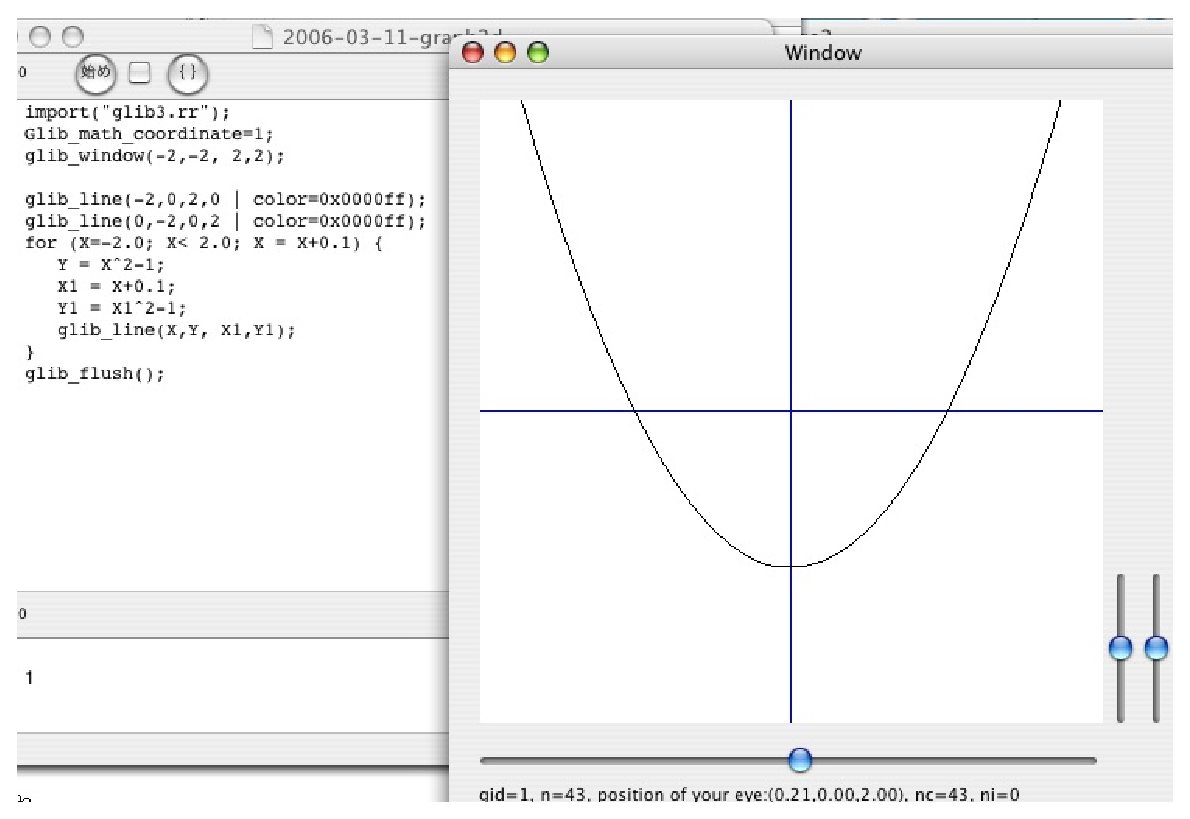
\includegraphics{Figs/graph2d.eps}}
\caption{2$B<!4X?t$N%0%i%U(B} \label{fig:graph2d}
\end{figure}
%>C


\section{$B1_$rIA$/4X?t$r:n$C$F$_$h$&(B}

%%Prog: cfep/tests/2006-03-11-circle.rr
\begin{screen}
\begin{verbatim}
import("glib3.rr");
Glib_math_coordinate=1;
glib_window(-1,-1,1,1);
glib_clear();
E = 0.2;  X = 0; Y = 0;  R = 0.5;
for (T=0; T<=deval(2*@pi); T = T+E) {
  Px = X+deval(R*cos(T));
  Py = Y+deval(R*sin(T));
  Qx = X+deval(R*cos(T+E));
  Qy = Y+deval(R*sin(T+E));
  glib_line(Px,Py,Qx,Qy);
  glib_flush(); 
}
\end{verbatim}
\end{screen}
-----$B%W%m%0%i%`$N2r@b$O$^$@=q$$$F$J$$(B.

$B>e$N%W%m%0%i%`$G$O(B $\cos$, $\sin$ $B$rMQ$$$F1_$rIA$$$F$$$k(B.
$BCf?4(B, $BH>7B$rJQ99$7$?$j(B, $B?'$rJQ99$7$?$j$7$J$,$i$?$/$5$s$N1_$rIA$/$K$O(B,
$B$I$N$h$&$K$9$l$P$h$$$G$"$m$&$+(B?
``$B4X?t(B'' $B$rMQ$$$k$H$=$l$,MF0W$K$G$-$k(B.

$B$"$k$R$H$^$H$^$j$N%W%m%0%i%`$O4X?t(B (function) $B$H$7$F(B
$B$^$H$a$F$*$/$H$h$$(B.   \index{$B$+$s$9$&(B@$B4X?t(B} 
$B7W;;5!8@8l$K$*$1$k4X?t$O?t3X$G$$$&4X?t$H;w$FHs$J$k$b$N$G$"$k(B.
$B4X?t$r<jB3$-(B (procedure) $B$H$+(B $B%5%V%k!<%A%s(B (subroutine) $B$H$+(B
$B$h$V8@8l$b$"$k(B.
$B4X?t$rMQ$$$k:GBg$NMxE@$O(B, $B4X?t$r0lC6=q$$$F$7$^$($P(B,
$BCf?H$r%V%i%C%/%\%C%/%9$H$7$F07$($k$3$H$G$"$k(B.
$BBg5,LO$J%W%m%0%i%`$r=q$/$H$-$OJ#;($J=hM}$r$$$/$D$+$N4X?t$KJ,3d$7$F(B
$B$^$:3F4X?t$r==J,%F%9%H$7;E>e$2$k(B.
$B$=$l$+$i$=$l$i$N4X?t$rAH$_9g$o$;$F$$$/$3$H$K$h$j(B, 
$BJ#;($J5!G=$r<B8=$9$k(B.
$B$3$N$h$&$J%"%W%m!<%A$r$H$k$3$H$K$h$j(B, ``$B:$Fq$,J,3d(B'' $B$5$l$k(B.

$B1_$NNc$r$7$P$i$/N%$l(B,
$B4JC1$J4X?t$NNc$r$H$j4X?t$N=q$-J}$r@bL@$7$h$&(B.
$BA0$N@a$G$O(B $2$ $B$N6R$NI=$r:n@.$9$k%W%m%0%i%`$r=q$$$?(B.
$B$3$l$r85$K<!$N$h$&$J4X?t$r:n$k(B.
\begin{screen}
\begin{verbatim}
def power_table(N) {
  X=2;
  for (I=1; I<=N; I++) {
    print(X^I);
  }
}
power_table(8);
\end{verbatim}
\end{screen}
$B4X?t$NDj5A$O<!$N$h$&$K(B {\tt def} $BL?Na$G9T$J$&(B.
\begin{verbatim}
def  $B4X?tL>(B($B0z?t(B) {
  $B4X?tK\BN(B 
}
\end{verbatim}
$B>e$NNc$G$O4X?tL>$O(B {\tt power\_table} $B$G$"$j(B, $B0z?t(B(argument)$B$O(B {\tt N} $B$G$"$k(B.
$B4X?tL>$O1Q?t;z$H(B {\tt \_} $B$rMQ$$$F$D$1$k(B.
$B$?$@$7?t;z$dBgJ8;z$G$O$8$^$kL>A0$r$D$1$k$3$H$O$G$-$J$$(B.
$B=hM}FbMF$rO"A[$5$;$k$h$&$JL>A0$r$D$1$k$N$,K>$^$7$$(B.
{\tt def} $BL?Na$G$O4X?t$rDj5A$9$k$@$1$G<B9T$O9T$J$o$J$$(B.
$B<B9T$5$;$k$K$O(B, $B>e$NNc$N$h$&$K(B {\tt power\_table(8);} $B$H0z?t$NItJ,$K<B:]$N?t;zEy$rF~$l$F(B
$B8F$S=P$9(B.

$B0z?t$OFs$D0J>e$"$C$F$b$h$/$F(B,$B$?$H$($P(B,
\begin{screen}
\begin{verbatim}
def power_table2(X,N) {
  for (I=1; I<=N; I++) {
    print(X^I);
  }
}
power_table2(3,8);
\end{verbatim}
\end{screen}
$B$J$k4X?tDj5A$H:G8e$N9T$N$=$N8F$S=P$7$O(B 
$3^i$ $B$r(B $i=1, \ldots, 8$ $B$NHO0O$G7W;;$7$FI=<($9$k(B.
$B$3$N$h$&$J4X?t$rMQ0U$7$F$*$1$P(B,
$2^i$, $3^i$, $5^i$, $1 \leq i \leq 10$ $B$NI=$rI=<($7$?$$$H$9$k$H(B,
\begin{screen}
\begin{verbatim}
power_table2(2,10);
power_table2(3,10);
power_table2(5,10);
\end{verbatim}
\end{screen}
$B$H=q$/$@$1$GNI$/(B, $B%W%m%0%i%`$bC;$/$J$j(B, $B$+$D@0M}$5$l$F$$$k$N$G(B, $BFI$_$d$9$/$J$k(B.

$B$5$F(B, {\tt power\_table2(2,3);} $B$r<B9T$9$k$H(B
\begin{screen}
\begin{verbatim}
2
4
8
0
\end{verbatim}
\end{screen}
$B$HI=<($5$l$k(B. 
$B:G8e$N(B 0 $B$O0lBN2?$G$"$m$&$+(B?
$B$3$l$O<B$O4X?t$NCM$G$"$k(B. 
$B4X?t$NCM$N$3$H$rLa$jCM$H$b$$$&(B.
$BLaCM$r;XDj$9$k$K$O(B, {\tt return} $BJ8$rMQ$$$k(B.
\begin{flushleft}
\begin{minipage}[t]{7cm}
\begin{screen}
\begin{verbatim}
def twotimes(N) {
  S=2*N;
  return(S);
}
\end{verbatim}
\end{screen}
\end{minipage} \quad
%
\begin{minipage}[t]{7cm}
$B4X?t(B {\tt twotimes(N)} $B$O(B
$2N$ $B$NCM$r7W;;$7$FLa$9(B. \\
$B$3$NDj5A$r=q$$$F$*$$$F(B
\begin{verbatim}
A=twotimes(10);
B=twotimes(100);
print(A+B);
\end{verbatim}
$B$r<B9T$9$k$H(B, {\tt A} $B$K$O(B $20$ $B$,BeF~$5$l(B, {\tt B} $B$K$O(B $200$ $B$,BeF~$5$l(B,
{\tt print}$BJ8$K$h$j(B $220$ $B$,=PNO$5$l$k(B.
$B$=$N$"$H(B $0$ $B$,=PNO$5$l$k$,$3$l$O(B {\tt print}$BJ8$NLa$jCM$G$"$k(B.
\end{minipage} \\
\end{flushleft}

\noindent  
$B4X?t$NLa$jCM(B (return value) $B$O(B {\tt return} $BJ8$G(B
$B;XDj$9$k(B.
$B$$$^$N>l9g$OJQ?t(B {\tt S} $B$NCM$G$"$k(B.
$B$J$*(B, {\tt print} $B$H(B {\tt return}  $B$O0c$&(B.
{\tt print} $B$O2hLL$KCM$r0u:~$9$k$N$KBP$7$F(B,
{\tt return} $B$O4X?t$NCM$rLa$9F/$-$r;}$D(B.
{\tt print} $BJ8$G$O(B, $B4X?t$NCM$rLa$9$3$H$O$G$-$J$$(B.

``$BLa$jCM(B''(return value) $B$H$$$&8@$$J}$O7W;;5!8@8lFCM-$N8@$$$^$o$7$G$"$k(B.
``$B4X?t(B {\tt twotimes} $B$O0z?t$N(B2$BG\$r7W;;$7$F7k2L$rLa$9(B'' $B$_$?$$$K;H$&(B.
$B>e$NNc$G$$$($P(B {\tt A=twotimes(10)} $B$H$7$?$H$-(B,
$BLa$jCM$,4X?t$NCM$H$7$FJQ?t(B {\tt A} $B$KBeF~$5$l$k(B.


$B4X?t$N$J$+$GMxMQ$5$l$F$$$kJQ?t$H0z?t$O(B,
$B$=$N4X?t$N<B9TCf$N$_@8@.$5$l$kJQ?t$G$"$j(B,
$B$5$i$K$=$N4X?t30It$NF1L>$NJQ?t$NCM$rJQ$($J$$(B.
$B$3$N$h$&$K0l;~E*$K@8@.$5$l$kJQ?t$r6I=jJQ?t(B (local variable) $B$H$h$V(B.
$B4X?t$NCf$GJQ?t$NCM$rJQ99$7$?$i(B, $B$=$N4X?t$N30$NF1$8L>A0$NJQ?t$N(B
$BCM$b$+$o$C$F$7$^$&$H$7$?$i(B, $B=hM}$rJ,3d$7$?MxE@$,$9$/$J$$(B.
$B$=$3$G$G$F$-$?35G0$,$3$N(B ``$B6I=jJQ?t(B''
$B$N35G0$G$"$k(B.
$B>e$N%W%m%0%i%`Nc$G$O(B,
{\tt N}, {\tt S} $B$,6I=jJQ?t$G$"$k(B.
$B6I=jJQ?t$O$=$N4X?t$N$J$+$@$1$GM-8z$JJQ?t$G$"$k(B.
$B$3$l$r(B, ``$B6I=jJQ?t$N%9%3!<%W$O$=$N4X?t$N$J$+$@$1(B'' $B$H$$$&(B
$B8@$$$+$?$r$9$k(B. 
$B6I=jJQ?t$N9M$(J}$O(B, $B7W;;5!8@8l$NNr;K$G$OBgH/L@$N0l$D$G$"$k(B.

\noindent
$BNc(B:
%%%%%%%%%%  mini page template %%%%%%%%%%%%
\begin{flushleft}
\begin{minipage}[t]{7cm}
\begin{screen}
\begin{verbatim}
S=3;
twotimes(2);
print(S);
\end{verbatim}
\end{screen}
\end{minipage} \quad
%
\begin{minipage}[t]{7cm}
$B$3$N%W%m%0%i%`$N(B {\tt S} $B$H4X?t(B {\tt twotimes} $B$N$J$+$NJQ?t(B  {\tt S} $B$OJLJ*(B
$B$G$"$k(B.
$B$7$?$,$C$F(B, {\tt twotimes} $B$N=*N;;~E@$G4X?t(B {\tt twotimes} $B$N$J$+$NJQ?t(B {\tt S}
$B$NCM$O(B $6$ $B$G$"$k$,(B,  {\tt print} $BJ8$G(B {\tt S} $B$NCM$rI=<($5$;$F$_$F$b(B
$B$d$O$j(B $3$ $B$N$^$^$G$"$k(B.
\end{minipage} \\
\end{flushleft}


%<C
\begin{figure}[tbh]
\scalebox{0.6}{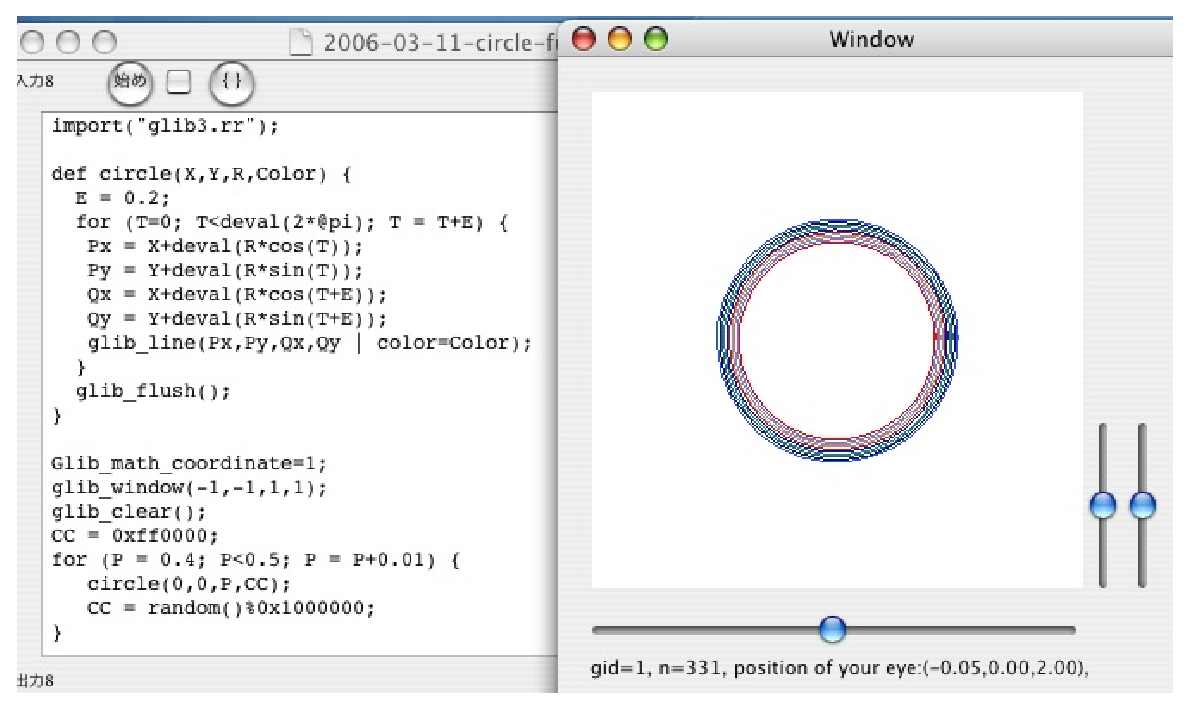
\includegraphics{Figs/circleFunc.eps}}
\caption{ $B4X?t$K$h$kF1?41_$NIA2h(B} \label{fig:circleFunc}
\end{figure}
%>C

$B$5$F1_$rIA$/Nc$K$b$I$m$&(B.
$B0J2<$N$h$&$K4X?t(B {\tt circle(X,Y,R,Color)}$B$rDj5A(B ({\tt def}) $B$9$k(B.
$B$3$N4X?t$r(B $R$ $B$d(B $Color$ $B$rJQ2=$5$;$J$,$i8F$V$3$H$K$h$j(B,
$B?^(B\ref{fig:circleFunc} $B$N$h$&$JF1?41_$N?^$rIA$/$3$H$,2DG=$H$J$k(B.
$B4X?t$K$D$$$F$5$i$K>\$7$/$O(B ``asir $B%I%j%k(B'' $B$r;2>H$7$F$[$7$$(B.

\begin{screen}
\begin{verbatim}
import("glib3.rr"); 

def circle(X,Y,R,Color) {
  E = 0.2;  
  for (T=0; T<deval(2*@pi); T = T+E) {
   Px = X+deval(R*cos(T));
   Py = Y+deval(R*sin(T));
   Qx = X+deval(R*cos(T+E));
   Qy = Y+deval(R*sin(T+E));
   glib_line(Px,Py,Qx,Qy | color=Color);
  }
  glib_flush();
}

Glib_math_coordinate=1;
glib_window(-1,-1,1,1);
glib_clear();
CC = 0xff0000;
for (P = 0.4; P<0.5; P = P+0.01) {
   circle(0,0,P,CC);
   CC = random()%0x1000000;
}
\end{verbatim}
\end{screen}
{\tt (Qx,Qy)} $B$H(B {\tt (Px,Py)} $B$O(B
{\tt E} $B$@$1JP3Q$,0[$k(B.
$B1_$rB?LLBN$G6a;w$7$FIA2h$7$F$$$k(B. \\
-----$B%W%m%0%i%`$N>\$7$$2r@b$^$@(B.

\begin{problem} \rm
\begin{enumerate}
\item $B$3$N%W%m%0%i%`$N4X?t$rMQ$$$F@\$9$kH>7B$NF1$81_$rFs$DIA2h$9$k%W%m%0%i%`$r=q$-$J$5$$(B.
\item $B1_$rEI$jDY$94X?t$r:n$l(B.
\item $BJ,EY4o$rIA$/%W%m%0%i%`$r:n$l(B.
\item ($BH/E82]Bj(B) $B$3$NJ,EY4o(B, $B;e(B, $B$*$b$j(B, $B$o$j$P$7(B, $BHD(B, cfep/asir $B$K$h$k%W%m%0%i%`Ey$rMQ$$$F(B,
$BLZ$d%S%k$N9b$5$rB,Dj$9$k5!3#$H%=%U%H%&%(%"%7%9%F%`$r3+H/$;$h(B.
\end{enumerate}
\end{problem}

\begin{problem} \rm
($B$3$l$OH/E82]Bj(B)  \index{OpenGL}  \index{3$B$8$2$s$0$i$U$#$C$/$9(B@3$B<!85%0%i%U%#%C%/%9(B}
cfep $B$K$O(B OpenGL $B%$%s%?%W%j%?!<$,AH$_9~$s$G$"$k(B.
OpenGL $B$O(B3$B<!85%0%i%U%#%C%/%9$rMQ$$$k%=%U%H%&%(%":n@.$N$?$a$K(B
$BMQ$$$i$l$kLs(B 150$B<oN`$N%3%^%s%I$+$i9=@.$5$l$F$$$k%Q%C%1!<%8$G(B
3$B<!85%0%i%U%#%C%/%9$NI8=`5,3J$N$R$H$D$G$b$"$k(B.
cfep 1.1$B$G$O$=$NCf$N(B 10 $B<e$N%3%^%s%I$rMxMQ$G$-$k(B.

$B$3$N(B OpenGL $B%$%s%?%W%j%?!<$rMQ$$(B,
$BB?LLBN(B(polygon)$B$r:`NA$K$7(B,
cfep$B>e5iJT(B, OpenGL $B$N%W%m%0%i%`$r;29M$K(B
``$B2H(B'' $B$r=q$$$F$_$h$&(B. 
\end{problem}


\noindent
\fbox{\bf $B<B=,$NMn$H$77j(B}\\
\begin{enumerate}
\item unix $BHG(B, windows $BHG$G$O(B asir $B%I%j%k$K$"$k$h$&$K(B
\verb@ end$ @ %$
$B$r%W%m%0%i%`$N:G8e$K=q$+$J$$$H9T$1$J$$$,(B, cfep/asir $B$G$O$3$NL?Na$O(B
$B7W;;%(%s%8%s$NDd;_L?Na$H$J$k$N$G=q$$$F$O$$$1$J$$(B.
$B$?$@$7(B\underline{$B9T$NF,(B}$B$K(B\underline{$B6uGr$r$$$l$:$K(B}$B=q$$$F$"$k(B 
\verb@ end$ @ %$
$B$O<+F0:o=|$5$l$k$N$G(B, unix, windows $BHG6&DL$N%W%m%0%i%`$r=q$/$H$-$O(B
$B6uGr$rF~$l$:$K9T$NF,$K=q$$$F$*$/$HJXMx$G$"$k(B.
\item $B6uGr$d2~9T$O86B'<+M3$KA^F~$7$F$$$$$,(B, $B6uGr$rF~$l$F$O$$$1$J$$I=8=$,$"$k(B.
$B$?$H$($P(B
\begin{verbatim}
0.1
\end{verbatim}
$B$H=q$/$Y$-$H$3$m$r(B
\begin{verbatim}
0. 1
\end{verbatim}
$B$H(B $1$ $B$NA0$K6uGr$rF~$l$k$H%(%i!<$H$J$k(B. 
$B?t;z$K$O6uGr$rF~$l$F$O$$$1$J$$(B.
$BM}M3$O(B asir $B%I%j%k$N9=J82r@O$N>O$rFI$`$HM}2r$G$-$k$H;W$&(B.
\item {\tt sin\ x} $B$J$kI=8=$O<u$1IU$1$F$/$l$J$$(B. 
$BI,$:3g8L$,$$$k(B. $B$D$^$j(B {\tt sin(x)} $B$H=q$/(B.
\item $B3]$1;;$N(B {\tt *} $B$O>JN,$G$-$J$$(B.
\end{enumerate}

\noindent
\HHH.
{\tt [1,2,3]} $B$N$h$&$K(B {\tt []} $B$G0O$C$?I=8=$r%j%9%H(B(list)$B$H8F$V(B.
$B4X?t$NLa$jCM$r?t$NAH$K$7$?$$$H$-$O%j%9%H$rCM$H$7$FLa$9$HNI$$(B.
{\tt print} $BJ8$GB?$/$N?t$r0l9T$GI=<($7$?$$$H$-$b%j%9%H$r;H$&$HJXMx$G$"$k(B.
{\tt L} $B$r%j%9%H$H$9$k$H$-(B {\tt L[0]} $B$G%j%9%H$N:G=i(B(0$BHVL\(B)$B$N85(B,
{\tt L[1]} $B$G%j%9%H$N(B1$BHVL\$N85(B, ... $B$rI=$9(B. 
$B>\$7$/$O(B asir $B%I%j%k;2>H(B.
\begin{screen}
\begin{verbatim}
L=[3,2,1];
print(L);
print(L[0]+L[1]+L[2]);
\end{verbatim}
\end{screen}
%%Note: misc-2010/10/keisan-1/note-ja.txt  $B9V5A$N?JEY(B.

\chapter{For $BJ8$K$h$k?tNs$N7W;;(B}

\section{$BD6F~Lg(B, $BBh(B2$B$N4XLg(B: $BA22=<0$G$-$^$k?tNs$N7W;;(B}

\begin{example} \rm
$a$ $B$r@5$N?t$H$9$k$H$-(B,
\begin{eqnarray*}
  x_{n+1} &=& \frac{x_n + \frac{a}{x_n}}{2}, \\
  x_0 &=& a
\end{eqnarray*}
$B$G$-$^$k?tNs(B $x_0, x_1, x_2, \ldots $ 
$B$O(B $\sqrt{a}$ $B$K$I$s$I$s6aIU$/$3$H(B($B<}B+$9$k$3$H(B)$B$,CN$i$l$F$$$k(B.
$a=2$ $B$N;~(B, $x_1, x_2, \ldots, x_4, x_5$ $B$r7W;;$9$k%W%m%0%i%`$r=q$$$F$_$h$&(B.
%%Prog: cfep/tests/2006-03-11-sqrt.rr
\begin{screen}
\begin{verbatim}
A = 2.0;
X = A;
for (I=0; I<5; I++) {
  Y = (X+A/X)/2; 
  print(Y);
  X = Y;
}
\end{verbatim}
\end{screen}
\end{example}

$B$3$N%W%m%0%i%`$N<B9T7k2L$O?^(B\ref{fig:sqrt}.
%<C
\begin{figure}[tbh]
\scalebox{0.5}{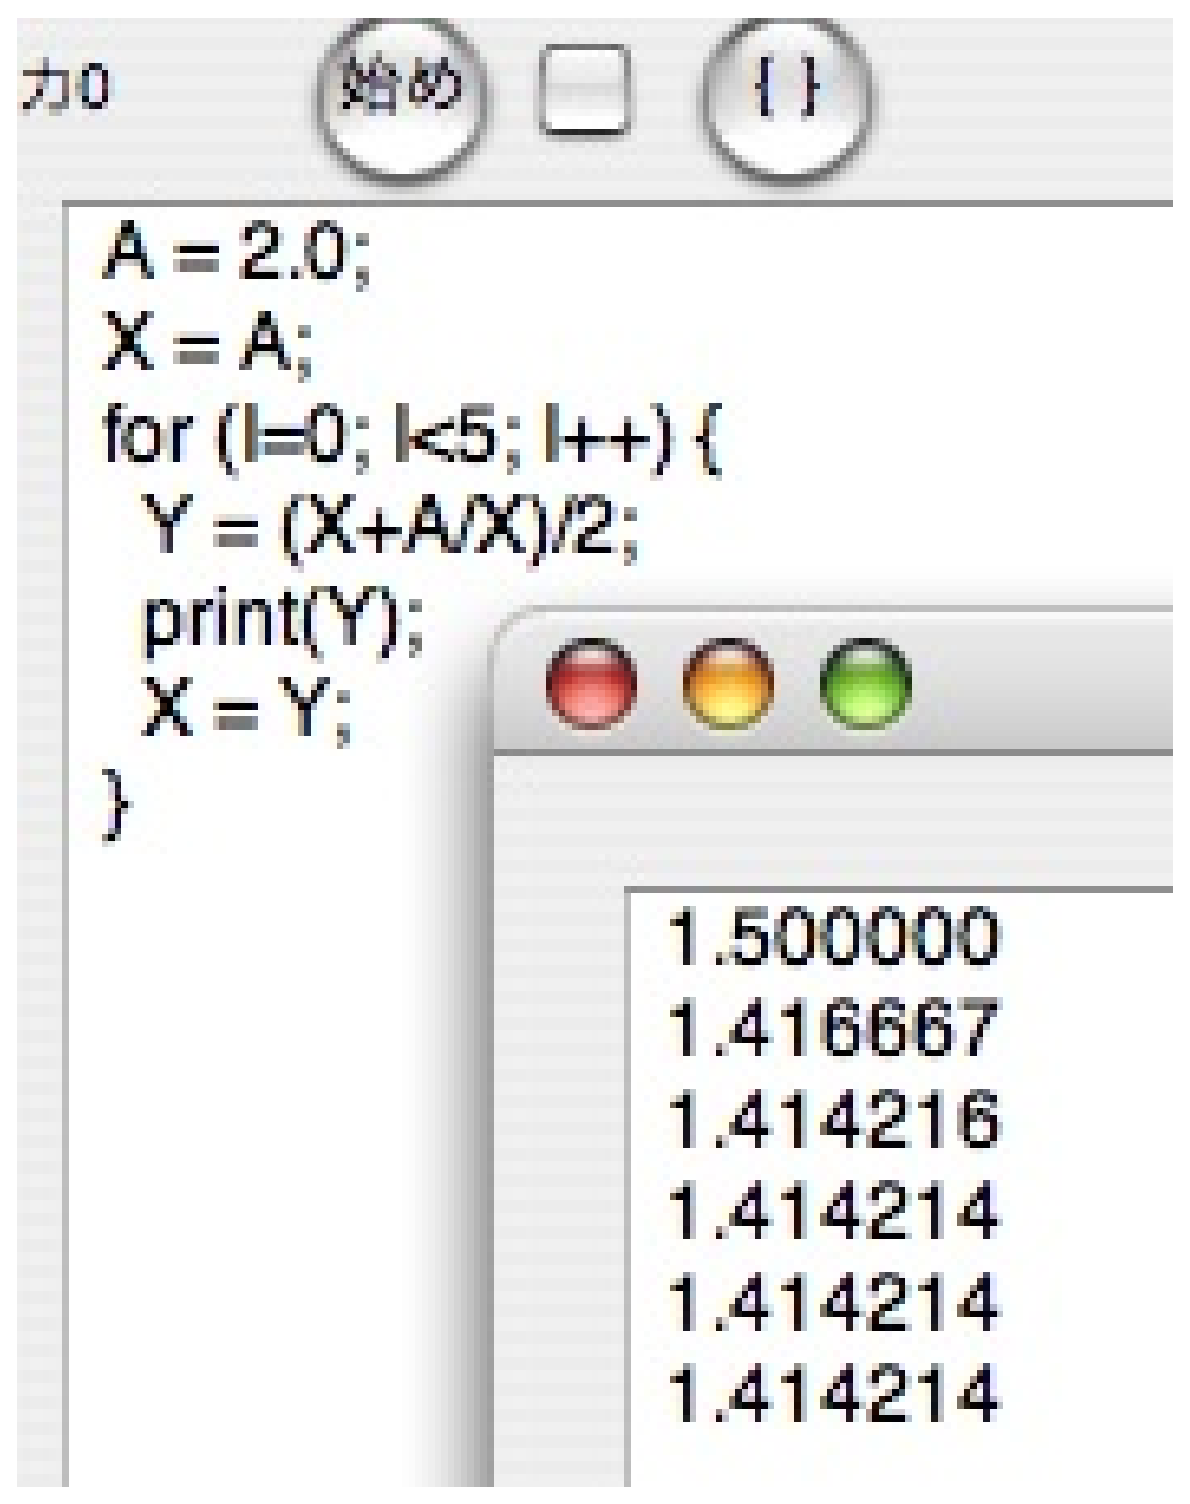
\includegraphics{Figs/sqrt.eps}}
\caption{$\sqrt{2}$ $B$K<}B+$9$k?tNs(B} \label{fig:sqrt}
\end{figure}
%>C

$BD6F~Lg$G$N4XLg$O(B
\begin{screen}
\begin{verbatim}
  Y = (X+A/X)/2; 
  X = Y;
\end{verbatim}
$B$N0UL#$r40A4$KM}2r$9$k$3$H(B
\end{screen}
$B$G$"$k(B.
$BJQ?t$N>O$G@bL@$7$?$h$&$K(B, 
$$  \mbox{{\bf $BJQ?tL>(B}} {\tt = }  \mbox{{\bf $B<0(B}} {\tt  ;} $$
$B$O$^$:1&JU$N<0$r7W;;$7$=$N$"$H$=$N7W;;7k2L$r:8JU$NJQ?t$KBeF~$;$h$H$$$&0UL#(B
$B$G$"$k(B. $B$7$?$,$C$F(B,
\verb@  Y = (X+A/X)/2;  @ $B$O8=:_$N(B {\tt X} $B$H(B {\tt A} $B$K3JG<$5$l$?(B
$B?t;z$r$b$H$K(B \verb@ (X+A/X)/2 @ $B$NCM$r7W;;$7(B, $B$=$N7k2L$rJQ?t(B {\tt Y} $B$XBeF~$;$h(B,
$B$H$$$&0UL#$G$"$k(B. $B$^$?(B
\begin{screen}
\verb@X=Y@ $B$O(B \verb@X@ $B$,(B \verb@Y@ $B$KEy$7$$$H$$$&0UL#$G$O$J$/(B,
$BJQ?t(B\verb@Y@ $B$K3JG<$5$l$??t;z$r(B $BJQ?t(B \verb@X@ $B$KBeF~$;$h$H$$$&0UL#$G$"$k(B.
\end{screen}
$B$3$N$h$&$K9M$($l$P(B, $B>e$N%W%m%0%i%`$,(B $x_1, x_2, x_3, x_4$ $B$NCM$r(B
$B=gHV$K7W;;$7$F(B print $B$7$F$$$kM}M3$,M}2r$G$-$k$G$"$m$&(B.
$B<+J,$,7W;;5!$K$J$C$?$D$b$j$G(B,
$BJQ?t$NCf$N?tCM$,$I$N$h$&$KJQ2=$7$F$$$/$N$+(B,
$B=q$-$J$,$iM}2r$7$FD:$-$?$$(B.
$B$3$l$,$O$C$-$jM}2r$G$-(B, $B1~MQLdBj$,<+M3$K2r$1$k$h$&$K$J$C$?(B, $BD6F~LgB46H$G$"$k(B.
\index{$B$@$$$K$e$&(B@$BBeF~(B}

\begin{problem} \rm
$BJQ?t(B {\tt I}, {\tt X}, {\tt Y} $B$NCM$O(B {\tt for} $B%k!<%WFb$G$I$N$h$&$K(B
$BJQ2=$9$k$+(B?
{\tt Y= (X+A/X)/2} $B$N9T$,<B9T$5$l$kA0$N$3$l$i$NJQ?t$NCM$rI=$K$7$F(B
$B$^$H$a$h(B.  {\tt print([I,X,Y])} $B$r$O$5$`$3$H$K$h$j$3$NI=$,@5$7$$$3$H$r(B
$B$?$7$+$a$h(B.
\end{problem}
$BI=$O<!$N$h$&$J7A<0$G=q$/(B.
\begin{tabular}{|c|c|c|c|c|c|}
\hline
{\tt I} & 0&1&2&3&4 \\ \hline
{\tt X} & &&&& \\ \hline
{\tt Y} & &&&& \\ \hline
\end{tabular}

\begin{problem} \rm
$B%W%m%0%i%`$N%P%0(B(bug)$B$H$O$J$K$+(B? 
\end{problem}

\section{$B1_$rIA$/?tNs(B}

$BA0$N>O$G1_$rIA$/4X?t$r>R2p$7$?(B.
$\sin$,$\cos$ $B$N7W;;$K;~4V$,$+$+$k7W;;5!$G$O(B, $B$J$k$Y$/(B
$B$3$l$i;03Q4X?t$rMQ$$$J$$$G1_$rIA2h$9$kI,MW$,$"$k(B.

$B0l$D$NJ}K!$O(B $s=\tan \frac{t}{2}$ $B$H$*$/$H(B
$\cos t = \frac{1+s^2}{1-s^2}$,
$\sin t = \frac{2s}{1-s^2}$
$B$H=q$1$k$H$$$&8x<0$r;H$&J}K!$G$"$k(B.
$s$ $B$O%?%s%8%'%s%H$GDj5A$5$l$F$$$k$3$H$rK:$l$F$7$^$($P$h$$(B.  

$B$b$&0l$D$O(B
$B?tNs$N7W;;$rMQ$$$F(B, $\cos$ $B$d(B $\sin$ $B$N7W;;$r$d$i$:$K1_$rIA$/(B
$BJ}K!$G$"$k(B.
%%Prog: cfep/tests/2006-03-11-circle-dda.rr
\begin{screen}
\begin{verbatim}
import("glib3.rr");
Glib_math_coordinate=1;
glib_window(-2,-2, 2,2);
glib_clear();
E = 0.1;   
C1 = 1.0; C2=1.0;
S1 = 0.0; S2=E; 
for (T=0; T<=deval(2*@pi); T = T+E) {
    C3 = 2*C2-C1-E*E*C2;
    S3 = 2*S2-S1-E*E*S2;
    glib_line(C1,S1, C2,S2); 
    C1=C2; S1=S2;
    C2=C3; S2=S3;
    glib_flush(); 
}
\end{verbatim}
\end{screen}

$B$3$N%W%m%0%i%`$N<B9T7k2L$O?^(B\ref{fig:circleDda}.
%<C
\begin{figure}[tbh]
\scalebox{0.6}{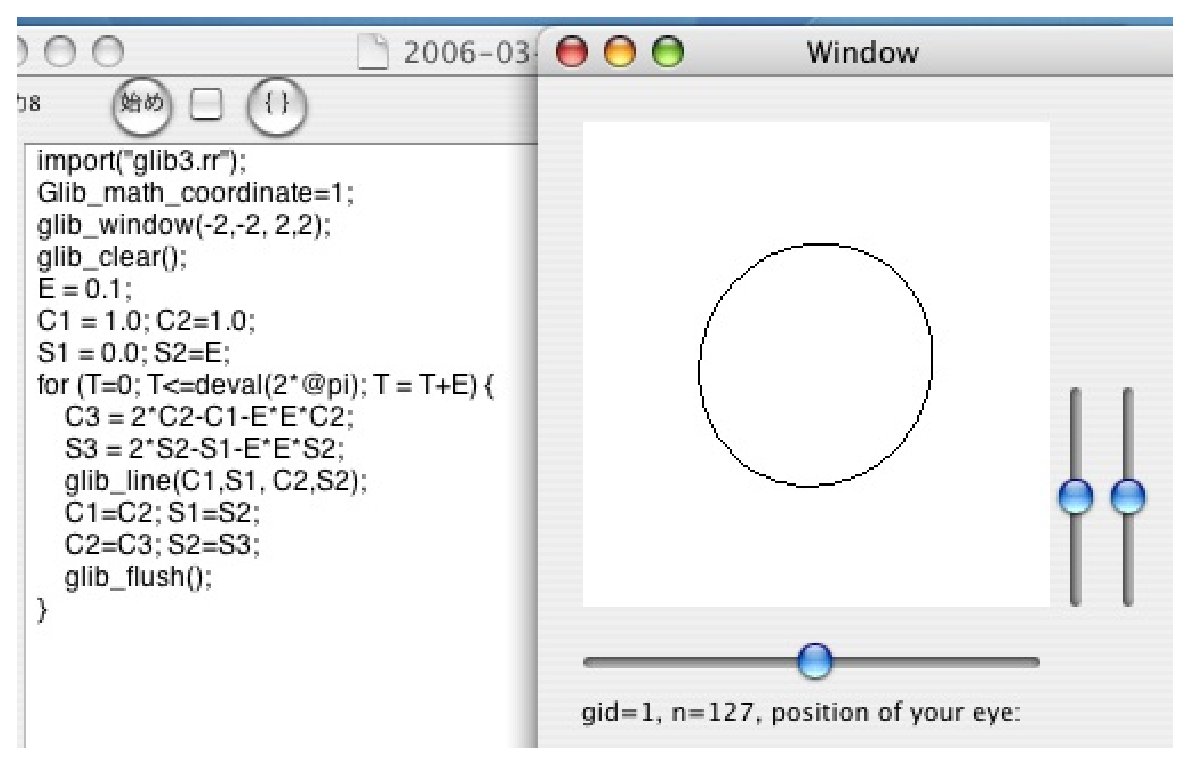
\includegraphics{Figs/circleDda.eps}}
\caption{$\cos$, $\sin$ $B$r;H$o$:$K1_$rIA$/(B} \label{fig:circleDda}
\end{figure}
%>C

-----$B%W%m%0%i%`$N2r@b$^$@=q$$$F$J$$(B.

$B%R%s%H(B: 
$BHyJ,J}Dx<0(B $d^2 x/dt^2 = -x, d^2 y/dt^2 = -y$ $B$r(B $t$ $B$r%i%8%"%s$H$7$F(B
$B:9J,K!$G6a;wE*$K2r$$$F$$$k(B.

$B$3$NOCBj$O(B, $B?tNs$N7W;;$H:9J,J}Dx<0$K$h$k%7%_%e%l!<%7%g%s$KB3$/(B.
$B$3$l$K$D$$$F$O$^$?9F$r$"$i$?$a$F=q$$$F$_$?$$(B.

$B0J>e$GD6F~Lg$O=*N;$G$"$k(B.  $BB3$-$O(B ``Asir $B%I%j%k(B'' $B$rFI$s$G$M(B. 
$BFC$KG[Ns$H4X?t$r%^%9%?!<$9$k$H?t3X%W%m%0%i%`$K$O=EJu$9$k(B.

$B$J$*(B, asir $B%I%j%k$K>R2p$7$F$"$k%W%m%0%i%`$O(B \verb@ end$ @  %$
$B$^$?$O(B \verb@ end; @ $B$,:G8e$K=q$$$F$"$k>l9g$,B?$$$,(B,
cfep/asir $B$G$O$3$N(B {\tt end} $B$r=q$$$F$O$$$1$J$$(B.
{\tt end } $B$O7W;;%(%s%8%s$NDd;_L?Na$G$"$j(B, $B<B9T$5$l$k$H(B ``$B7W;;Cf$NI=<((B'' $B$,$G$FL51~Ez$H$J$k(B.
($B0l1~(B, $B9TF,$K$"$k$3$l$i$NL?Na$O<+F0E*$K:o=|$9$k$h$&$K$J$C$F$O$$$k(B.)
%% kxx/ox_texmacs.c

\begin{problem} \rm
($B%l%]!<%HLdBj$NNc(B) \\
$B$J$K$+?^$rIA$/%W%m%0%i%`$r=q$-$J$5$$(B. ($BDjHV%I%i%(%b%s$G$b$h$$(B)
\end{problem}

\noindent
\fbox{$B%N!<%H(B}.
$BCx<T$N>l9g(B, $B=5$K(B1$B%3%^9V5A(B, $B1i=,(B1$B%3%^$G$O(B, $B$3$3$^$G$G(B3$B=5$G$"$k(B.
$B>e$N%l%]!<%HLdBj$,:G=i$N%l%]!<%H(B.
3$B=5L\$N1i=,$N;~4V$+$i$H$j$+$+$j(B, 5$B=5L\$N1i=,$N;~4V$KH/I=(B.
4$B=5L\$+$i$O(B asir$B%I%j%k(B.

\chapter{cfep $B>e5iJT(B}

\section{\TeX $B$K$h$k%?%$%W%;%C%H(B($B<B83E*(B)}
%%Doc: cfep/tests/2006-03-06
$B=PNO$r(BTeX$B$G%?%$%W%;%C%H$9$k$K$O(B 
``$B<B9T(B'' $B%a%K%e!<$+$i(B ``$B=PNO$r(BTeX$B$G%?%$%W%;%C%H(B'' $B$rA*Br$9$k(B.
{\tt latex}, {\tt dvipng} $B$,%$%s%9%H!<%k$5$l$F$$(B
$B$J$$$HF0:n$7$J$$(B.
$B$3$l$i$O$?$H$($P(B {\tt fink}  $B$+$i(B \TeX $B$r%$%s%9%H!<%k$7$?$j(B,
{\tt ptex\_package\_2005v2.1.dmg} ($B:G6a$N>u67$O(B ptex package macosx $B$G8!:w(B)
$B$J$I$G(B Mac $BMQ$N(B pTeX $B$r%$%s%9%H!<%k$7$F$*$1$P$h$$(B.
\TeX $B$rMQ$$$?;E>e$jNc$O?^(B\ref{fig:sl2}$B$r8+$h(B. 
$B$J$*(B, \TeX $B$G%?%$%W%;%C%H$9$k>l9g%[!<%`$N2<$K(B
\verb@OpenXM_tmp@ $B$J$k:n6HMQ$N%U%)%k%@$,:n@.$5$l$k(B.
$B%?%$%W%;%C%H$O<B835!G=$N$?$a(B, $B$3$N%U%)%k%@$NCf$N:n6HMQ%U%!%$%k$O<+F0$G$O>C5n$5$l$J$$(B.
$B;~!9<jF0$G:n6H%U%!%$%k$r>C5n$5$l$?$$(B.
\index{tex@\TeX}

\section{$BA*BrHO0O$N$_$N<B9T(B}

\index{$B$;$s$?$/$O$s$$$N$_$N$8$C$3$&(B@$BA*BrHO0O$N$_$N<B9T(B}
$B2hLL>e$N(B ``$BA*BrHO0O$N$_$r<B9T(B'' $B$r%A%'%C%/$9$k$H(B,
``$B;O$a(B'' $B%\%?%s$r$*$7$?$H$-(B, $BA*BrHO0O$N$_$,I>2A$5$l$k(B.
$BA*BrHO0O$,$J$$>l9g$O%-%c%l%C%H0LCV$N9T$,<+F0A*Br$5$l$F<B9T$5$l$k(B.
\command{{\tt Enter}} $B$HAH$_9g$o$;$F$3$N5!G=$r;H$&$H(B, $B%?!<%_%J%k$+$i(B 
asir $B$rMxMQ$9$k$N$K$A$g$C$H;w$F$/$k(B.
$B?^(B\ref{fig:sl2}$B$O$3$N$h$&$J<B9T$r$7$F$$$kNc$G$"$k(B.

%<C
\begin{figure}[tbh]
\scalebox{0.5}{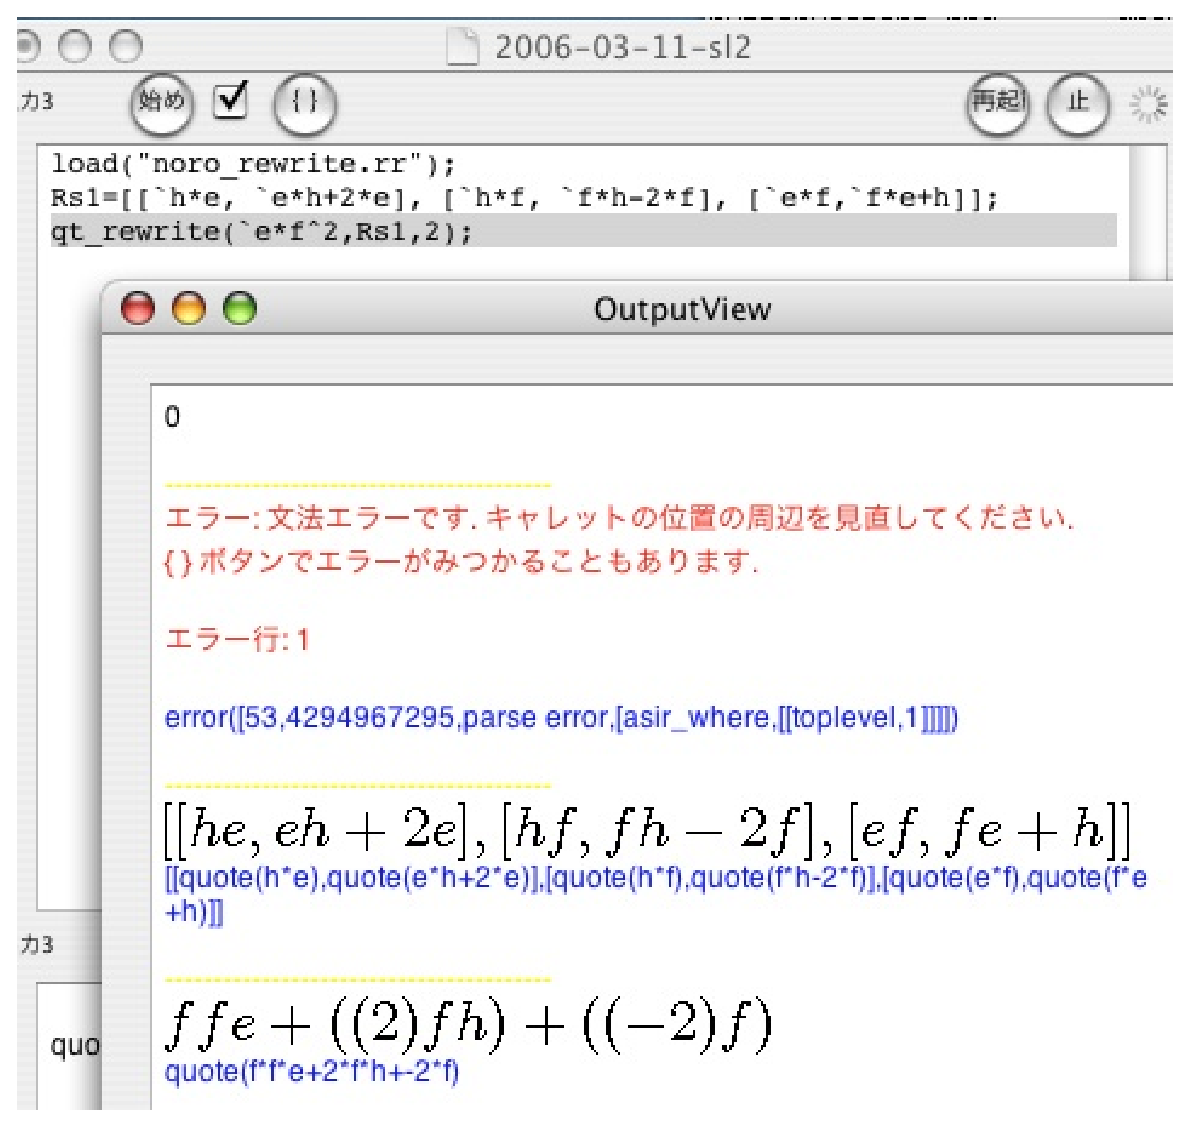
\includegraphics{Figs/sl2.eps}}
\caption{$B%?!<%_%J%kIw(B} \label{fig:sl2}
\end{figure}
%>C


\noindent
%%Doc:  cfep/tests/2007-03-07-debug.rtfd
\fbox{$B<ALd(B}
cfep $B$N%$%s%?%U%'!<%9$G%G%P%C%0$r$7$J$,$i%W%m%0%i%`$r3+H/$9$k$K$O$I$N$h$&$K$d$k$H(B
$B$h$$$+(B? \\
\fbox{$BEz$((B}
cfep $B$O=i?4<T8~$-$N%$%s%?%U%'!<%9$J$N$G(B,
$BBg5,LO$J%W%m%0%i%`3+H/$rA[Dj$7$F$$$J$$$,(B, 
$B;d$O<!$N$h$&$K%i%$%V%i%j$N3+H/$r$7$F$$$k(B.

\begin{enumerate}
\item $BI,MW$J4X?t$r=q$/(B. $B2<$NNc$G$O(B {\tt sum1}.
\item $B4X?t$r%F%9%H$9$kF~NO$r%3%a%s%H$N7A$G$=$N4X?t$N6a$/$K=q$$$F$*$/(B.
$B2<$NNc$G$O%3%a%s%H$K$"$k(B {\tt sum1(10,1); } $BEy(B.
\end{enumerate}


\begin{screen}
\begin{verbatim}
/*
testinput:  sum1(10,1);
testinput:  sum1(10,2);
*/
def sum1(N,M) {
  S = 0; i=1;
  for (I=1; I<N; I++) {S = S+I^M; }
  return S;
}
\end{verbatim}
\end{screen}

\begin{enumerate}
\item ``$B;O$a(B'' $B%\%?%s$G4X?tDj5A$r%m!<%I(B. 
$B$3$N;~E@$GJ8K!%(%i!<$J$I$,$"$l$P%a%C%;!<%8$K$7$?$,$C$F=$@5(B.
\item $B$=$N$"$H(B ``$BA*BrHO0O$N$_$r<B9T(B'' $B$N%b!<%I$KJQ99$7$F%3%a%s%HFb$N(B testinput $B$r<B9T(B.
\item $B<B9T;~$N%(%i!<$N9THV9f$X$N0\F0$O(B "$BA*BrHO0O$N$_$r<B9T(B" $B$N%b!<%I$r2r=|$7$F$+$i(B
$B9T$&(B.   \index{$B$($i!<(B@$B%(%i!<(B}
\end{enumerate}

%<C
\begin{figure}[tb]
\scalebox{0.5}{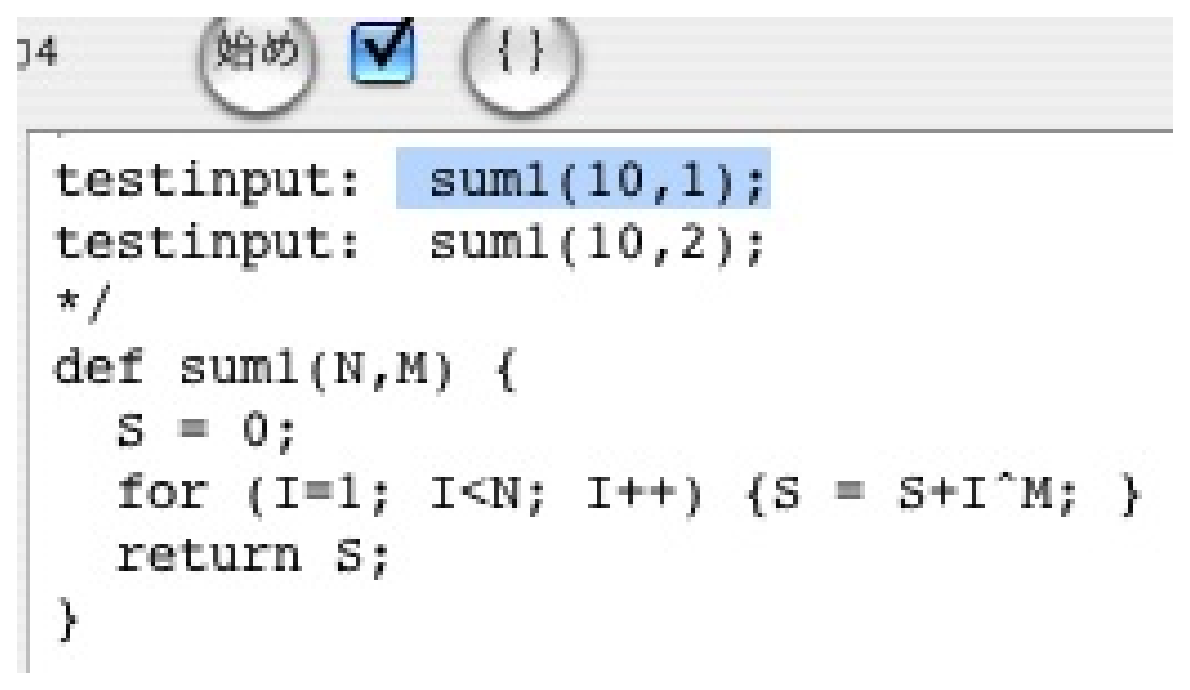
\includegraphics{Figs/howtoDebug1.eps}}
\caption{``$BA*BrHO0O$N$_$r<B9T(B''$B$N3hMQ(B} \label{fig:howtoDebug1}
\end{figure}
%>C


\section{$B%(%s%8%s$r5/F0$7$J$$(B}
%%cfep/tests/2006-03-08-noEngine

\noindent
\fbox{$B<ALd(B}
 $B%F%-%9%HJT=8$^$?$O%F%-%9%H$N1\Mw$@$1$G7W;;$r$9$k$D$b$j$O$"$j$^$;$s$,(B. \\
\fbox{$BEz$((B} 
   ``$B<B9T(B'' $B%a%K%e!<$G(B ``$B%(%s%8%s$r<+F05/F0$7$J$$(B'' $B$rA*Br(B. \\
%<C
\scalebox{0.3}{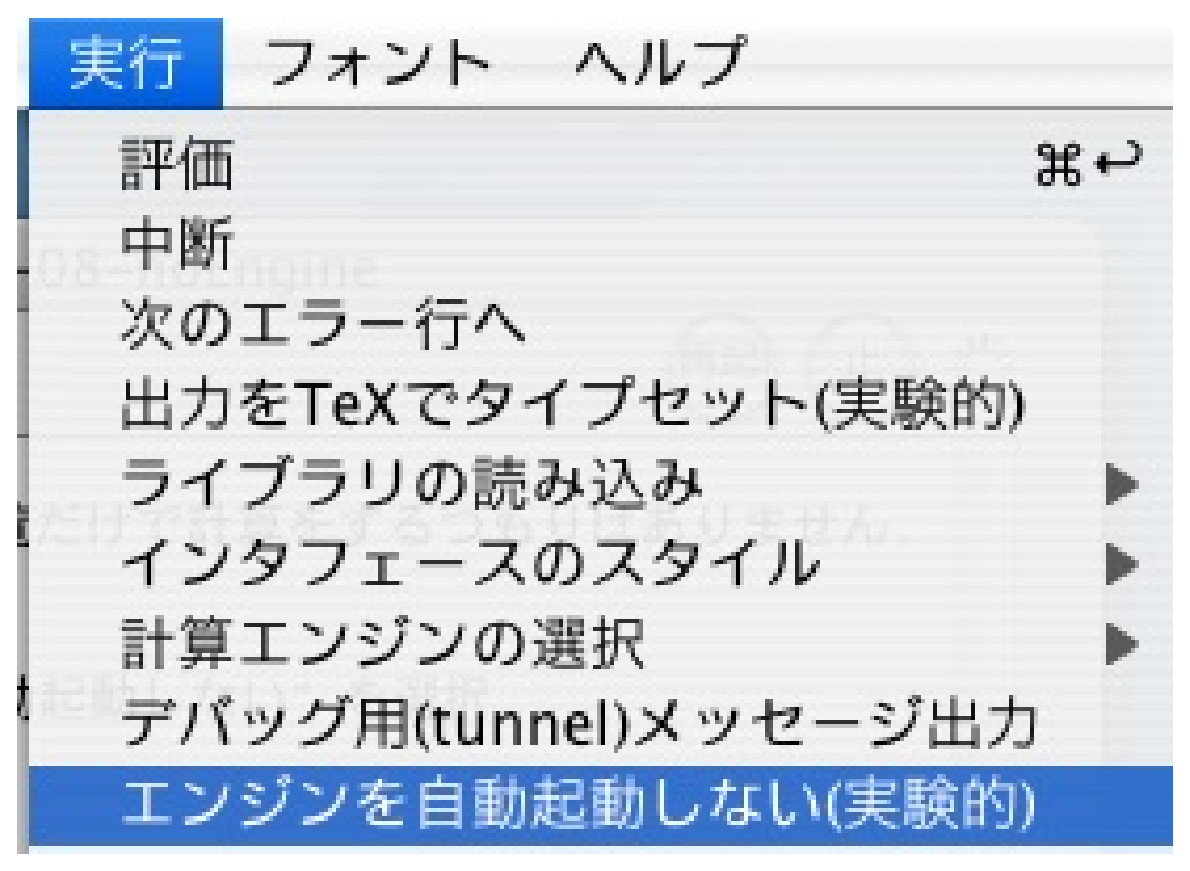
\includegraphics{Figs/menuNoEngine.eps}} \\
%>C
$B$"$H$G%(%s%8%s$r5/F0$7$?$$>l9g$O(B  ``$B:F5/(B'' $B%\%?%s$r$*$7$F%(%s%8%s$r5/F0$9$k(B. \\
%<C
\scalebox{0.3}{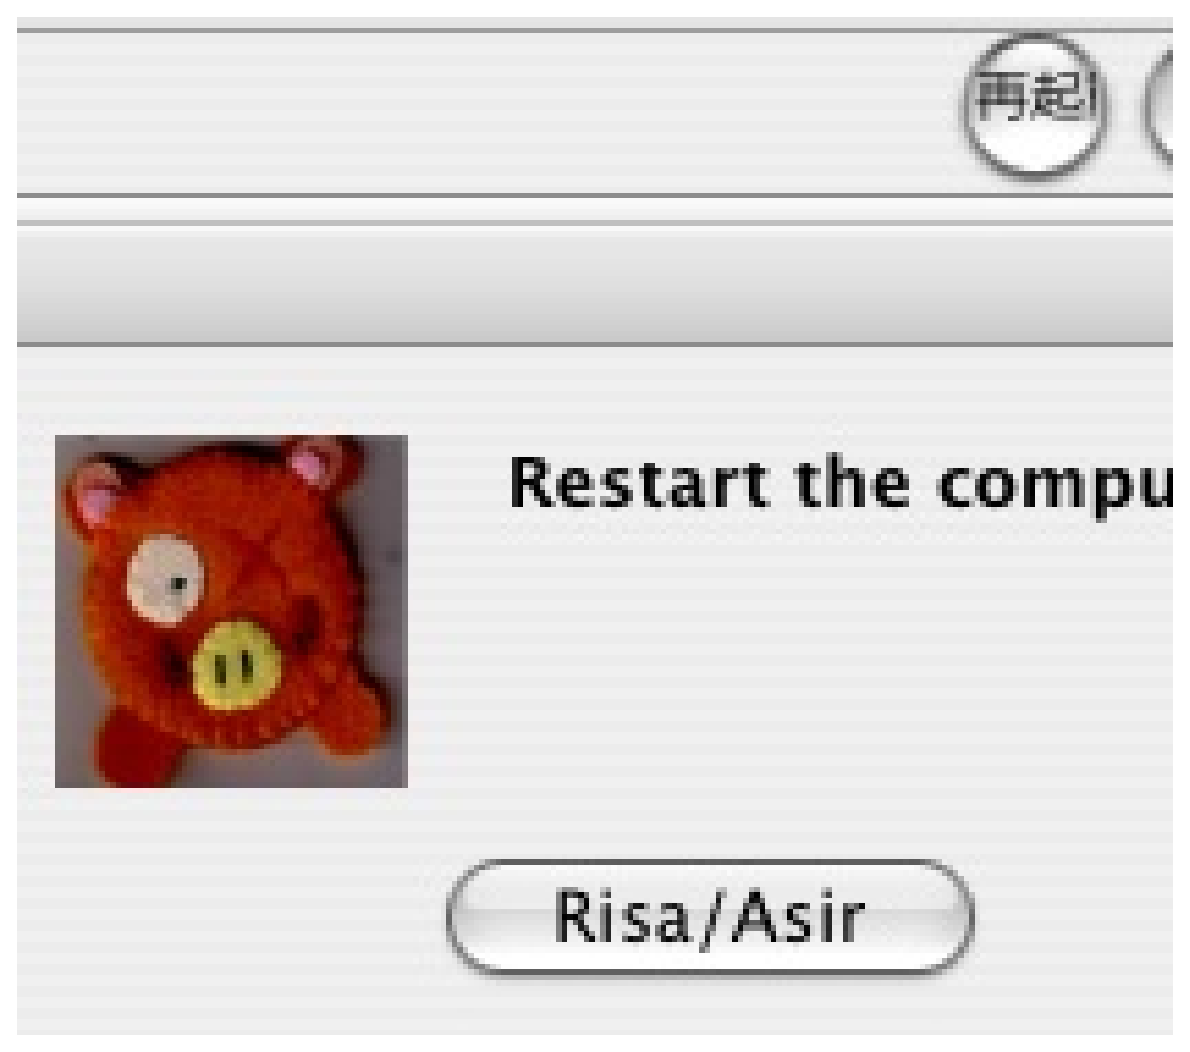
\includegraphics{Figs/popupRestart.eps}}
%>C


\section{OpenGL$B%$%s%?%W%j%?(B}

\index{OpenGL}
Cfep $B$K$O(B OpenGL $B%$%s%?%W%j%?!<$,AH$_9~$s$G$"$k(B.
OpenGL $B$O(B3$B<!85%0%i%U%#%C%/%9$rMQ$$$k%=%U%H%&%(%":n@.$N$?$a$K(B
$BMQ$$$i$l$kLs(B 150$B<oN`$N%3%^%s%I$+$i9=@.$5$l$F$$$k%Q%C%1!<%8$G(B
3$B<!85%0%i%U%#%C%/%9$NI8=`5,3J$N$R$H$D$G$b$"$k(B.
cfep 1.1$B$G$O$=$NCf$N(B 10 $B<e$N%3%^%s%I$rMxMQ$G$-$k(B.
$B>\$7$/$O(B
{\tt cfep.app/OpenXM/lib/asir-contrib/cfep-opengl.rr} $B$r;2>H(B.

\index{OpenGL$B$0$i$U$#$C$/$*$V$8$'$/$H(B@OpenGL$B%0%i%U%#%C%/%*%V%8%'%/%H(B}
OpenGL $B$G$O$^$:(B OpenGL$B%0%i%U%#%C%/%*%V%8%'%/%H$rG[CV$7(B,
$B$=$l$+$i;kE@$N0LCV$+$i8+$?2hA|$rIA2h$9$kJ}K!$rMQ$$$k(B.
$B$7$?$,$C$F(B, $B%7%9%F%`$O>o$K(B OpenGL$B%0%i%U%#%C%/%*%V%8%'%/%H$N=89g$rJ];}(B
$B$7$F$$$k(B.
{\tt glib\_remove\_last()} $BL?Na$O$=$N:G8e$NMWAG$r:o=|$9$kL?Na$G$"$k(B.
{\tt cfep-opengl.rr} $B%i%$%V%i%j$G$O(B,
{\tt opengl.metaRemoveLast()} $B4X?t$G:G8e$NMWAG$r:o=|$G$-$k(B.
\index{opengl}

%<C
\begin{figure}[tb]
\scalebox{0.6}{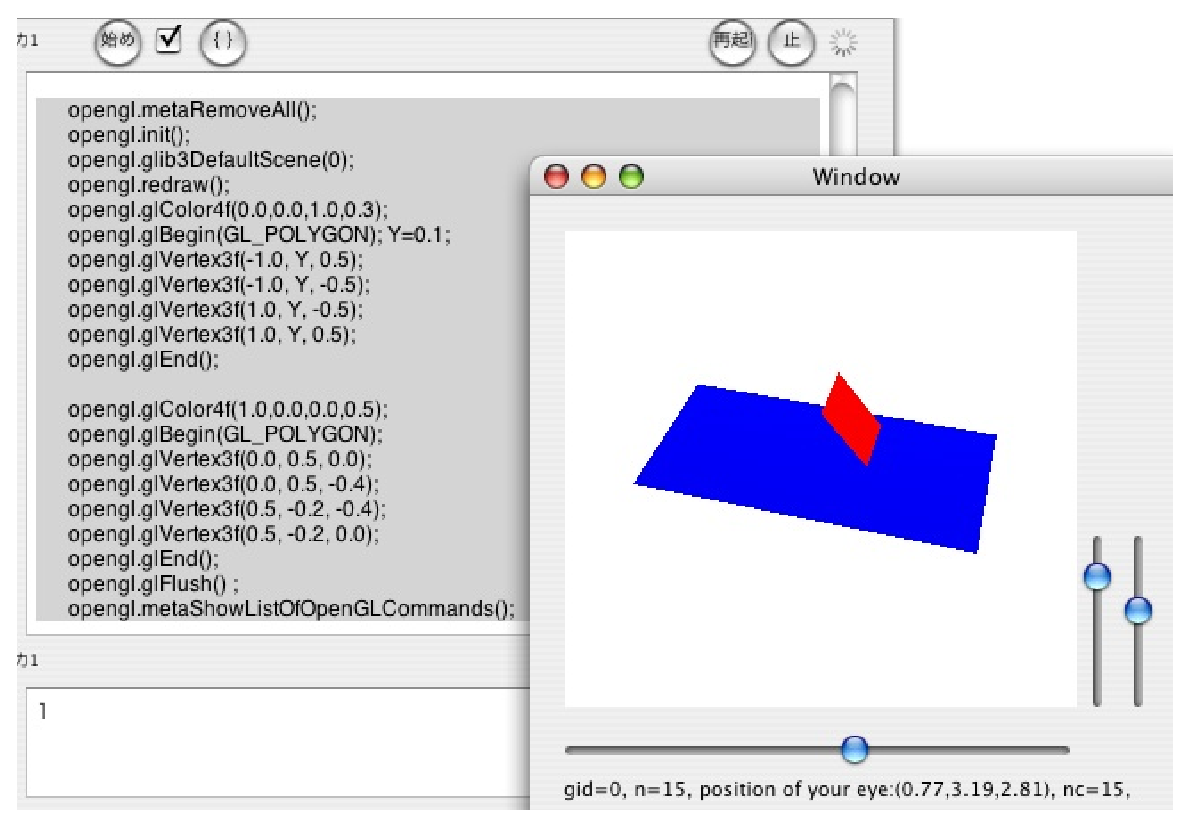
\includegraphics{Figs/twoPolygon.eps}}
\caption{} \label{fig:twoPolygon}
\end{figure}
%>C

\begin{screen}
\begin{verbatim}
      import("cfep-opengl.rr");
      opengl.metaRemoveAll();
      opengl.init();      
      opengl.glib3DefaultScene(0);
      opengl.redraw(); 
      opengl.glColor4f(0.0,0.0,1.0,0.3);  
      opengl.glBegin(GL_POLYGON); Y=0.1;
      opengl.glVertex3f(-1.0, Y, 0.5);
      opengl.glVertex3f(-1.0, Y, -0.5);
      opengl.glVertex3f(1.0, Y, -0.5);
      opengl.glVertex3f(1.0, Y, 0.5);
      opengl.glEnd();

      opengl.glColor4f(1.0,0.0,0.0,0.5); 
      opengl.glBegin(GL_POLYGON);
      opengl.glVertex3f(0.0, 0.5, 0.0);
      opengl.glVertex3f(0.0, 0.5, -0.4);
      opengl.glVertex3f(0.5, -0.2, -0.4);
      opengl.glVertex3f(0.5, -0.2, 0.0);
      opengl.glEnd();
      opengl.glFlush() ; 
      opengl.metaShowListOfOpenGLCommands();
\end{verbatim}
\end{screen}
$B$3$N%W%m%0%i%`$G$O(B 2 $BKg$ND9J}7A$rIA$$$F$$$k(B.
$B$3$N%W%m%0%i%`$N=PNO$O?^(B\ref{fig:twoPolygon}.
-----$B>\$7$$@bL@$O$^$@(B.

OpenGL $B$N2hLL$K$OIaDL$N?t3X$N$h$&$K(B $(x,y)$ $B:BI8$,$O$$$C$F$*$j(B,
$B2hLL$+$i<jA0B&$,(B $z$ $B:BI8$,@5$NJ}8~(B, $B2hLL$N8~$3$&B&$,(B
$z$ $B:BI8$,Ii$NJ}8~$G$"$k(B. 
``$BL\(B'' $B$+$i86E@J}8~$r8+$?2hA|$,(B
$B?^(B\ref{fig:twoPolygon}$B$K$"$k$h$&$K(B 3 $B$D$N%9%i%$%@!<$rMQ$$$FL\$N0LCV$rF0$+$;$k$N$G(B,
OpenGL$B%*%V%8%'%/%H$r$$$m$$$m$J3QEY$+$i$_$k$3$H$,2DG=$G$"$k(B.
$B2<$N%9%i%$%@!<$,L\$N(B $x$ $B:BI8(B, $B1&$NFs$D$N%9%i%$%@!<$,$=$l$>$lL\$N(B $y$, $z$ $B:BI8$G$"$k(B.
$BL\$NF0$-$K47$l$k$K$O(B, $B<!$NFs$D$N%G%b2hLL$r$?$a$9$HLLGr$$$@$m$&(B.
\begin{screen}
\begin{verbatim}
import("cfep-opengl.rr");
opengl.glib3DefaultScene("mesa demo/ray");
\end{verbatim}
\end{screen}

\begin{screen}
\begin{verbatim}
import("cfep-opengl.rr");
opengl.glib3DefaultScene("cfep demo/icosahedron");
\end{verbatim}
\end{screen}

\section{asir $B0J30$N7W;;%(%s%8%s$NMxMQ(B}

cfep$B$+$i(B asir $B0J30$N(B OpenXM $B=`5r$N7W;;%(%s%8%s$bMxMQ$G$-$^$9(B.
$B$?$H$($P(B, $B<B9T(B, $B7W;;%(%s%8%s$NA*Br$G(B, kan/sm1 $B$rMxMQ$9$k$3$H$b2DG=$G$9(B.
cfep, {\tt ox\_texmacs}, {\tt ox\_sm1} $B$,Aj8_$KDL?.$7$J$,$i7W;;$7$F$$$^$9(B.

$B$J$*(B kan/sm1 $B$N(B {\tt run} $B%3%^%s%I$O;H$($^$;$s(B.
\begin{verbatim}
[(parse) ($B%U%!%$%kL>(B)  pushfile] extension 
\end{verbatim}
$B$GBeMQ$7$F2<$5$$(B.

\cleardoublepage
\flushbottom
\printindex

\end{document}